\ifnum\switch=1
% -----------------------------------------------------------------------------
% ------------------------------ Extended ToC ---------------------------------
% -----------------------------------------------------------------------------

Parts of this chapter have already been published in:
\begin{enumerate}
\item[\cite{EchLieNab18}] \underline{C.~Echeverr{\'\i}a}, J.~Liesen, and R.~Nabben, \textbf{Block diagonal dominace of matrices revisited: Bounds for the norms of inverses and eigenvalue inclusion sets}, Linear Algebra Appl., 553 (2018), pp. 365--383.
\end{enumerate}


\section{Introduction}
This section is based on the following references: \cite{BerPle94, FonPet01, Ike79, Nabben99, Nabben99-2, Usm94, Yue06}.
\paragraph{Keywords:} Block Diagonal Dominance, Convergence radius, etc


\section{Bounds on the Inverses of Block Tridiagonal Matrices}
This section is based on the following references: \cite{EchLieNab18}.
\paragraph{Keywords:} Block Tridiagonal Matrices


\section{Inclusion Sets for Eigenvalues}
This section is based on the following references: \cite{Var11}.
\paragraph{Keywords:} eigenvalues, Gershgorin sets.


\section{Numerical Illustrations}
This section is based on the following references: \cite{EchLieNab18}.
\paragraph{Keywords:} convergence, etc.


\else
% -----------------------------------------------------------------------------
% --------------------------- Content of Chapter ------------------------------
% -----------------------------------------------------------------------------

Parts of this chapter have already been published in:
\begin{enumerate}
\item[\cite{EchLieNab18}] \underline{C.~Echeverr{\'\i}a}, J.~Liesen, and R.~Nabben, \textbf{Block diagonal dominace of matrices revisited: Bounds for the norms of inverses and eigenvalue inclusion sets}, Linear Algebra Appl., 553 (2018), pp. 365--383.
\end{enumerate}
%
\vspace{0.25cm}
%
\section{Introduction}
\label{BDiDo:intro}
The main tool that is used for proving the convergence of the multiplicative Schwarz method in Theorems~\ref{thm:1D:upwind_conv} and \ref{thm:1D:central_conv} is Lemma~\ref{lem:1D:MMat}, which characterizes the decay away from the diagonal shown by the entries of the inverse of a tridiagonal Toeplitz matrix whenever it possesses the property of diagonal dominance and its sub- and super-diagonal entries have opposite signs. With the objective of deriving an equally powerful tool that can be applied to the matrices that arise in the discretization of higher dimensional convection-diffusion problems (treated in the Chapter~\ref{ch:2D}), we now present a generalization of the classical theory of diagonal dominance of matrices from the scalar to the block case.

Matrices that are characterized by off-diagonal decay, or more generally
``localization'' of their {entries}, appear in applications throughout the
mathematical and computational sciences. The presence of such localization can
lead to  computational savings, since it allows to approximate a
given matrix by only using its significant entries, and discarding the
negligible ones according to a pre-established criterion. In this context it is
then of great practical interest to know a priori how many and which of these
entries can be discarded as insignificant. Many authors have therefore studied
decay rates for different matrix classes and functions of matrices; see,
\linebreak
e.g.,~\cite{BenBoi14,BenGol99,BenRaz07,BenSim15,CanSimVer14,DemMosSmi84,KriStrWer15,PelPol01}. For an excellent survey of the current state-of-the-art we refer to~\cite{Ben16}.

An important example in this context is given by the (nonsymmetric) diagonally
dominant matrices, and in particular the diagonally dominant tridiagonal
matrices, which were studied, e.g., in~\cite{Nabben99-2,Nabben99}. As shown in
these works, the entries of the inverse decay with an exponential rate along a
row or column, depending on whether the given matrix is row or column
diagonally dominant; see~\cite[\S~3.2]{Ben16} for a more general treatment
of decay bounds for the inverse and further references.

Our main goal in this chapter is to generalize results of~\cite{Nabben99} from
scalar to block tridiagonal matrices. In order to do so, we
use a generalization of the classical definition of block diagonal dominance of
Feingold and Varga~\cite{FeiVar62} to derive bounds and decay rates for the
block norms of the inverse of block tridiagonal matrices of the form
\begin{equation}\label{eq:BDiDo:blocktridiag}
\A=\left[ \begin{array}{crrrr}
\A_1	& 	\B_1 & 					&					 &\\
\C_1	&	\A_2	 & \B_2			&					 &\\
			& \ddots & \ddots 	& \ddots 	 & \\
			&				 & \C_{n-2} & \A_{n-1} & \B_{n-1}\\
			&				 & 					& \C_{n-1} & \A_{n}
\end{array} \right],\quad \mbox{where $\A_i,\B_i,\C_i\in {\mathbb C}^{m\times m}$.}
\end{equation}
We also show how to improve these bounds iteratively (Section~\ref{BDiDo:bounds}).
Moreover, we obtain a new variant of the Gershgorin Circle Theorem for general
block matrices of the form
%
\begin{equation}\label{eq:BDiDo:blockmat}
\A=[\A_{ij}]\quad
\mbox{with blocks $\A_{ij}\in\mathbb{C}^{m\times m}$ for $i,j=1,\dots,n$,}
\end{equation}
which can provide tighter spectral inclusion regions than those
obtained by Feingold and Varga (Section~\ref{BDiDo:Gershgorin}). Throughout
this chapter we assume that $\|\cdot\|$ is a given submultiplicative matrix
norm.

% Although the results presented in this chapter can be applied for analyzing the convergence of the multiplicative Schwarz method, the theory is much more general. The variant of the Gershgorin Circle Theorem applies to  and they apply to any block matrix

\section{Bounds on the Inverses of Block Tridiagonal Matrices}
\label{BDiDo:bounds}

We start with a definition of block diagonally dominant matrices.

\begin{definition}\label{def:BDiDo:bdd}
Consider a matrix of the form \eqref{eq:BDiDo:blockmat}.
%
% \begin{equation}\label{eq:BDiDo:blockmat}
% \A=[\A_{ij}]\quad
% \mbox{with blocks $\A_{ij}\in\mathbb{C}^{m\times m}$ for $i,j=1,\dots,n$.}
% \end{equation}
%
The matrix $\A$ is called \emph{row block diagonally dominant} (with respect to
the matrix norm $\|\cdot\|$) when the diagonal blocks $\A_{ii}$ are nonsingular,
and
%the following conditions hold simultaneously:

\begin{equation}\label{eq:BDiDo:blocdiagdom1}
\sum_{\atopfrac{j=1}{j\neq i}}^{n}\|\A_{ii}^{-1}\A_{ij}\|\leq 1,\quad\text{for $i=1,\dots,n$.}
\end{equation}
%\begin{equation}\label{eq:blocdiagdom2}
%\sum_{\atopfrac{j=1}{j\neq i}}^{n}\|A_{ij}A_{ii}^{-1}\|\leq 1,\quad\text{for $i=1,\dots,n$.}
%\end{equation}
If a strict inequality holds in \eqref{eq:BDiDo:blocdiagdom1}
% and \eqref{eq:blocdiagdom2},
then $\A$ is called \emph{row block strictly diagonally dominant}
(with respect to the matrix norm $\|\cdot\|$).
\end{definition}

Obviously, an analogous definition of \emph{column} block diagonal dominance is
possible. Most of the results in this chapter can be easily rewritten for that
case (see Definition~\ref{def:App:colbdd} in Appendix~\ref{App:BDiDo:ColBDiDo}
and the discussion thereafter). A similar definition recently presented in
\cite{BenEvaHamLupSla17} in an application of block diagonal preconditioning
where the authors call a matrix block diagonally dominant when all its diagonal
blocks are nonsingular, and \eqref{eq:BDiDo:blocdiagdom1} or the analogous
conditions with $\A_{ij}\A_{ii}^{-1}$ replacing $\A_{ii}^{-1}\A_{ij}$ hold
in the $1$-norm, i.e., it does not consider both conditions to hold
simultaneously and it is restricted to the $1$-norm.
%A very similar definition developed by Benzi, et.al., which appears in \cite{BenEvaHamLupSla17}, uses conditions \eqref{eq:BDiDo:blocdiagdom1} and \eqref{eq:blocdiagdom2}

The above definition of row block diagonal dominance generalizes the one of
Feingold and Varga given in \cite[Definition~1]{FeiVar62}, who considered a
matrix as in \eqref{eq:BDiDo:blockmat} block diagonally dominant when the
diagonal blocks $\A_{ii}$ are nonsingular, and
%
\begin{equation}\label{eq:BDiDo:blocdiagdomFV}
\sum_{\atopfrac{j=1}{j\neq i}}^{n}\|\A_{ij}\|\leq(\|\A_{ii}^{-1}\|)^{-1},\quad\text{for $i=1,\dots,n$}.
\end{equation}
%
It is clear that if a matrix satisfies these conditions, then it also satisfies
the conditions given in Definition~\ref{def:BDiDo:bdd}. According to
Varga~\cite[p.~156]{Var11}, the definition of block diagonal dominance given
in~\cite{FeiVar62} is one of the earliest, and it was roughly simultaneously
and independently considered also by Ostrowski~\cite{Ost61} and Fiedler and
Pt\'ak~\cite{FiePta62}. Varga calls this a ``Zeitgeist'' phenomenon.

{In} the special case $m=1$, i.e., all the blocks $\A_{ij}$ are of size
$1\times 1$ and $\|{\A_{ij}}\|=|\A_{ij}|$, the inequalities
\eqref{eq:BDiDo:blocdiagdom1} and \eqref{eq:BDiDo:blocdiagdomFV} are equivalent, and they
can all be written as
\[
\sum_{\atopfrac{j=1}{j\neq i}}^{n}|\A_{ij}|\leq |\A_{ii}|,\quad\text{for $i=1,\dots,n$,}
\]
which is the usual definition of row diagonal dominance.

In the rest of this section we will restrict our attention to block tridiagonal
matrices of the form \eqref{eq:BDiDo:blocktridiag}.
%
% \begin{equation}\label{eq:BDiDo:blocktridiag}
% \A=\left[ \begin{array}{crrrr}
% \A_1	& 	\B_1 & 					&					 &\\
% \C_1	&	\A_2	 & \B_2			&					 &\\
% 			& \ddots & \ddots 	& \ddots 	 & \\
% 			&				 & \C_{n-2} & \A_{n-1} & \B_{n-1}\\
% 			&				 & 					& \C_{n-1} & \A_{n}
% \end{array} \right],\quad \mbox{where $\A_i,\B_i,\C_i\in {\mathbb C}^{m\times m}$.}
%\end{equation}
%
First Capovani for the scalar case in \cite{Cap70, Cap71} and later Ikebe for
the block case in~\cite{Ike79} (see also~\cite{Nabben99}), have shown that the
inverse of a nonsingular block tridiagonal matrix can be described by four sets
of matrices. The main result can be stated as follows.
%
\begin{thm}\label{thm:BDiDo:Ikebe}
Let $\A$ be as in \eqref{eq:BDiDo:blocktridiag}, and suppose that $\A^{-1}$ as well as
$\B_i^{-1}$ and $\C_i^{-1}$ for $i=1,\dots,n-1$ exist. If we write
$\A^{-1}=[\Z_{ij}]$ with $\Z_{ij}\in {\mathbb C}^{m\times m}$, then there
exist matrices $\U_i,\V_i,\X_i,\Y_i\in {\mathbb C}^{m\times m}$ with $\U_i\V_i=\X_i\Y_i$
for $i=1,\dots,n$, and
%
\begin{equation}\label{eq:BDiDo:inverse}
\Z_{ij}=\begin{cases}
\U_{i}\V_{j}
&\mbox{if  } i\leq j,
\\
\Y_{i}\X_{j}
&\mbox{if  } i\geq j.
\end{cases}
\end{equation}
%
Moreover, the matrices $\U_i,\V_i,\X_i,\Y_i$, $i=1,\dots,n$, are recursively
given by
%
\begin{align}
\U_1 & = \I, \quad \U_2=-\B_1^{-1}\A_1\U_1, \label{def:BDiDo:U2}\\
\U_i & =-\B_{i-1}^{-1}(\C_{i-2}\U_{i-2}+\A_{i-1}\U_{i-1}), \quad \mbox{for $i=3,\dots,n$,} \label{def:BDiDo:Ui} \\
\V_n & =(\A_n\U_n+\C_{n-1}\U_{n-1})^{-1}, \quad
\V_{n-1} = -\V_n\A_n\B_{n-1}^{-1}, \label{def:BDiDo:Vn-1}\\
\V_{i} &= -(\V_{i+1}\A_{i+1}+\V_{i+2}\C_{i+1})\B_{i}^{-1},\quad \mbox{for $i=n-2,\dots,1$.} \label{def:BDiDo:Vi}\\
\X_1 &= \I,\quad \X_2=-\X_1\A_1\C_1^{-1}, \\
\X_i &= -(\X_{i-2}\B_{i-2}+\X_{i-1}\A_{i-1})\C_{i-1}^{-1},\quad \mbox{for $i=3,\dots,n$,} \\
\Y_n &= (\X_n\A_n+\X_{n-1}\B_{n-1})^{-1},\quad \Y_{n-1}=-\C_{n-1}^{-1}\A_n\Y_n,  \label{def:BDiDo:Yn-1}\\
\Y_i &= -\C_i^{-1}(\A_{i+1}\Y_{i+1}+\B_{i+1}\Y_{i+2}),\quad \mbox{for $i=n-2,\dots,1$.} \label{def:BDiDo:Yi}
\end{align}
%
\end{thm}

The next result is a generalization of~\cite[Theorem~3.2]{Nabben99-2}.\pagebreak

\begin{lemma}\label{lem:BDiDo:sequences}
Let $\A$ be a matrix as in Theorem~\ref{thm:BDiDo:Ikebe}. Suppose in addition
that $\A$ is row block diagonally dominant, and that
%
\begin{equation}\label{eq:BDiDo:blktridom_b}
\|\A_1^{-1}\B_1\|<1 \quad\mbox{and}\quad \|\A_n^{-1}\C_{n-1}\|<1.
\end{equation}
%
Then the sequence $\{\|\U_i\|\}_{i=1}^n$ is strictly increasing, and the
sequence $\{\|\Y_i\|\}_{i=1}^n$ is strictly decreasing.
\end{lemma}

\begin{proof}
First we consider the
sequence $\{\|\U_i\|\}_{i=1}^n$. The definition of $\U_2$ in \eqref{def:BDiDo:U2}
implies that $\U_1=-\A_1^{-1}\B_1\U_2$. Taking norms and using the first
inequality in \eqref{eq:BDiDo:blktridom_b} yields
\[
\|\U_1\|\leq\|\A_1^{-1}\B_1\|\|\U_2\|<\|\U_2\|.
\]
Now suppose that $\|\U_1\|<\|\U_2\|<\cdots <\|\U_{i-1}\|$ holds for some
$i\geq 3$. The equation for $U_i$ in \eqref{def:BDiDo:Ui} can be written as
\[
 -\A^{-1}_{i-1}\B_{i-1}\U_i=\U_{i-1}+\A_{i-1}^{-1}\C_{i-2}\U_{i-2}.
\]
Rearranging terms and taking norms we obtain
\begin{align*}
\|\U_{i-1}\| &\leq\|\A_{i-1}^{-1}\C_{i-2}\|\|\U_{i-2}\|+\|\A_{i-1}^{-1}\B_{i-1}\|\|\U_{i}\|\\
&<\|\A_{i-1}^{-1}\C_{i-2}\|\|\U_{i-1}\|+\|\A_{i-1}^{-1}\B_{i-1}\|\|\U_{i}\|,
\end{align*}
where we have used the induction hypothesis, i.e., $\|\U_{i-2}\|<\|\U_{i-1}\|$,
in order to obtain the strict inequality. Since $\A$ is row block diagonally
dominant we have
%
\[\|\A_{i-1}^{-1}\B_{i-1}\|+ \|\A_{i-1}^{-1}\C_{i-2}\|\leq 1.\]
%
Combining this with the previous inequality gives
\[
\frac{\|\U_{i-1}\|}{\|\U_{i}\|}<\frac{\|\A_{i-1}^{-1}\B_{i-1}\|}{1-\|\A_{i-1}^{-1}\C_{i-2}\|}\leq 1,
\]
so that indeed $\|\U_{i-1}\|<\|\U_i\|$.

Next we consider the sequence $\{\|\Y_i\|\}_{i=1}^n$. The definition of
$\Y_{n-1}$ in \eqref{def:BDiDo:Yn-1} implies that $-\Y_{n}=\A^{-1}_{n}\C_{n-1}\Y_{n-1}$.
Taking norms and using the second inequality in \eqref{eq:BDiDo:blktridom_b} yields
%
\[
\|\Y_{n}\|\leq\|\A_n^{-1}\C_{n-1}\|\|\Y_{n-1}\| < \|\Y_{n-1}\|.
\]
%
Now suppose that $\|\Y_n\|<\|\Y_{n-1}\|<\cdots<\|\Y_{i+1}\|$ holds for some
$i\leq n-2$. The equation for $\Y_i$ in \eqref{def:BDiDo:Yi} can be written as
%
\[
-\A_{i+1}^{-1}\C_i\Y_{i}=\Y_{i+1}+\A_{i+1}^{-1}\B_{i+1}\Y_{i+2}.
\]
%
Rearranging terms and taking norms we obtain
%
\begin{align*}
\|\Y_{i+1}\| &\leq \|\A_{i+1}^{-1}\C_{i}\|\|\Y_{i}\|+\|\A_{i+1}^{-1}\B_{i+1}\|\|\Y_{i+2}\| \\
&< \|\A_{i+1}^{-1}\C_{i}\|\|\Y_{i}\|+\|\A_{i+1}^{-1}\B_{i+1}\|\|\Y_{i+1}\|,
\end{align*}
%
where we have used the induction hypothesis, i.e., $\|\Y_{i+2}\|<\|\Y_{i+1}\|$,
in order to obtain the strict inequality. Since $\A$ is row block diagonally
dominant we have
%
\[
\|\A_{i+1}^{-1}\C_{i}\|+\|\A_{i+1}^{-1}\B_{i+1}\|\leq 1.
\]
%
Combining this with the previous inequality gives
%
\begin{equation*}
\frac{\|\Y_{i+1}\|}{\|\Y_{i}\|}<\frac{\|\A_{i+1}^{-1}\C_{i}\|}{1-\|\A_{i+1}^{-1}\B_{i+1}\|}\leq 1
\end{equation*}

%
so that indeed $\|\Y_{i+1}\| <\|\Y_i\|$.
%
\end{proof}

For the rest of this section we will assume that that $\A$ is a matrix as in
Lemma~\ref{lem:BDiDo:sequences}. Then the inverse is given by
$\A^{-1}=[\Z_{ij}]$ with $\Z_{ij}=\Y_i\X_j$ for $i\geq j$; see
Theorem~\ref{thm:BDiDo:Ikebe}.
Thus, for each \emph{fixed} $j=1,\dots, n$, the strict decrease of the sequence
$\{\|Y_i\|\}_{i=1}^n$ suggests that the sequence $\{\|\Z_{ij}\|\}_{i=j}^n$
decreases as well, i.e., that the norms of the blocks of $\A^{-1}$ decay
columnwise away from the diagonal. We will now study this decay in detail.

\medskip
We set $\C_0=\B_n=0$, and define
%
\begin{align}
\tau_i   &\equiv \frac{\|\A_i^{-1}\B_i\|}{1-\|\A_i^{-1}\C_{i-1}\|},\quad \text{for $i=1,\ldots,n$},\label{eq:BDiDo:tau} \\
\mu_i &\equiv \frac{\|\A_i^{-1}\C_{i-1}\|}{1-\|\A_i^{-1}\B_{i}\|},\qquad \text{for $i=1,\ldots,n$}.\label{eq:BDiDo:mu}
\end{align}
%

\noindent The row block diagonal dominance of $\A$ then implies that
$0\leq \tau_i\leq 1$ and $0~\leq~\mu_i~\leq~1$. Also note that, by
assumption, $\tau_1=\|\A_1^{-1}\B_1\|<1$, $\mu_n=~\|\A_n^{-1}\C_{n-1}\|~<~1$, and $\tau_n=\mu_1=0$.

In order to obtain bounds on the norms of the block entries $\A^{-1}$, we will
first derive alternative recurrence formulas for the matrices $\U_i$ and $\Y_i$
from Lemma~\ref{lem:BDiDo:sequences}. To this end, we introduce some intermediate
quantities and give bounds on their norms in the following result.

\begin{lemma}\label{lem:BDiDo:nonsing}
The following assertions hold:

\begin{itemize}
\item[(a)]
The matrices $\L_1=\T_1=\A^{-1}_1\B_1$, $\T_2=\I-\A_2^{-1}\C_1\T_1$, and
\begin{align*}
\L_i &= \T_i^{-1}\A_i^{-1}\B_{i}, \qquad\qquad \text{for $i=2,\dots,n-1$}, \\
\T_i &= \I-\A_i^{-1}\C_{i-1}\L_{i-1},\qquad  \text{for $i=3,\dots,n-1$,}
\end{align*}
are all nonsingular, and $\|\L_i\|\leq\tau_i$, for $i=1,\ldots,n-1$.

\item[(b)]
The matrices $\M_n=\W_n=\A^{-1}_{n}\C_{n-1}$, $\W_{n-1}=\I-\A^{-1}_{n-1}\B_{n-1}\W_{n}$, and
\begin{align*}
\M_i&= \W_{i}^{-1}\A_i^{-1}\C_{i-1},\quad\quad \text{for $i=n-1,\dots,2$},\\ %\label{def:M}\\
\W_i&= \I-\A_{i}^{-1}\B_{i}\M_{i+1}, \quad\text{for $i=n-2,\dots,2$}, %\label{def:W}
\end{align*}
are all nonsingular, and $\|\M_i\|\leq\mu_i$, for $i=2,\dots,n$.
\end{itemize}
\end{lemma}

\begin{proof}
We only prove \emph{(a)}; the proof of \emph{(b)} is analogous.
%
The matrices $\L_1=\T_1=\A_1^{-1}\B_1$ are nonsingular since both $\A_1$ and
$\B_1$ are. Moreover, \eqref{eq:BDiDo:blktridom_b} gives
%
$\|\L_1\|=\|\T_1\|=\|\A_1^{-1}\B_1\|=\tau_1<1$.
%
Now suppose that $\|\L_{i-1}\| \leq \tau_{i-1}\leq 1$ holds for some $i\geq 2$.
Then
%
\[\|\A_i^{-1}\C_{i-1}\L_{i-1}\|\leq\|\A_i^{-1}\C_{i-1}\|\|\L_{i-1}\|<1,\]
%
where we have also used that $\|\A_i^{-1}\C_{i-1}\|\leq 1-\|\A_i^{-1}\B_i\|<1$.
Thus,\linebreak
$\T_i=\I-\A_i^{-1}\C_{i-1}\L_{i-1}$ is nonsingular, and therefore
$\L_i=\T_i^{-1}\A_i^{-1}\B_i$ is nonsingular. Using the Neumann series gives
%
\begin{align*}
\|\T_i^{-1}\|&=\|(\I-\A_i^{-1}\C_{i-1}\L_{i-1})^{-1}\|=\left\|\sum_{k=0}^{\infty}(\A_i^{-1}\C_{i-1}\L_{i-1})^{k}\right\|
\leq\sum_{k=0}^{\infty}\|\A_i^{-1}\C_{i-1}\L_{i-1}\|^{k}\\
&=\frac{1}{1-\|\A_i^{-1}\C_{i-1}\L_{i-1}\|}\leq\frac{1}{1-\|\A_i^{-1}\C_{i-1}\|\|\L_{i-1}\|}
\leq\frac{1}{1-\|\A_i^{-1}\C_{i-1}\|},
\end{align*}
%
and $\|\L_i\|=\|\T_i^{-1}\A_i^{-1}\B_i\|\leq\frac{\|\A_i^{-1}\B_i\|}{1-\|\A_i^{-1}\C_{i-1}\|}=\tau_i \leq 1$, which finishes the proof.
%
\end{proof}

Using Lemma~\ref{lem:BDiDo:nonsing} we can now derive alternative recurrences
for the matrices $\U_i$ and $\Y_i$ from Lemma~\ref{lem:BDiDo:sequences}.

\begin{lemma}\label{lem:BDiDo:recurrenceUY}
If $\A$ is a matrix as in Lemma~\ref{lem:BDiDo:sequences}, then the
corresponding matrices $\U_i$ and $\Y_i$ are given by
%
\begin{align}
\U_i &= -\L_i\U_{i+1},  \quad\text{for $i=1,\ldots n-1$},\label{eq:BDiDo:Us1}\\
\Y_i &= -\M_{i}\Y_{i-1}, \quad \text{for $i=n,\ldots 2$},\label{eq:BDiDo:Us2}
\end{align}
where the matrices $\L_i$ and $\M_i$ are defined as in
Lemma~\ref{lem:BDiDo:nonsing}.
\end{lemma}


\begin{proof}
We only prove that \eqref{eq:BDiDo:Us1} holds; the proof of
\eqref{eq:BDiDo:Us2} is analogous.
%
From \eqref{def:BDiDo:U2} and the definition of $\T_1$ in
Lemma~\ref{lem:BDiDo:sequences} we obtain
%
\begin{equation*}%\label{def:U1}
\U_1=-\A_1^{-1}\B_1\U_2=-\L_1\U_2.
\end{equation*}
%
We next write \eqref{def:BDiDo:Ui} for $i=3$ as
\[
-\A_2^{-1}\B_2\U_3=\A_2^{-1}\C_1\U_1+\U_2=-\A_2^{-1}\C_1\T_1\U_2+\U_2=(\I-\A_2^{-1}\C_1\T_1)\U_2=\T_2\U_2,
\]
and hence
\[
\U_2=-\T_2^{-1}\A_2^{-1}\B_2\U_3=-\L_2\U_3.
\]
%
Now suppose that $\U_{i-1}=-\L_{i-1}\U_i$ holds for some $3\leq i\leq n-1$. Then
from~\eqref{def:BDiDo:Ui} we obtain
\[
-\A_{i}^{-1}\B_i\U_{i+1}=\A_i^{-1}\C_{i-1}\U_{i-1}+\U_{i}=(\I-\A_i^{-1}\C_{i-1}\L_{i-1})\U_{i}=\T_i\U_i,
\]
and hence
\[
\U_i=-\T_i^{-1}\A_i^{-1}\B_i\U_{i+1}=-\L_i\U_{i+1},
\]
which completes the proof.
%
\end{proof}

We are now ready to state and prove our bounds on the norms of the blocks
of~$\A^{-1}$, which generalize~\cite[Theorems~3.1 and~3.2]{Nabben99} from the
scalar to the block case.

\begin{thm}\label{thm:BDiDo:blockbounds}
If $\A$ is a matrix as in Lemma~\ref{lem:BDiDo:sequences}, then $\A^{-1}=[\Z_{ij}]$
with
\begin{align}
\|\Z_{ij}\| & \leq\|\Z_{jj}\|\;\, \prod_{k=i}^{j-1}\tau_k,\qquad\text{for all $i<j$}, \label{eq:BDiDo:offdiagbound1}\\
\|\Z_{ij}\| & \leq\|\Z_{jj}\| \prod_{k=j+1}^{i}\mu_k,\quad\text{for all $i>j$}.\label{eq:BDiDo:offdiagbound2}
\end{align}
%
for $\tau_k$ and $\mu_k$ given by \eqref{eq:BDiDo:tau}  and \eqref{eq:BDiDo:mu} . Moreover, for $i=1,\dots,n$,
%
\begin{equation}\label{eq:BDiDo:diagbounds}
\frac{\|\I\|}{\|\A_i\|+\tau_{i-1}\|\C_{i-1}\|+\mu_{i+1}\|\B_{i}\|}
\leq
\|\Z_{ii}\|
\leq
\frac{\|\I\|}{\|\A_i^{-1}\|^{-1}-\tau_{i-1}\|\C_{i-1}\|-\mu_{i+1}\|\B_i\|}, %\nonumber
\end{equation}
provided that the denominator of the upper bound is larger than zero,
and where we set $\C_0=\B_n=0$, and $\tau_0=\mu_{n+1}=0$.
\end{thm}


\emph{Proof.}
From Lemma~\ref{lem:BDiDo:recurrenceUY} we know that $\U_i=-\L_i\U_{i+1}$ holds
for $i=1,\dots,(n-1)$. Thus, for all $i<j$,
%
\[\Z_{ij}=\U_i\V_j=-\L_i\U_{i+1}\V_j
=(-1)^{j-i}\left(\prod_{k=i}^{j-1}\L_k\right)\U_j\V_j
=(-1)^{j-i}\left(\prod_{k=i}^{j-1}\L_k\right)\Z_{jj}.\]
%
Taking norms and using Lemma~\ref{lem:BDiDo:nonsing} yields
%
\[\|\Z_{ij}\|\leq
%\left\|\prod_{k=i}^{j-1}L_k\right\|\|Z_{jj}\|\leq
\|\Z_{jj}\|\prod_{k=i}^{j-1}\|\L_k\|\leq\|\Z_{jj}\|\prod_{k=i}^{j-1}\tau_k.\]
%
The expression for $i>j$ follows analogously using the two lemmas.
%

Since $\A\A^{-1}=\A\Z=\I$ we have
\[
\C_{i-1}\Z_{i-1,i}+\A_i\Z_{ii}+\B_i\Z_{i+1,i}=\I,\quad
\mbox{for $i=1,\dots,n$,}
\]
where we set $\C_0=\Z_{0,1}=\B_n=\Z_{n+1,n}=0$. Using \eqref{eq:BDiDo:inverse} and
Lemma~\ref{lem:BDiDo:recurrenceUY},
%
\begin{align*}
\Z_{i-1,i} &=\U_{i-1}\V_i=-\L_{i-1}\U_i\V_i=-\L_{i-1}\Z_{ii},\\
\Z_{i+1,i} &=\Y_{i+1}\X_{i}=-\M_{i+1}\Y_i\X_i=-\M_{i+1}\Z_{ii},
\end{align*}
%
where we set $\U_0=\L_0=\Y_{n+1}=\M_{n+1}=0$. Combining this with the previous
equation yields
%
\begin{equation}\label{eq:BDiDo:inverse2}
-\C_{i-1}\L_{i-1}\Z_{ii}-\B_i\M_{i+1}\Z_{ii}+\A_i\Z_{ii}=\I,
\quad \mbox{for $i=1,\dots,n$,}
\end{equation}
%
Taking norms and using again Lemma~\ref{lem:BDiDo:nonsing} now gives
%
\begin{align*}
\|\I\|&=\|-\C_{i-1}\L_{i-1}\Z_{ii}-\B_i\M_{i+1}\Z_{ii}+\A_i\Z_{ii}\|\\
&\leq (\|\C_{i-1}\|\|\L_{i-1}\|+\|\A_i\|+\|\B_i\|\|\M_{i+1}\|)\|\Z_{ii}\|\\
&\leq (\tau_{i-1}\|\C_{i-1}\|+\|\A_i\|+\mu_{i+1}\|\B_i\|)\|\Z_{ii}\|, \quad\mbox{for $i=1,\dots,n$},
\end{align*}
%
where we set $\tau_0=\mu_{n+1}=0$, and which shows
the lower bound in \eqref{eq:BDiDo:diagbounds}. In order to show the upper
bound we write  \eqref{eq:BDiDo:inverse2} as
%
\begin{equation*}%\label{eq:inv2}
\I-\A_i\Z_{ii}= -(\C_{i-1}\L_{i-1}\Z_{ii}+\B_i\M_{i+1}\Z_{ii}),\quad \mbox{for $i=1,\dots,n$.}
\end{equation*}
%
This yields
%
\begin{align*}
\|\A_i\Z_{ii}\|-\|\I\| &\leq \|\I-\A_i\Z_{ii}\|
= \|\C_{i-1}\L_{i-1}\Z_{ii}+\B_i\M_{i+1}\Z_{ii}\| \\
 & \leq  (\tau_{i-1}\|\C_{i-1}\|+\mu_{i+1}\|\B_i\|)\|\Z_{ii}\|.
\end{align*}
%
From
%
$\|\Z_{ii}\|=\|\A_i^{-1}\A_i\Z_{ii}\|\leq\|\A_i^{-1}\|\|\A_i\Z_{ii}\|$
%
we get $\|\A_i\Z_{ii}\|\geq \|\Z_{ii}\|/\|\A_{i}^{-1}\|$,
and combining this with the previous inequality yields
%
\[\left(\tau_{i-1}\|\C_{i-1}\|+\mu_{i+1}\|\B_i\|\right)\|\Z_{ii}\|\geq\frac{1}{\|\A_{i}^{-1}\|}\|\Z_{ii}\|-\|\I\|.\]
%
When $\|\A_i^{-1}\|^{-1}-\tau_{i-1}\|\C_{i-1}\|-\mu_{i+1}\|\B_i\|>0$ holds,
we get the upper bound in \eqref{eq:BDiDo:diagbounds}.\qed \\
%\end{proof}

Note that the positivity assumption on the denominator of the upper bound in
\eqref{eq:BDiDo:diagbounds} is indeed necessary. A simple example for which the
denominator is equal to zero is given by the matrix
$\A=\textrm{tridiag}(-1,2,-1) \in {\mathbb R}^{n\times n}$ with $1\times 1$
blocks, which satisfies all assumptions of Lemma~\ref{lem:BDiDo:sequences}.

%Note that Theorem \ref{thm:BDiDo:blockbounds} is only valid provided that the %denominator of the upper bound in \eqref{eq:BDiDo:diagbounds} is larger than zero,
%since it might be zero or even attain negative values, as can be shown by the
%following numerical example.
%\begin{example}\label{ex:nonzerodenom}\textrm
%Let $A$ be the nonsymmetric block matrix constructed by
%\begin{equation*}
%A=I\otimes C + B\otimes I \in\mathbb{R}^{81\times 81}
%\end{equation*}
%with $B=\text{tridiag}(-1,0,-1)\in\mathbb{R}^{9\times 9}$, and
%$C=USV^T\in\mathbb{R}^{9\times 9}$, where $S=2I\in\mathbb{R}^{9\times 9}$ is a
%diagonal matrix with 2's on the diagonal and $U,V\in\mathbb{R}^{9\times 9}$
%are random unitary matrices. We partition the matrix $A$ in to square blocks
%of size $9\times 9$, and we show %~\ref{tab:negativedenom}
%the value of the denominator of the upper bound of \eqref{eq:BDiDo:diagbounds} for each
%block row $i=1,\ldots,9$ in the following table:
%\begin{table}[h!]\scriptsize\centering%
%\begin{tabular}{c c c c c c c c c c}
%\hline
% $i$ & 1 & 2 & 3 & 4 & 5 & 6 & 7 & 8 & 9 \\
% denominator &  $1.00$ &   $0.50$  &  $0.00$ &  $0.00$  & $0.00$ &  $0.00$ & $0.00$ & $0.50$ & $1.00$\\
%\hline
%\end{tabular}
%\caption{Values of the denominator of the upper bound of \eqref{eq:BDiDo:diagbounds} for Example~\ref{ex:nonzerodenom}.}
%\label{tab:negativedenom}
%\end{table}
%
%The matrix $A$ of this example is is row block diagonally dominant with equality holding in equations \eqref{eq:BDiDo:blocdiagdom1} and \eqref{eq:blocdiagdom2} for all $i=2,\ldots,8$, and it is constructed such that the values $\tau_i=1$ for all $i\neq 1$, where it takes the value $\tau_1=0$, and similarly $\mu_i=1$ for all $i\neq 9$, where it takes the value $\mu_9=0.5$.
%Furthermore $\|A_i^{-1}\|_2=0.5$, and $\|B_i\|_2=\|C_i\|_2=1$ for all $i=1,\ldots,9$; bearing the values of the table. We observe that the values of the denominator of the upper bound of equation \eqref{eq:BDiDo:diagbounds} are equal to zero for $i=3,\ldots,7$.%
%
%}\end{example}
%}%cblue close

Both the off-diagonal bounds
\eqref{eq:BDiDo:offdiagbound1}--\eqref{eq:BDiDo:offdiagbound2} and
the diagonal bounds \eqref{eq:BDiDo:diagbounds} depend on the values $\tau_i$
and $\mu_i$, which bound $\|\L_{i}\|$ and $\|\M_{i}\|$, respectively. We
will now show that by modifying the proof of Lemma~\ref{lem:BDiDo:nonsing} the
bounds can be improved in an iterative fashion. This is analogous to the
iterative improvement for the case when the blocks of $\A$ are scalars, which
was considered in~\cite{Nabben99}.

We have shown in the inductive proof of Lemma \ref{lem:BDiDo:nonsing} that
\begin{equation*}
\|\T_i^{-1}\|\leq\frac{1}{1-\|\A_i^{-1}\C_{i-1}\L_{i-1}\|}\leq\frac{1}{1-\|\A_i^{-1}\C_{i-1}\|\|\L_{i-1}\|}\leq\frac{1}{1-\|\A_i^{-1}\C_{i-1}\|}. %=\tau_j.
\end{equation*}
This bound can be improved by making use of Lemma~\ref{lem:BDiDo:nonsing}
itself, i.e.,
\begin{equation*}
\|\T_i^{-1}\|\leq\frac{1}{1-\|\A_i^{-1}\C_{i-1}\L_{i-1}\|}\leq\frac{1}{1-\|\A_i^{-1}\C_{i-1}\|\|\L_{i-1}\|}\leq\frac{1}{1-\|\A_i^{-1}\C_{i-1}\|\tau_{i-1}},
\end{equation*}
and this yields
%
\begin{equation*}%\label{eq:lnonsing}
\|\L_i\|=\|\T_i^{-1}\A_i^{-1}\B_i\|\leq\frac{\|\A_i^{-1}\B_i\|}{1-\|\A_i^{-1}\C_{i-1}\|\tau_{i-1}}.
\end{equation*}
%
If we denote the expression on the right hand side by $\tau_{i,2}$, then we
obtain a modified version of Lemma~\ref{lem:BDiDo:nonsing}, where
$\|\L_i\|\leq\tau_{i,2}\leq\tau_2\leq 1$. Iteratively we now define, for all
$i=1,\ldots,n$ and $t=1,\ldots,n-1$,
%
\begin{eqnarray}\label{eq:BDiDo:tau_iter}
\tau_{i,t}\equiv\begin{cases}
\tau_i&\mbox{if } t=1,\\
\tau_{i,t-1} &\mbox{if } t>i, \\
\frac{\|\A_i^{-1}\B_i\|}{1-\|\A_i^{-1}\C_{i-1}\|\tau_{i-1,t-1}} & \mbox{else}.
\end{cases}
\end{eqnarray}
%
Analogously we can proceed for the values $\|\M_i\|$, and here we define,
for all $i=1,\ldots,n$ and $t=1,\ldots,n-1$,
%
\begin{eqnarray}\label{eq:BDiDo:mu_iter}
\mu_{i,t}\equiv\begin{cases}
\mu_{i} &\mbox{if } t = 1, \\
\mu_{i,t-1} &\mbox{if } n-t+1 < i, \\
\frac{\|\A_i^{-1}\C_{i-1}\|}{1-\|\A_i^{-1}\B_{i}\|\mu_{i+1,t-1}} &
\mbox{else}.
\end{cases}
\end{eqnarray}
Using these definitions we can easily prove the following modified version of
Theorem~\ref{thm:BDiDo:blockbounds}, which refines the bounds
\eqref{eq:BDiDo:offdiagbound1}, \eqref{eq:BDiDo:offdiagbound2} and
\eqref{eq:BDiDo:diagbounds} as $t$ increases, and which
generalizes~\cite[Theorems~3.4 and~3.5]{Nabben99} from the scalar to the block
case.

\begin{thm}\label{thm:BDiDo:iterblockbounds}
If $\A$ is a matrix as in Lemma~\ref{lem:BDiDo:sequences} with
$\A^{-1}=[\Z_{ij}]$,
then for each $t~=~1,\ldots,n-1$,
\begin{align}
\|\Z_{ij}\|&\leq \|\Z_{jj}\| \;\,\prod_{k=i}^{j-1}\tau_{k,t},\quad\text{for all $i<j$},\label{eq:BDiDo:offdiagbounditer1}\\
\|\Z_{ij}\|&\leq \|\Z_{jj}\|\prod_{k=j+1}^{i}\mu_{k,t},\quad\text{for all $i>j$}\label{eq:BDiDo:offdiagbounditer2}
\end{align}
%
with $\tau_{k,t}$ and $\mu_{k,t}$ given by \eqref{eq:BDiDo:mu_iter} and \eqref{eq:BDiDo:tau_iter}. Moreover, for $i=1,\dots,n$,
%
\begin{equation}\label{eq:BDiDo:diagboundsiter}
\frac{\|\I\|}{\|\A_i\|+\tau_{i-1,t}\|\C_{i-1}\|+\mu_{i+1,t}\|\B_{i}\|}
\leq \|\Z_{ii}\|
\leq \frac{\|\I\|}{\|\A_i^{-1}\|^{-1}-\tau_{i-1,t}\|\C_{i-1}\|-\mu_{i+1,t}\|\B_i\|},\nonumber
\end{equation}
provided that the denominator of the upper bound is larger than zero,
and where we set $\C_0=\B_n=0$, and $\tau_{0,t}=\mu_{n+1,t}=0$.
\end{thm}

Note that the statements of Theorem~\ref{thm:BDiDo:iterblockbounds} with $t=1$
are the same as those in Theorem~\ref{thm:BDiDo:blockbounds}. By construction,
the sequences $\{\tau_{i,t}\}_{t=1}^{n-1}$ and $\{\mu_{i,t}\}_{t=1}^{n-1}$ are
decreasing, %i.e.,
%\[
%\tau_{i,t}\leq\tau_{i,t-1},\quad\text{ and }\quad\mu_{i,t}\leq\mu_{i,t-1}.
%\]
and hence the bounds \eqref{eq:BDiDo:offdiagbounditer1},
\eqref{eq:BDiDo:offdiagbounditer2} and \eqref{eq:BDiDo:diagboundsiter} become
tighter as $t$ increases. However, since we have
used the submultiplicativity property of the matrix norm in the derivation, it
is not guaranteed that the bounds in Theorem~\ref{thm:BDiDo:iterblockbounds}
with $t=n-1$ will give the exact norms of the blocks of $\A^{-1}$. This is a
difference to the scalar case, where in the last refinement step one obtains
the exact inverse; see~\cite{Nabben99}.

%\vspace*{-4em}
Finally, let us define
\begin{equation*}
\rho_{1,t}\equiv\max_i \tau_{i,t},\quad \mu_{2,t}\equiv\max_i \mu_{i,t},\quad
\mbox{for $t=1,\ldots,n-1$.}
\end{equation*}
Then the off-diagonal bounds \eqref{eq:BDiDo:offdiagbounditer1} and
\eqref{eq:BDiDo:offdiagbounditer2} of Theorem~\ref{thm:BDiDo:iterblockbounds}
immediately give the following result about the decay of the norms
$\|\Z_{ij}\|$; cf.~\cite[Corollary~3.7]{Nabben99}

\begin{cor}\label{cor:BDiDo:decay}
If $\A$ is a matrix as in Theorem~\ref{thm:BDiDo:iterblockbounds}, then
\begin{eqnarray}
\|\Z_{ij}\|\leq\rho_{1,t}^{j-i}\|\Z_{jj}\|,\quad\text{ for all } i<j,\nonumber\\
\|\Z_{ij}\|\leq\rho_{2,t}^{i-j}\|\Z_{jj}\|,\quad\text{ for all } i>j,\nonumber
\end{eqnarray}
and for each $t~=~1,\ldots,n-1$.
\end{cor}

\section{Eigenvalue Inclusion Regions}
\label{BDiDo:Gershgorin}

In this section we generalize a result of Feingold and Varga on eigenvalue
inclusion regions of block matrices. We start with the following generalization
of~\cite[Theorem~1]{FeiVar62}; also cf.~\cite[Theorem~6.2]{Var11}.

%\subsection{Block irreducibility and the  Gershgorin Circle Theorem}\label{ss:blkirred}
%To establish the nonsingularity of the matrix $A$ from the property of row block diagonal %dominance, we present the definition of a \emph{block irreducible matrix} as given in %\cite{FeiVar62}.

%\begin{definition}
%Let the $N\times N$ matrix $A$ be partitioned as in \eqref{eq:BDiDo:blockmat}. We say that $A$ is %\emph{block irreducible} if the $n\times n$ matrix $B=[b_{ij}]=[\|A_{ij}\|]$, $1\leq i,j\leq n$ is %\emph{irreducible}, i.e.,  the directed graph of $B$ is strongly connected.\footnote{See for %example \cite{HornJohn12, Varga62} for a complete characterization of irreducible matrices.}
%\end{definition}

%We can now establish the nonsingularity of the matrix $A$ implied by Definition~\ref{def:BDiDo:bdd}.

\begin{lemma}\label{lem:BDiDo:nonsingular}
If a matrix $\A$ as in \eqref{eq:BDiDo:blockmat} is row block strictly
diagonally dominant, then $\A$ is nonsingular.
\end{lemma}

\emph{Proof.}
The proof closely follows the proof of~\cite[Theorem~1]{FeiVar62}. Suppose that
$\A$ is row block strictly diagonally dominant but singular. Then there exists a
nonzero block vector $\X$, partitioned conformally with respect to the partition
of~$\A$ in~\eqref{eq:BDiDo:blockmat}, such that
\[
\A\left[\begin{array}{c}\X_1\\\vdots\\\X_n\end{array}\right]=0.
\]
This is equivalent to
\[
\A_{ii}\X_i+\sum_{\atopfrac{j=1}{j\neq i}}^{n} \A_{ij}\X_j=0,\quad 1\leq i \leq n,
\]
and, since the diagonal blocks $\A_{ii}$ are nonsingular,
%
\[
\X_i=-\sum_{\atopfrac{j=1}{j\neq i}}^{n} \A_{ii}^{-1}\A_{ij}\X_j,\quad 1\leq i \leq n,
\]
%
Without loss of generality we can assume that $\X$ is normalized such that
$\|\X_i\|~\leq~1$ for all $1\leq i \leq n$, with equality for some $i=r$. For
this index we obtain
%
\[
1=\|\X_r\|=\Big\|\sum_{\atopfrac{j=1}{j\neq i}}^{n} \A_{rr}^{-1}\A_{rj}\X_j\Big\|\leq \sum_{\atopfrac{j=1}{j\neq r}}^{n}
\|\A_{rr}^{-1}\A_{rj}\|\|\X_j\|\leq \sum_{\atopfrac{j=1}{j\neq r}}^{n} \|\A_{rr}^{-1}\A_{rj}\|,
\]
%
which contradicts the assumption that $\A$ is row block strictly diagonally
dominant. Thus, $\A$ must be nonsingular. \qed

If $\lambda$ is an eigenvalue of $\A$, then $\A-\lambda \I$ is singular, and
hence $\A-\lambda \I$ cannot be block strictly diagonally dominant. This
immediately gives the following result, which
generalizes~\cite[Theorem~2]{FeiVar62}; also cf.~\cite[Theorem~6.3]{Var11}.

\begin{cor}\label{cor:BDiDo:inclusion}
If a matrix $\A$ is as in \eqref{eq:BDiDo:blockmat}, and $\lambda$ is an
eigenvalue of $\A$, then there exists at least one $i\in\{1,\dots,n\}$ with
\begin{equation}\label{eq:BDiDo:evals}
\sum_{\atopfrac{j=1}{j\neq i}}^{n} \| (\A_{ii}-\lambda \I)^{-1} \A_{ij} \|\geq 1.
%\;\text{ or }\;
%\sum_{\atopfrac{j=1}{j\neq i}}^{n} \| A_{ij} (A_{ii}-\lambda I)^{-1}\|\geq 1.
\end{equation}
%
\end{cor}

If all the blocks $\A_{ij}$ of $\A$  are of size $1\times 1$, and
$\|\A_{ij}\|=|\A_{ij}|$, then this result reduces to the classical Gershgorin
Circle Theorem.

Corollary~\ref{cor:BDiDo:inclusion} shows that each eigenvalue $\lambda$ of
$\A$ must be contained in the union of the sets
%
\[
G_i^{\text{new}}=\Big\{z\in\mathbb{C} : \sum_{\atopfrac{j=1}{j\neq i}}^{n} \| (\A_{ii}-z \I)^{-1} \A_{ij}\|\geq 1\Big\},
%\cup \left\{z\in\mathbb{C} : \sum_{\atopfrac{j=1}{j\neq i}}^{n} \| A_{ij} (A_{ii}-z I)^{-1}\| \geq 1\right\},
\]
%
%
for $i=1,\dots,n$. Due to the submultiplicativity property of the matrix norm,
the sets $G_i^{\text{new}}$ are potentially smaller than the ones proposed
in~\cite[Definition~3]{FeiVar62},
%
\begin{small}\[
G_i^{\text{FV}}=\Big\{z\in\mathbb{C} : \sum_{\atopfrac{j=1}{j\neq i}}^{n} \| (\A_{ii}-z \I)^{-1}\| \|\A_{ij}\|\geq 1\Big\},
\]\end{small}
%
i.e., we have $G_i^{\text{new}}\subseteq G_i^{\text{FV}}$. We will illustrate
this fact with numerical examples.


\section{Numerical Illustrations}
\label{BDiDo:numerics}
In the following we provide a set of numerical examples that illustrate the
main results presented in this chapter, mainly, the bounds in
Theorem~\ref{thm:BDiDo:iterblockbounds} and the new eigenvalue inclusion sets,
$G_i^{\text{new}}$, consequence of Corollary~\ref{cor:BDiDo:inclusion}.

% \subsection{Block Bounds}
% \label{BDiDo:numerics:bounds}
We begin by presenting a set of numerical illustrations of the bounds in
Theorem~\ref{thm:BDiDo:iterblockbounds} for different values of $t$. We
consider different matrices $\A=[\A_{ij}]$ which are row block diagonally
dominant, and we compute the corresponding {matrices} $\Z=[\Z_{ij}]$ using the
recurrences stated in Theorem~\ref{thm:BDiDo:Ikebe}. In all experiments we use
the matrix $2$-norm, $\|\cdot\|_2$. For each given pair $i,j$, we denote by
$u_{ij}$ the value of a computed upper bound (i.e.,
\eqref{eq:BDiDo:offdiagbounditer1}, \eqref{eq:BDiDo:offdiagbounditer2} or
\eqref{eq:BDiDo:diagboundsiter}) on the value $\|\Z_{ij}\|_2$ and for each $i$
we denote by $l_i$ the value of the computed lower bound for the corresponding
diagonal entry (i.e., \eqref{eq:BDiDo:diagboundsiter}). Then the relative
errors in the upper and lower bounds are given by
%
\begin{equation}\label{eq:BDiDo:RelErr}
\E^{\text{u}}_{ij}=\frac{u_{ij}-\|\Z_{ij}\|_2}{u_{ij}}\quad\text{ and }\quad \E^{\text{l}}_{i}=\frac{\|\Z_{ii}\|_2-l_{i}}{\|\Z_{ii}\|_2},
\end{equation}
%
respectively. (Thus, both $\E^{\text{u}}_{ij}$ and $\E^{\text{l}}_{i}$ are
between $0$ and $1$.)

\begin{example}\label{ex:BDiDo:symm}{\textrm
We start with the symmetric block Toeplitz matrix
\begin{equation}\label{eq:BDiDo:kronA}
\A~=\T\otimes \I+ \I\otimes~\T \;\;\in\;\;\mathbb{R}^{81\times 81},
\end{equation}
where $\T=\textnormal{tridiag}(-1,2,-1)\in\mathbb{R}^{9\times 9}$, i.e., $\A$
is of the form \eqref{eq:BDiDo:blocktridiag} with
$\A_i=\textnormal{tridiag}(-1,4,-1)$, and $\B_i=\C_i=\textnormal{diag}(-1)$ for
all $i$. We have $\kappa_2(\A_1)~=~58.4787$, i.e., the matrix $\A_1$ is quite
well conditioned. For the computed matrix $\Z=[\Z_{ij}]$ we obtain
$\|\Z\A-\I\|_2=2.7963\times 10^{-10}$, suggesting that $\Z$ is a reasonably
accurate approximation of the exact inverse $\A^{-1}$.

In the top row of \textnormal{Figure~\ref{fig:BDiDo:ex:symm}} we show the
relative errors $\E^{\textnormal{u}}_{ij}$ for the refinement step
\textnormal{$t=1$} (no refinement) and \textnormal{$t=8$} (maximal refinement).
We observe that the upper bounds are quite tight already for $t=1$, and that
for $t=8$ the maximal relative error is on the order $10^{-13}$, i.e., the
value of the upper bound is almost exact. In the bottom row of
\textnormal{Figure~\ref{fig:BDiDo:ex:symm}} we show the values $\|\Z_{ii}\|_2$
for $i=1,\dots,9$, and the corresponding upper and lower bounds
\eqref{eq:BDiDo:diagboundsiter} for the refinement steps \textnormal{$t=1$} and \textnormal{$t=8$}.

We observe that while the upper bounds on $\|\Z_{ii}\|_2$ for
\textnormal{$t=8$} almost exactly match the exact values, the lower bounds do
not improve by the iterative refinement. The maximal error of the lower bounds
for the diagonal block entries of $\Z$ in the maximal refinement step is on the
order $10^{-1}$. The maximal relative errors in the upper and lower bounds and
all refinement steps are shown in the following table:
%Table \ref{tab:errorA1}.
%
\begin{table}[h!]\scriptsize\centering%
\begin{tabular}{c c c c c c c c c}
\hline
 t & 1 & 2 & 3 & 4 & 5 & 6 & 7 & 8 \\
 $\max_{ij}\E^{u}_{ij}$ &  $0.84478$ &   $0.63381$  &  $0.39537$ &  $0.20899$  & $0.09596$ &  $0.03780$ & $0.01109$ & $7.141\times 10^{-13}$\\
 $\max_i \E^{l}_{i}$ & $0.91039$ & $0.90877$ &  $0.90765$ & $0.90529$ & $0.90529$ & $0.90529$ & $0.90529$ &  $0.90529$\\
\hline
\end{tabular}
%\caption{Values of the maximum relative errors for the matrix $A$ of Example 2.1 and different values of $t$.}
%\label{tab:errorA1}
\end{table}
%
% \begin{figure}[h!]
% \centering
% 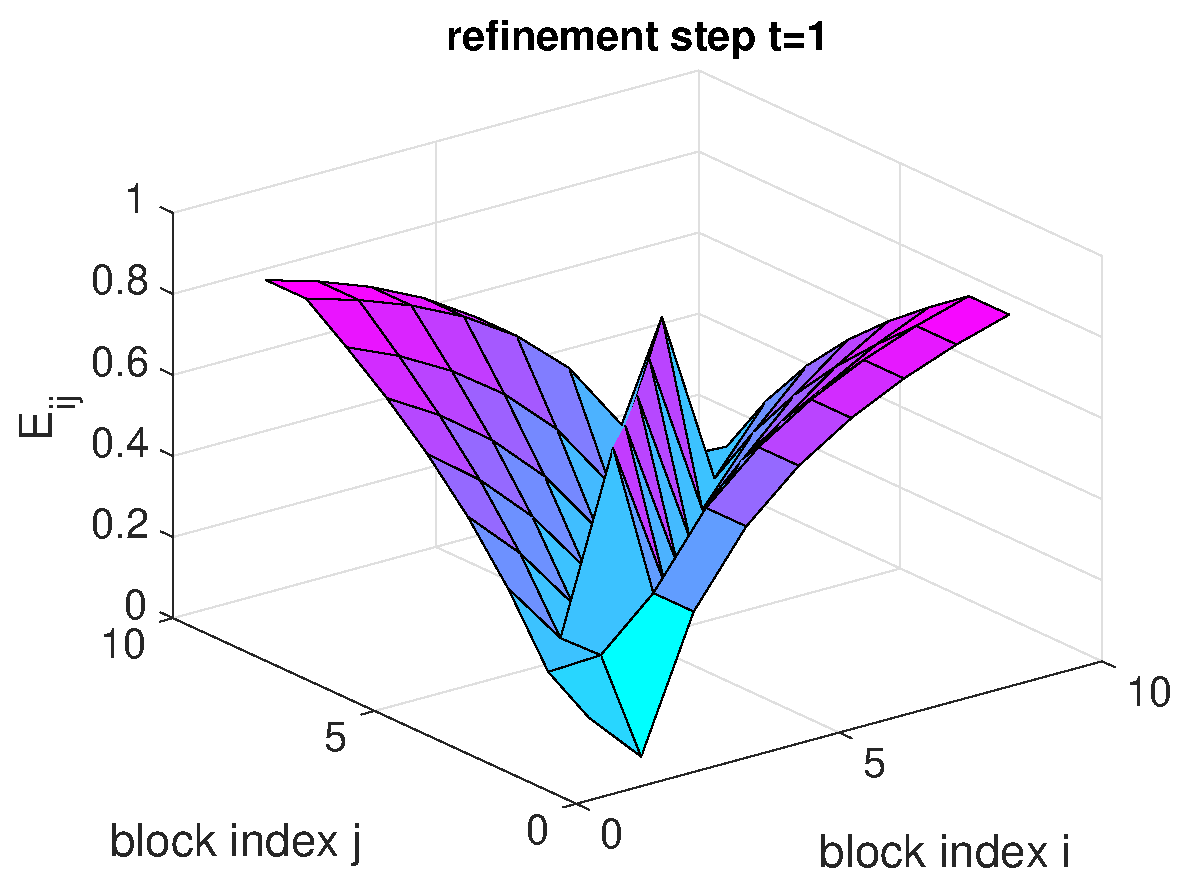
\includegraphics[width=0.475\linewidth]{figures/9times9_Z1_Error_t1.eps}
% 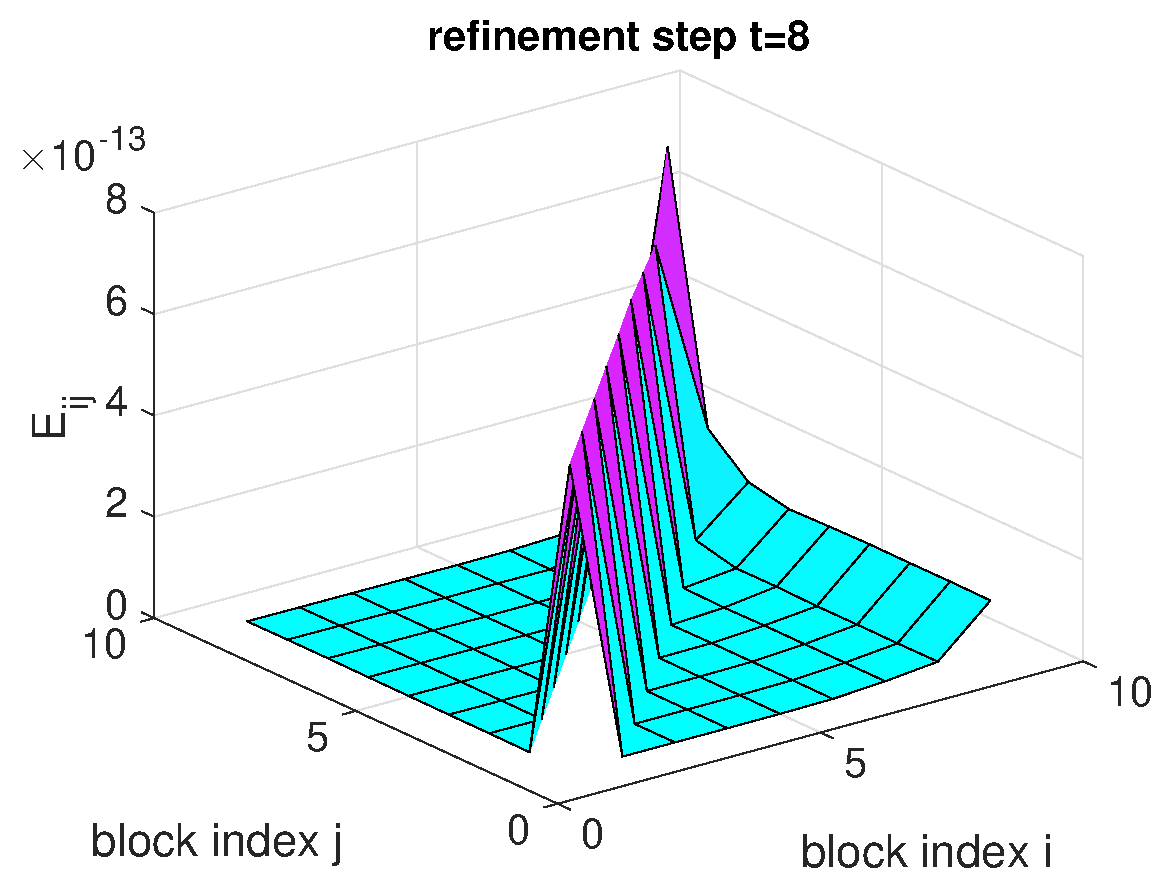
\includegraphics[width=0.475\linewidth]{figures/9times9_Z1_Error_t8.eps}\\[1ex]
% 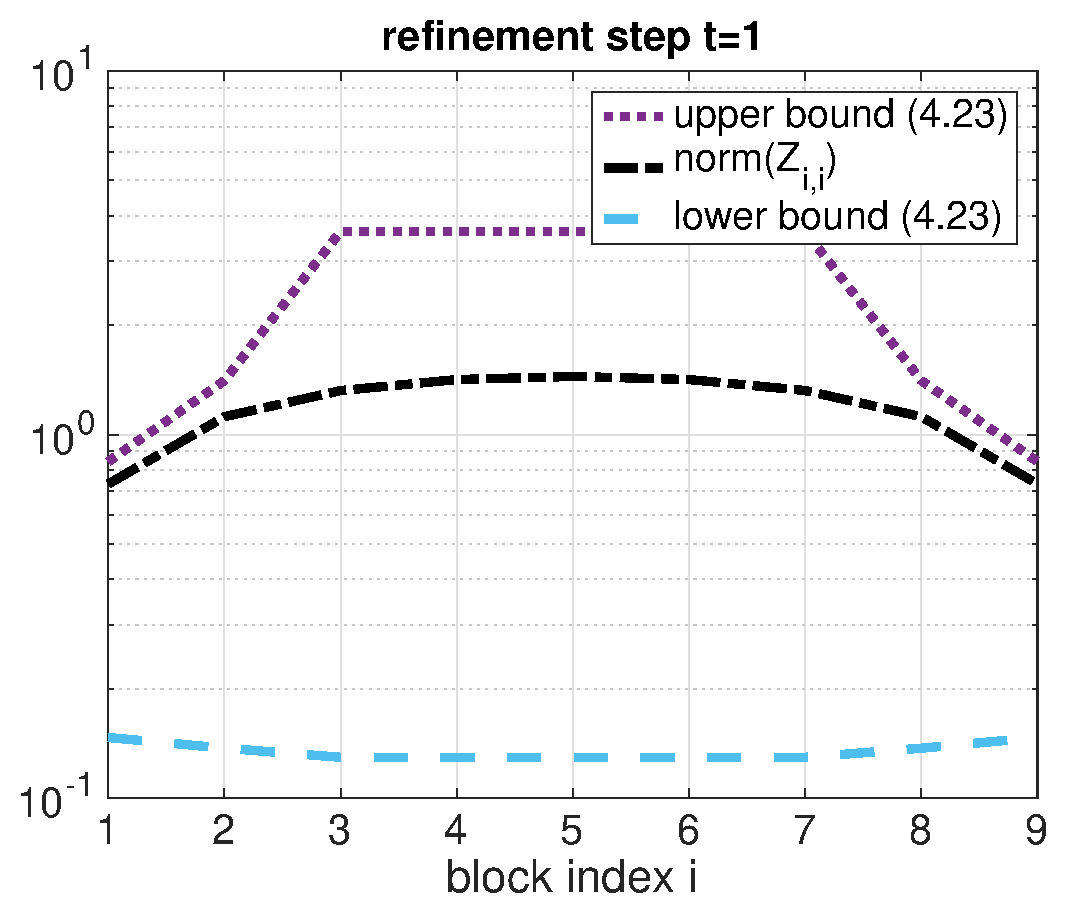
\includegraphics[width=0.475\linewidth]{figures/9times9_Z1_Bounds_t1.eps}
% 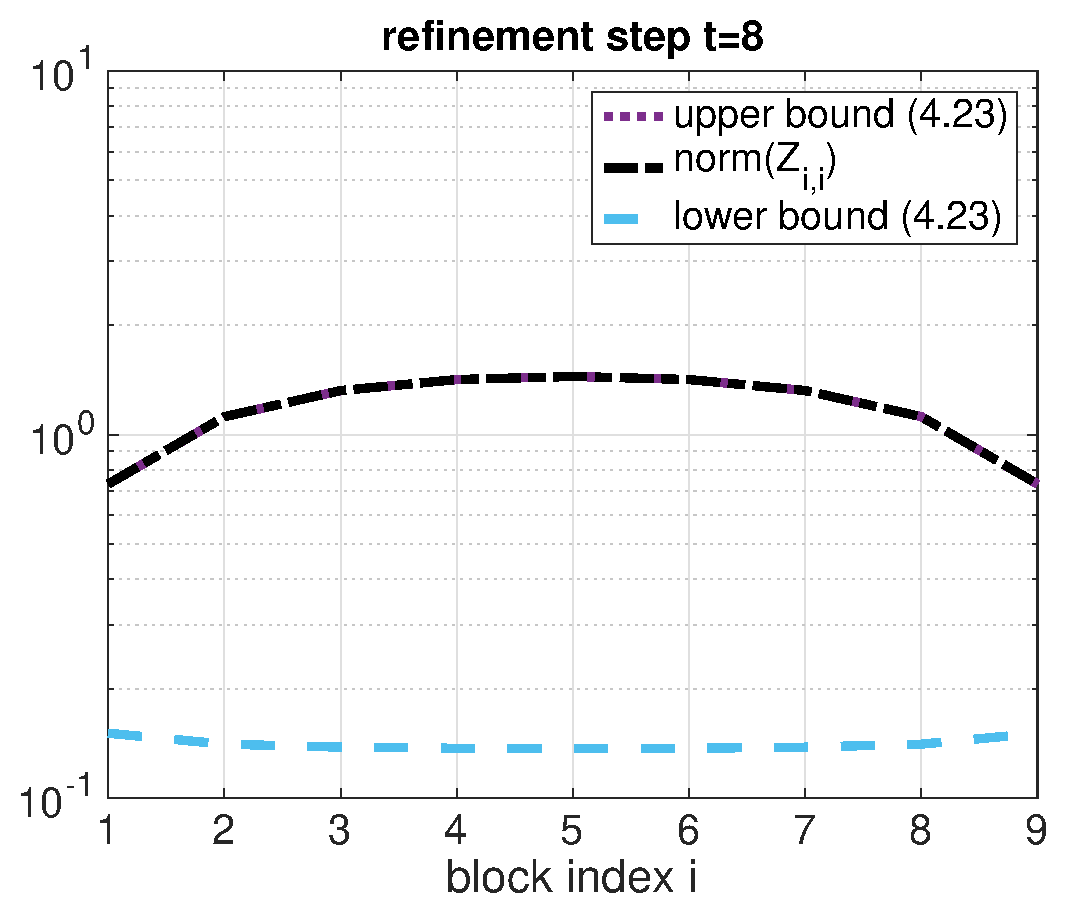
\includegraphics[width=0.475\linewidth]{figures/9times9_Z1_Bounds_t8.eps}
% %\includegraphics[width=0.475\linewidth]{figures/9times9_Z1_up-off-Bounds.eps}
% %\includegraphics[width=0.475\linewidth]{figures/9times9_Z1_low-off-Bounds.eps}
% \caption{Relative errors $\E^{\text{u}}_{ij}$ (top row), upper and lower bounds on $\|\Z_{ii}\|_2$ (bottom row) for the matrix $A$ of Example~\ref{ex:BDiDo:symm}.}
% \label{fig:BDiDo:ex:symm}
% \end{figure}
%
\begin{figure}[h!]
\vspace{-0.9em}
\hspace{-1cm}
\centering
\hspace*{2em}
\begin{minipage}[t]{0.48\linewidth}
\centering
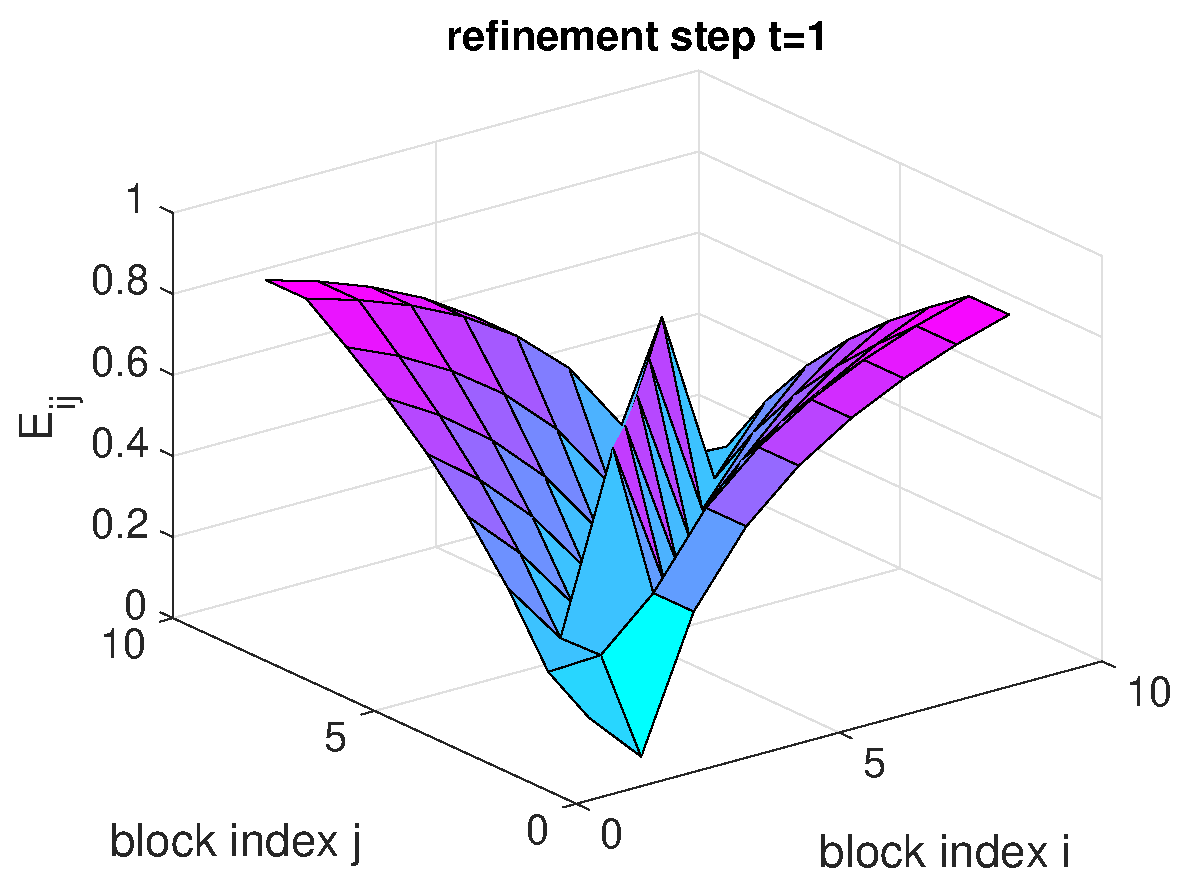
\includegraphics[width=0.99\linewidth]{figures/9times9_Z1_Error_t1.eps}
\end{minipage}
%
\begin{minipage}[t]{0.48\linewidth}
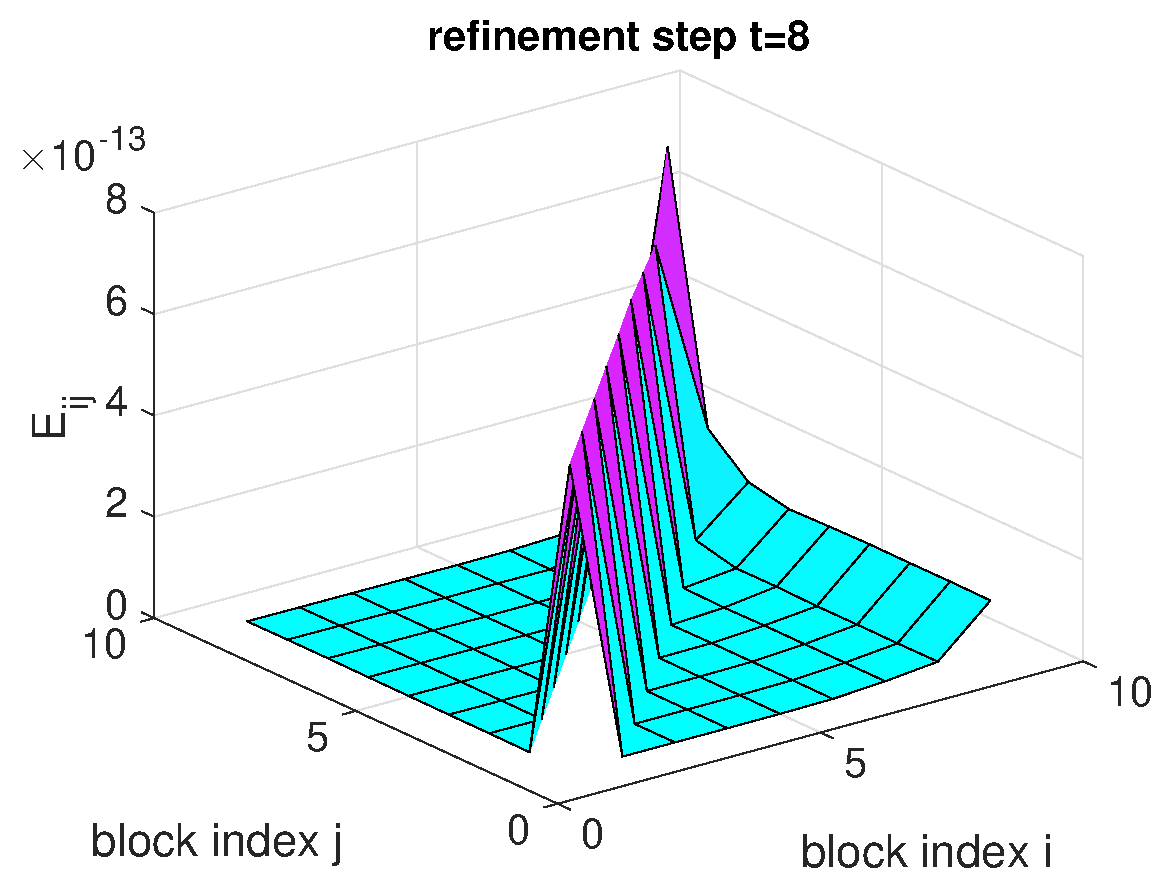
\includegraphics[width=0.99\linewidth]{figures/9times9_Z1_Error_t8.eps}
\end{minipage}
\\\vspace*{0.8em}
\begin{minipage}[t]{0.48\linewidth}
\centering
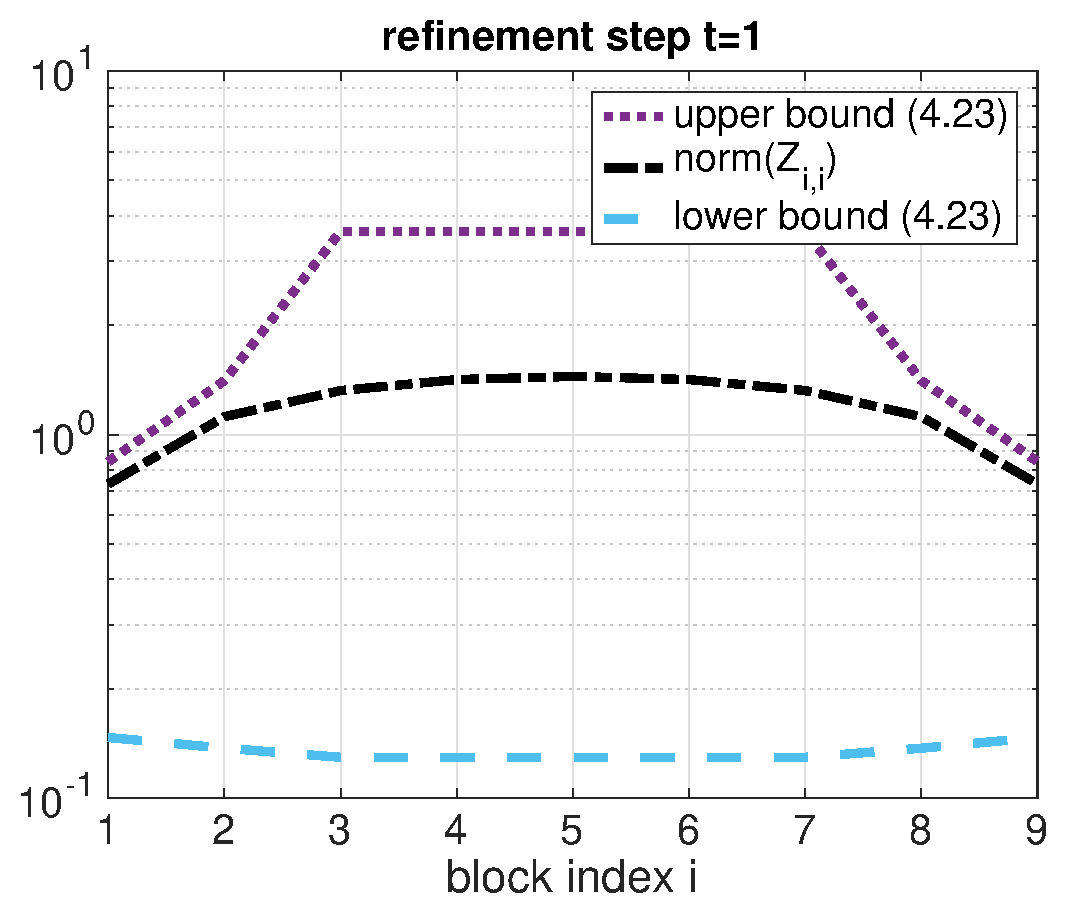
\includegraphics[width=0.99\linewidth]{figures/9times9_Z1_Bounds_t1.eps}
\end{minipage}
%
\begin{minipage}[t]{0.48\linewidth}
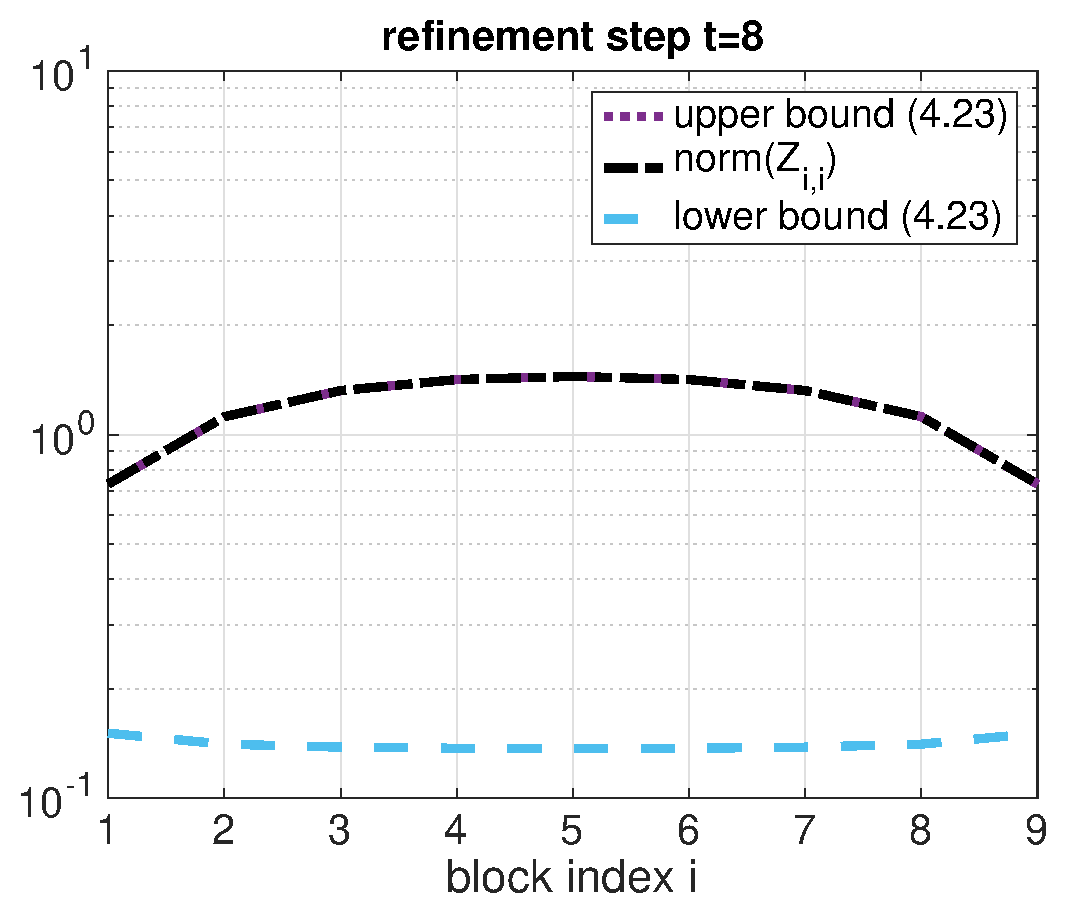
\includegraphics[width=0.99\linewidth]{figures/9times9_Z1_Bounds_t8.eps}
\end{minipage}
\caption{Relative errors $\E^{\text{u}}_{ij}$ (top row), upper and lower bounds on $\|\Z_{ii}\|_2$ (bottom row) for the matrix $A$ of Example~\ref{ex:BDiDo:symm}.}
\label{fig:BDiDo:ex:symm}
\end{figure}
}% textrm
\end{example}

\newpage
\begin{example}\label{ex:BDiDo:nonsym1}{\textrm
Let $\A$ be the nonsymmetric block Toeplitz matrix of the form
\eqref{eq:BDiDo:kronA} with
$\T=\textnormal{tridiag}(-110,209.999,-99.999)\in\mathbb{R}^{9\times 9}$, i.e.,
$\A$ again takes the form \eqref{eq:BDiDo:blocktridiag} with
$\A_i=\textnormal{tridiag}(-110,419.999,-99.999)$,
$\B_i=\textnormal{diag}(-110)$, and $\C_i=\textnormal{diag}(-99.999)$. The
condition number in this case is $\kappa_2(\A)=57.5725$,  and for the computed
matrix $\Z$ we obtain $\|\Z\A-\I\|_2=1.5151\times 10^{-10}$.

The top row of \textnormal{Figure~\ref{fig:BDiDo:ex:nonsym1}} shows the
relative errors for the refinement steps $t=1$ and $t=8$. We observe that for
this nonsymmetric example the upper bounds are not as accurate as those given
in the symmetric case, producing a maximal relative error at refinement step
$t=8$ on the order $10^{-3}$. The bottom row of
\textnormal{Figure~\ref{fig:BDiDo:ex:nonsym1}} shows the upper and lower bounds
\eqref{eq:BDiDo:diagboundsiter} as well as the values $\|\Z_{ii}\|_2$ for
$i=1,\dots,9$, and refinement steps $t=1$ and $t=8$. Again we can observe that
while we obtain a reasonable approximation in the upper bounds on
$\|\Z_{ii}\|_2$ for $t=8$, the lower bounds almost do not improve by
the iterative refinement process. The maximal relative errors in the upper and
lower bounds and all refinement steps is shown in the following table:
%
%The maximal error of
%the lower bounds for the diagonal block entries of $Z$ in the maximal refinement step is again on the order %$10^{-1}$; see Table \ref{tab:errorA2}.
%
\begin{table}[h!]\scriptsize\centering
\begin{tabular}{c c c c c c c c c}
\hline
  t & 1 & 2 & 3 & 4 & 5 & 6 & 7 & 8 \\
$\max_{ij}\E^{u}_{ij}$ &  $0.88856$ & $ 0.70640$ & $0.46700$ &  $0.25859$ & $0.12442$ & $0.05378$ &  $0.02140$ &  $0.00824$\\
$\max_i \E^{l}_{i}$ & $0.90934$ & $0.90768$ & $0.90652$ & $0.90411$ & $0.90411$ & $0.90411$ &  $0.90411$ &  $0.90411$\\
\hline
\end{tabular}
%\caption{Values of the maximum relative errors for the matrix $A$ of Example 2.2 and  different values of $t$.}
%\label{tab:errorA2}
\end{table}
%\newpage
% \begin{figure}[h!]
% \centering
% % 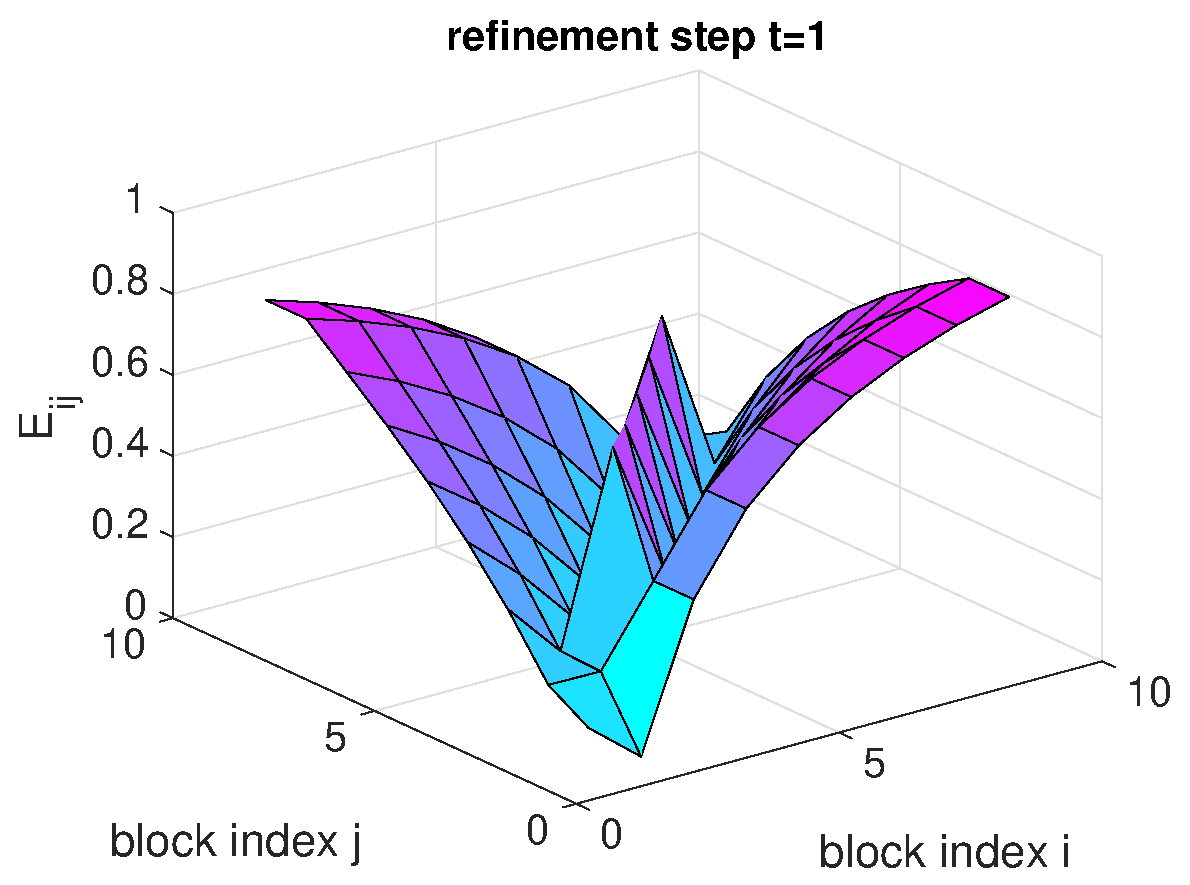
\includegraphics[width=0.475\linewidth]{figures/9times9_Z2_Error_t1.eps}
% % 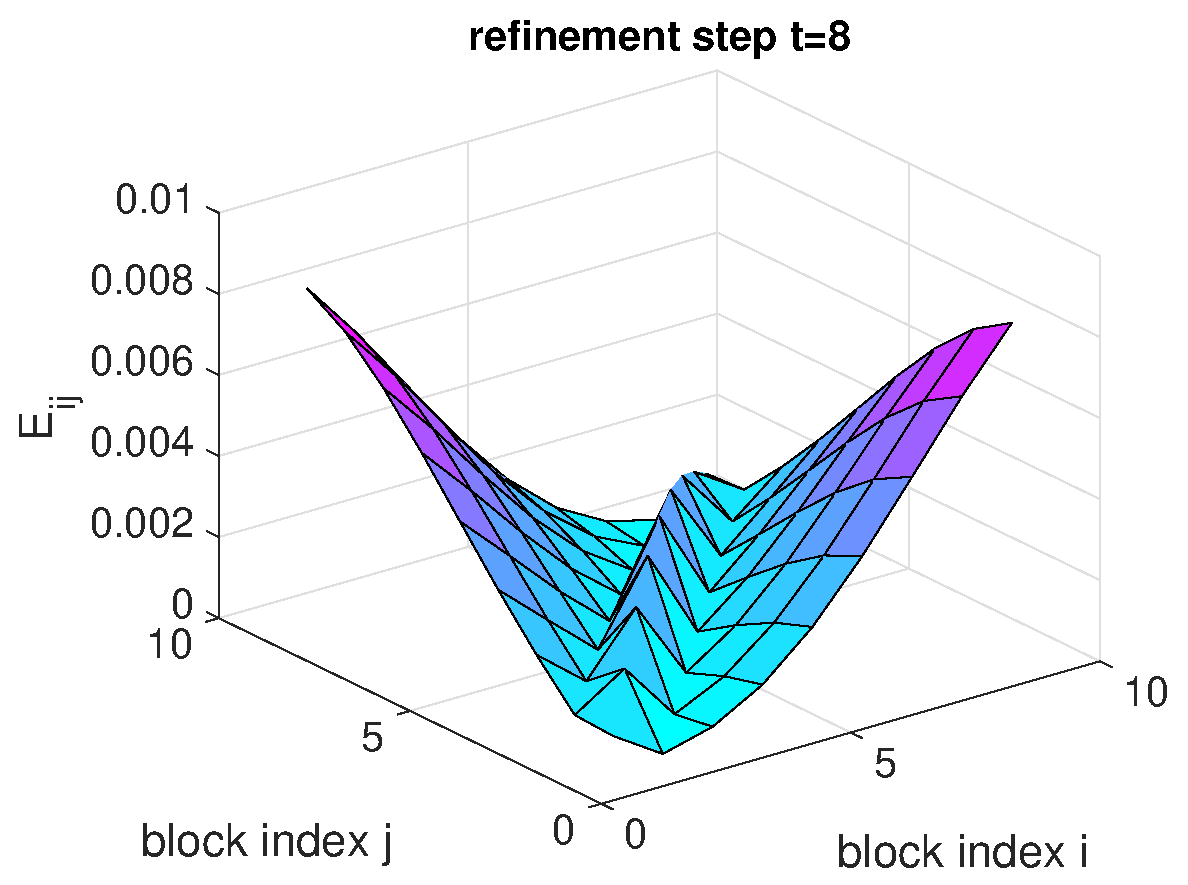
\includegraphics[width=0.475\linewidth]{figures/9times9_Z2_Error_t8.eps}\\[1ex]
% % 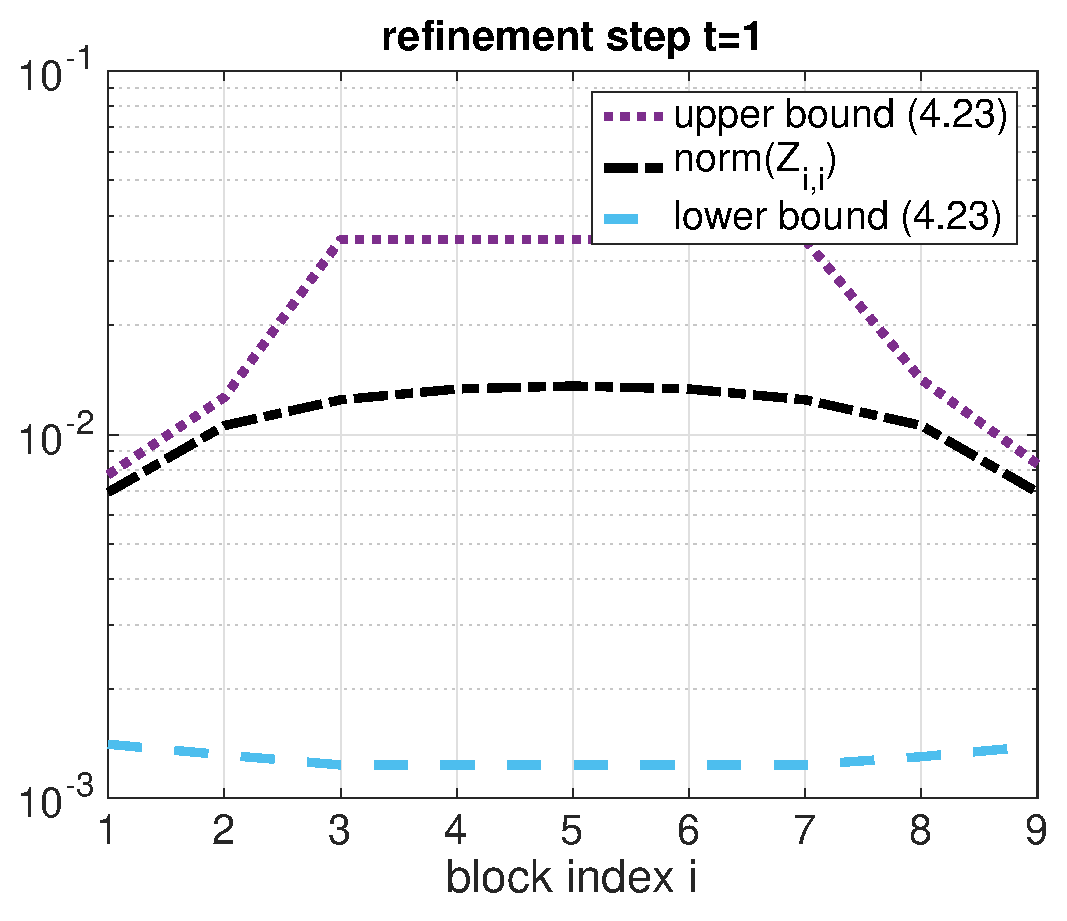
\includegraphics[width=0.475\linewidth]{figures/9times9_Z2_Bounds_t1.eps}
% % 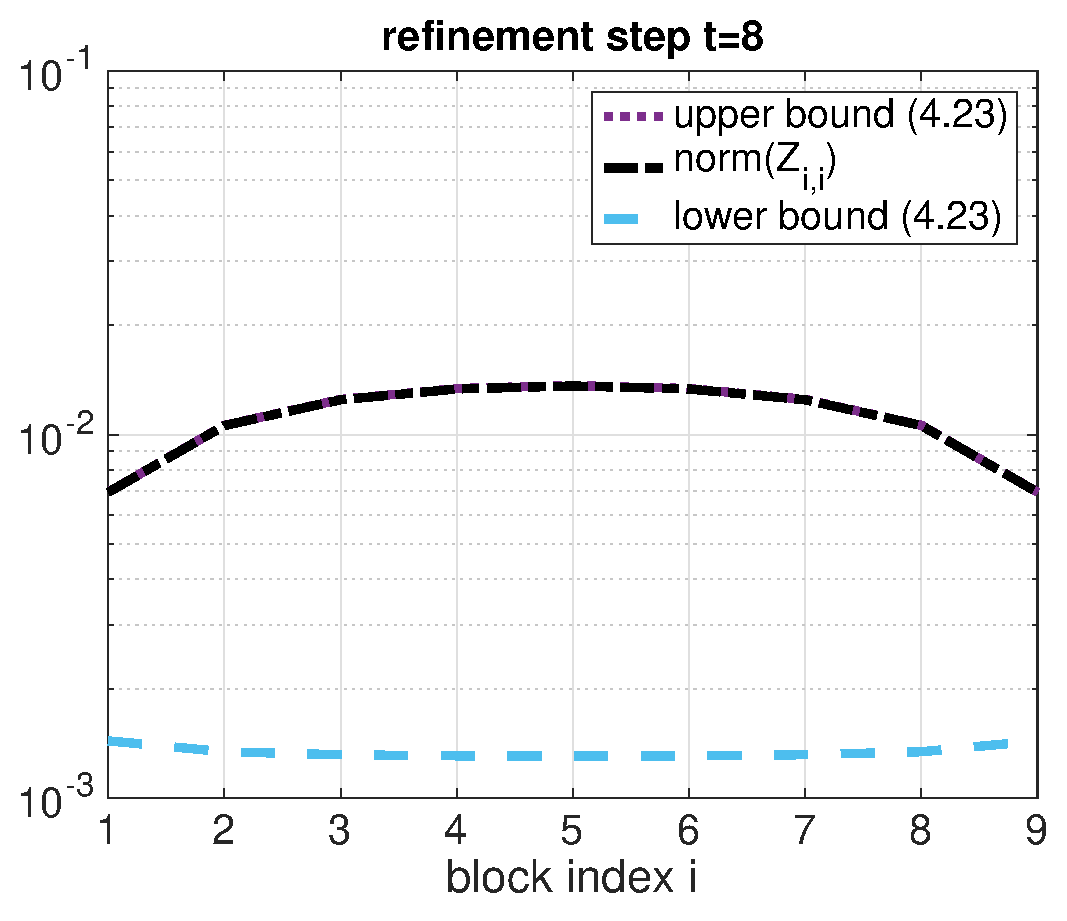
\includegraphics[width=0.475\linewidth]{figures/9times9_Z2_Bounds_t8.eps}
% 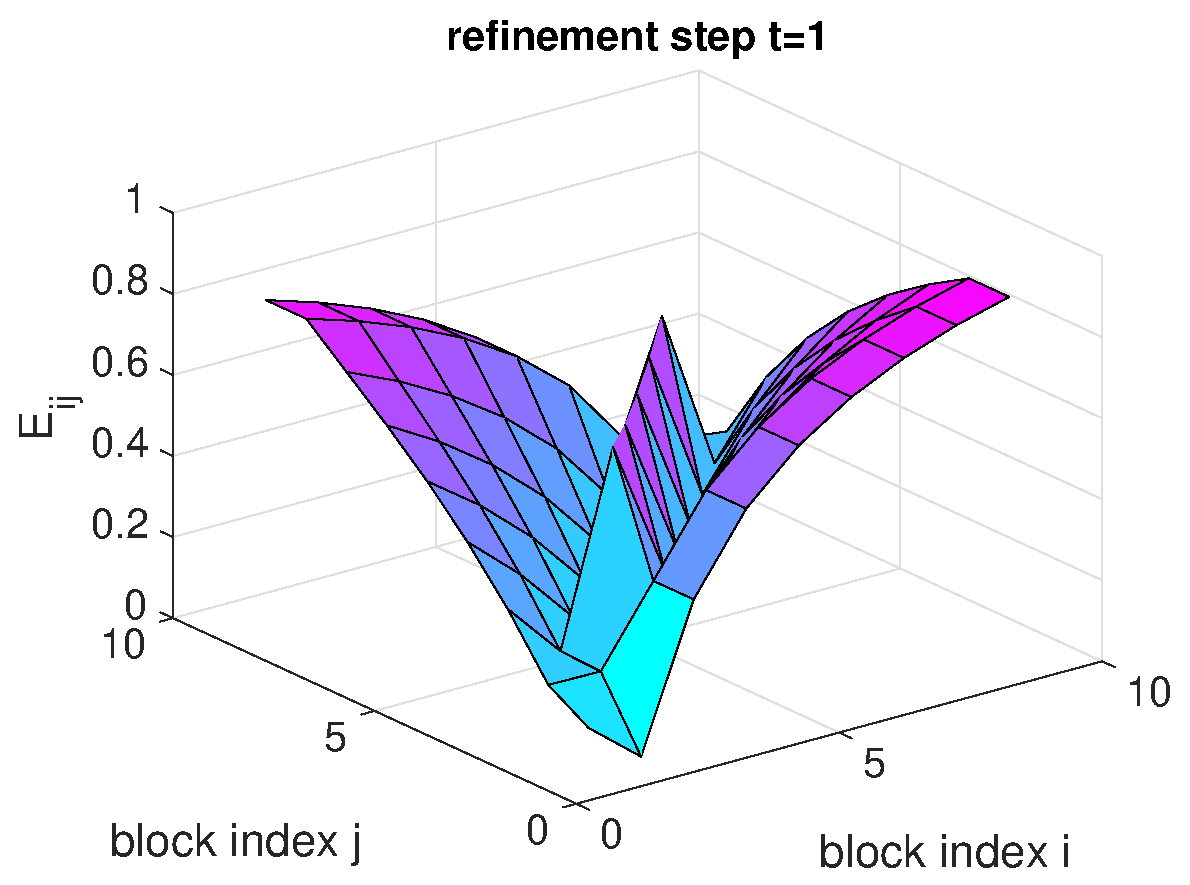
\includegraphics[scale=0.17]{figures/9times9_Z2_Error_t1.eps}
% 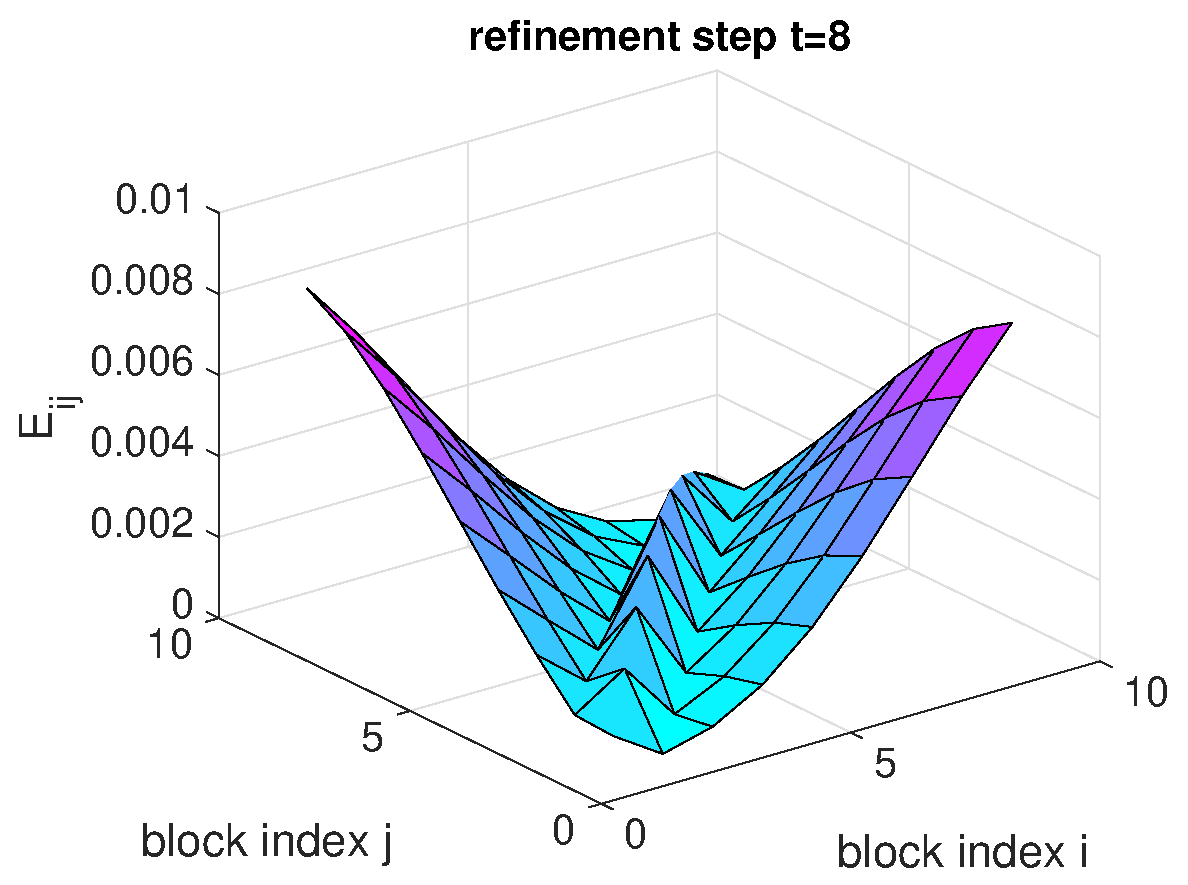
\includegraphics[scale=0.17]{figures/9times9_Z2_Error_t8.eps}\\[1ex]
% 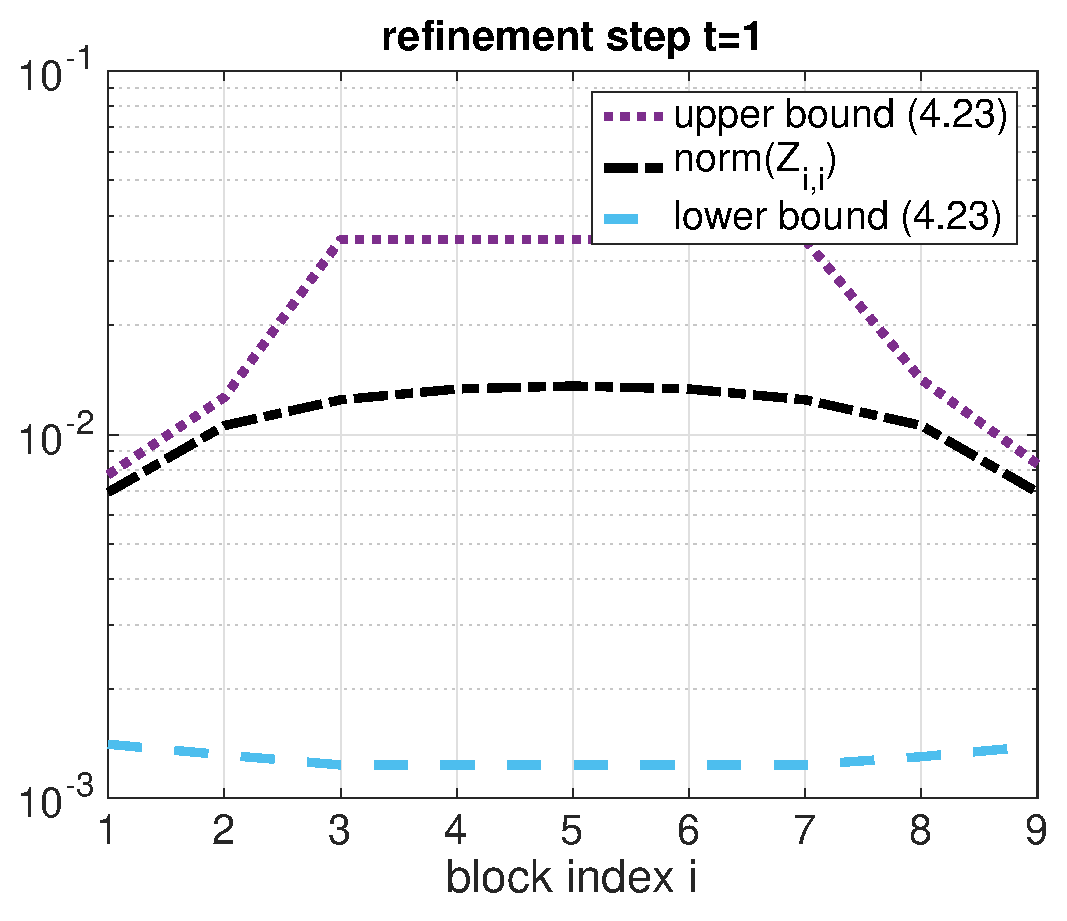
\includegraphics[scale=0.17]{figures/9times9_Z2_Bounds_t1.eps}
% 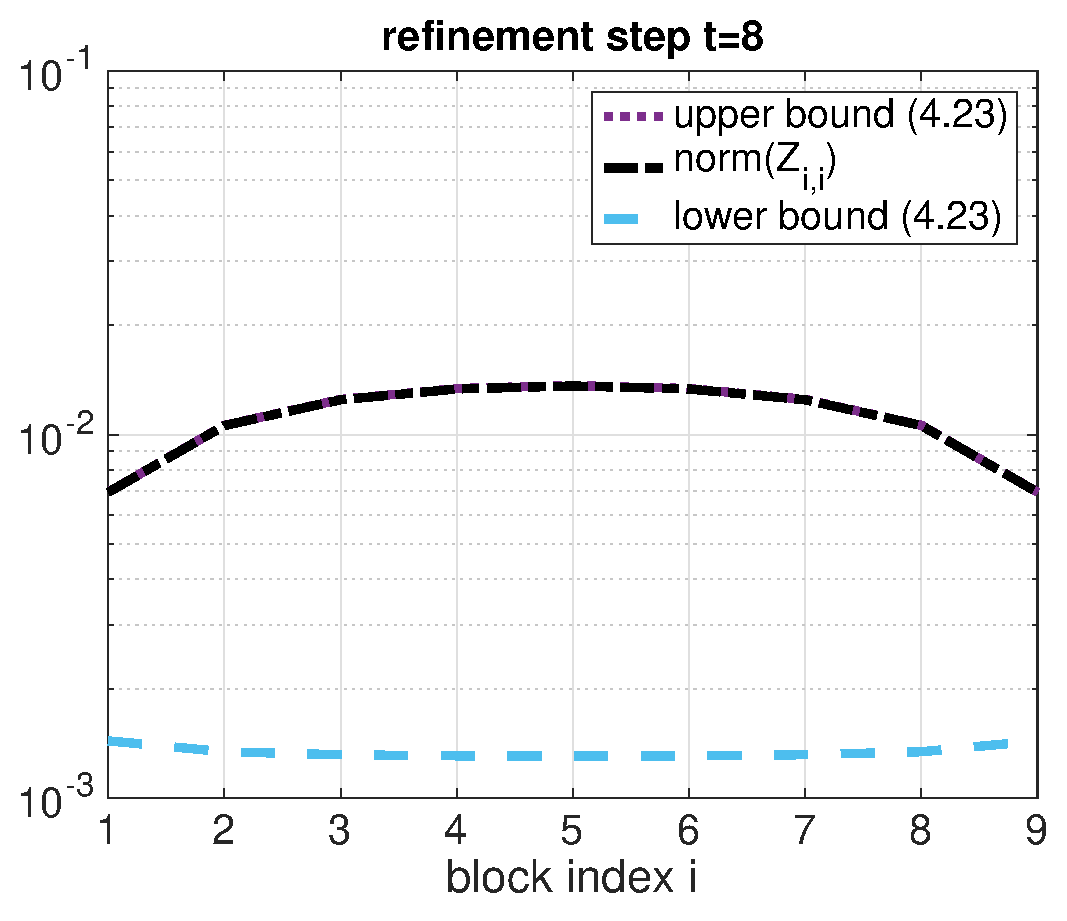
\includegraphics[scale=0.17]{figures/9times9_Z2_Bounds_t8.eps}
% \caption{Relative errors $\E^{\text{u}}_{ij}$ (top row), and upper and lower bounds on $\|\Z_{ii}\|_2$ (bottom row) for the matrix $\A$ of Example~\ref{ex:BDiDo:nonsym1}.}
% \label{fig:BDiDo:ex:nonsym1}
% \end{figure}
%
\begin{figure}[h!]
\vspace{-1.1em}
\hspace{-1cm}
\centering
\hspace*{2em}
\begin{minipage}[t]{0.48\linewidth}
\centering
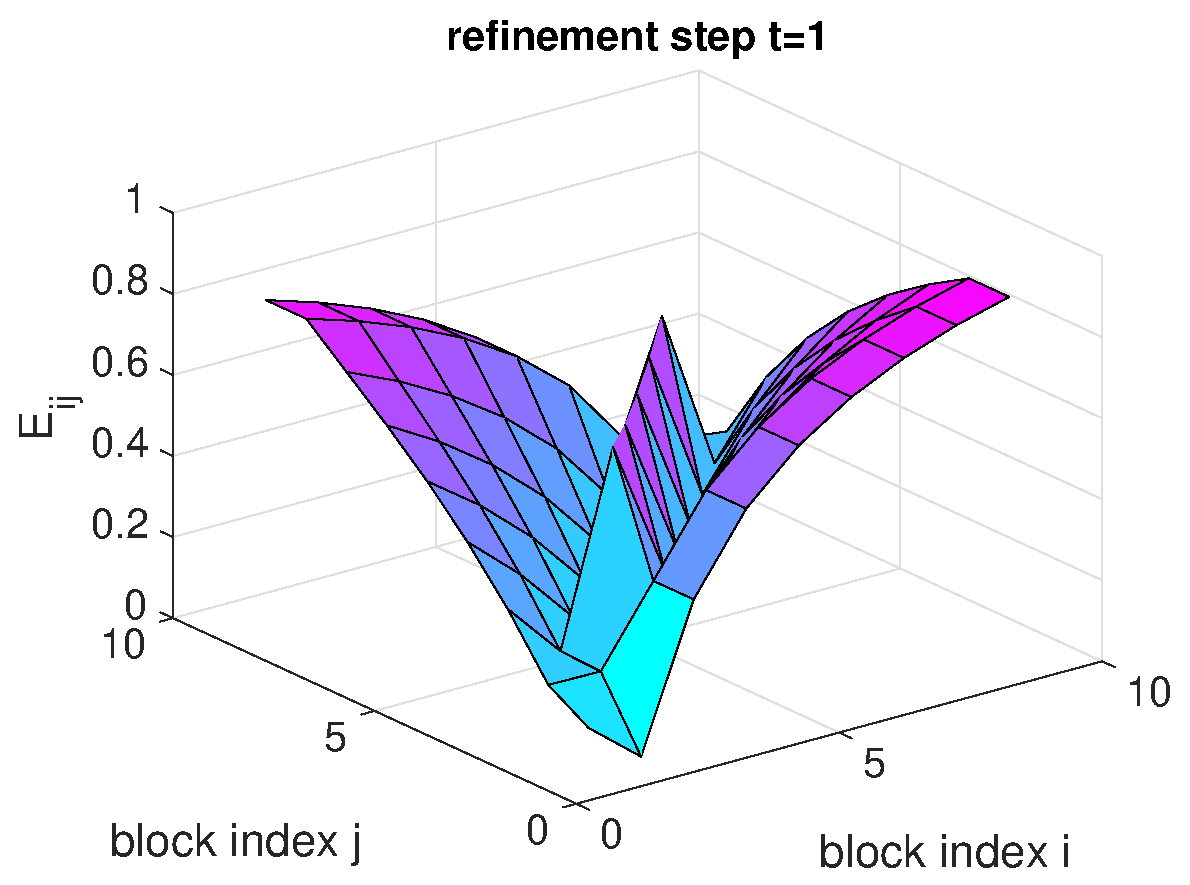
\includegraphics[width=0.99\linewidth]{figures/9times9_Z2_Error_t1.eps}
\end{minipage}
%
\begin{minipage}[t]{0.48\linewidth}
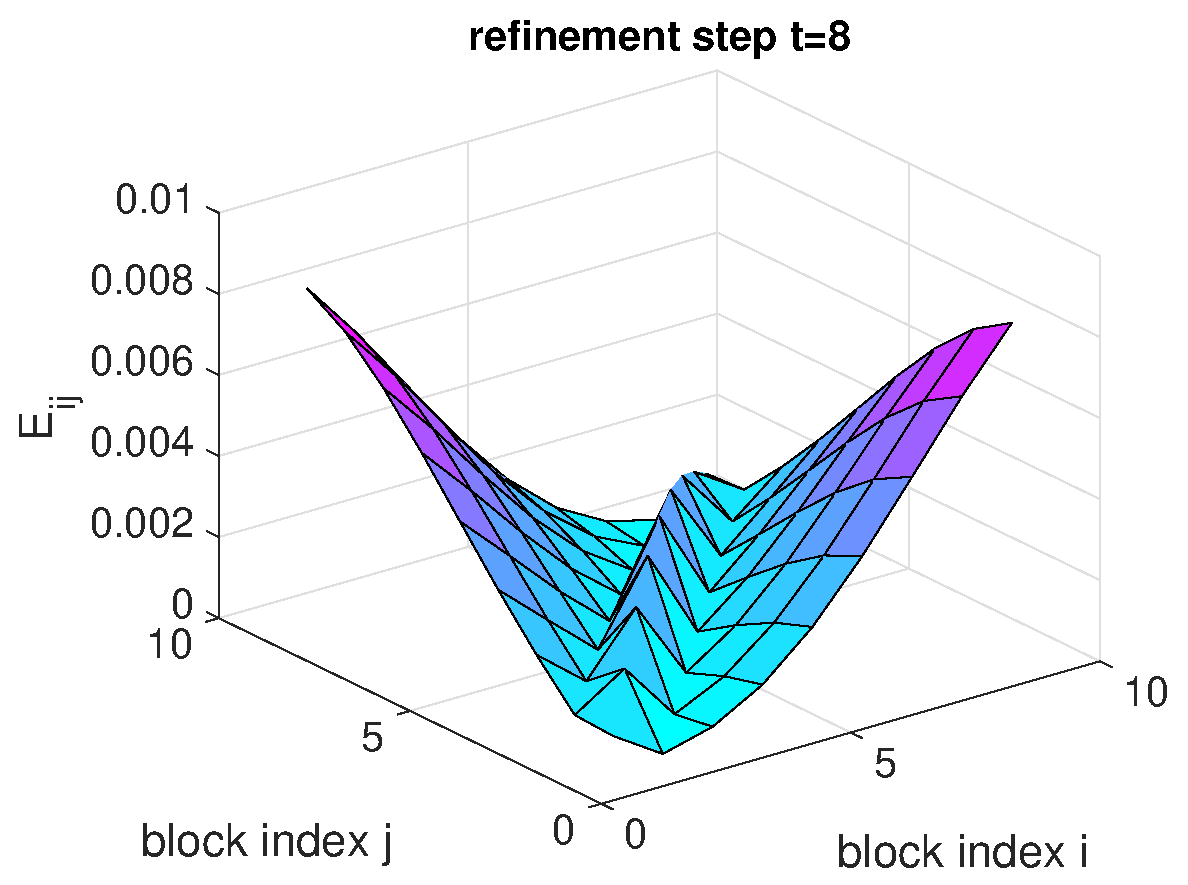
\includegraphics[width=0.99\linewidth]{figures/9times9_Z2_Error_t8.eps}
\end{minipage}
\\%\vspace*{0.1em}
\begin{minipage}[t]{0.48\linewidth}
\centering
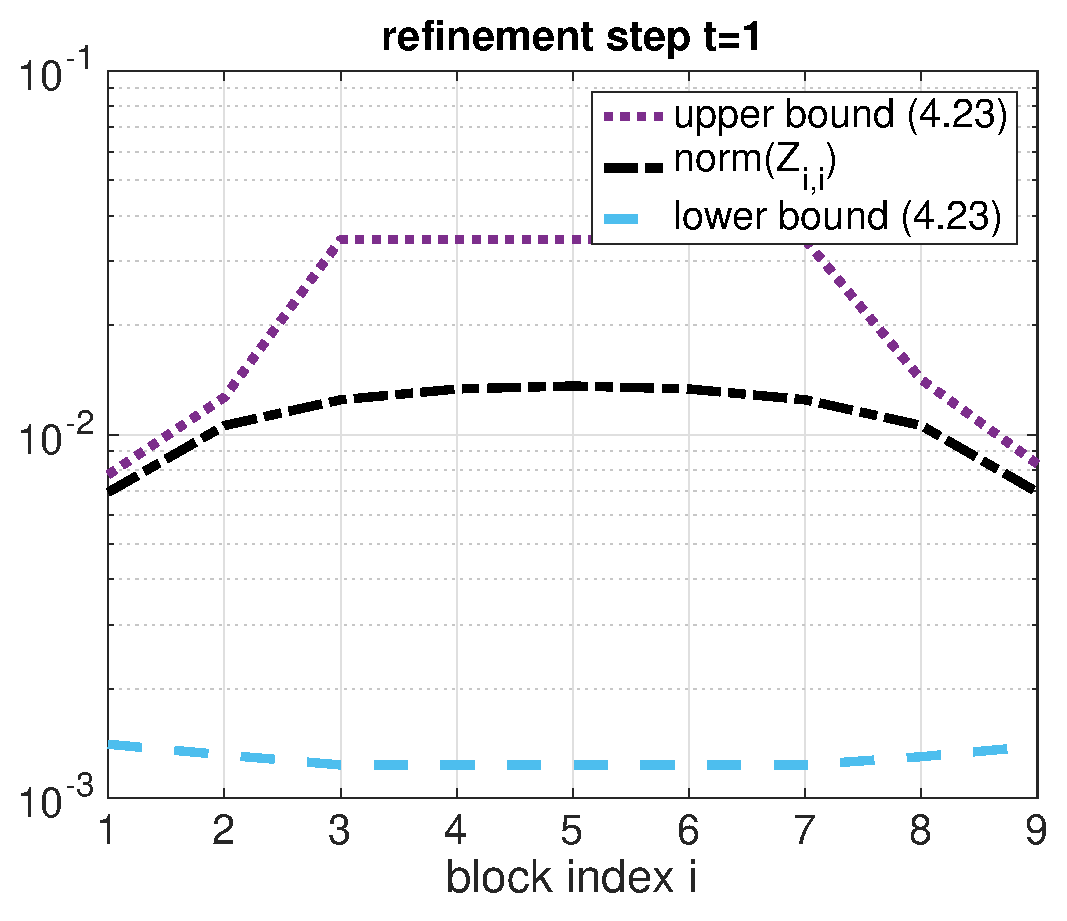
\includegraphics[width=0.99\linewidth]{figures/9times9_Z2_Bounds_t1.eps}
\end{minipage}
%
\begin{minipage}[t]{0.48\linewidth}
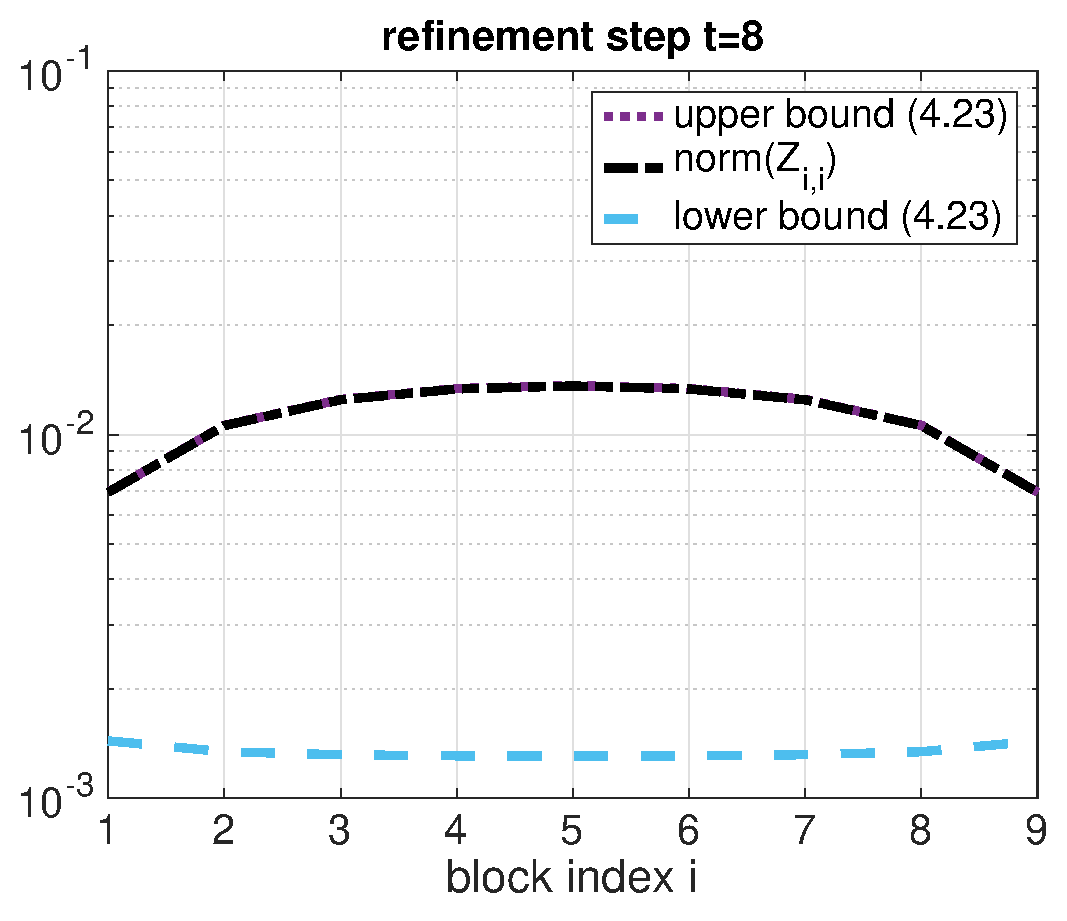
\includegraphics[width=0.99\linewidth]{figures/9times9_Z2_Bounds_t8.eps}
\end{minipage}
\caption{Relative errors $\E^{\text{u}}_{ij}$ (top row), and upper and lower bounds on $\|\Z_{ii}\|_2$ (bottom row) for the matrix $\A$ of Example~\ref{ex:BDiDo:nonsym1}.}
\label{fig:BDiDo:ex:nonsym1}
\end{figure}
}\end{example}

\newpage

\begin{example}\label{ex:BDiDo:nonsym2}{\textrm
We now consider the  nonsymmetric block tridiagonal matrix
\[\A~=(\R\otimes \I)(\T\otimes \I+ \I\otimes~\T) \;\;\in\;\;\mathbb{R}^{81\times 81},\]
where $\T$ is given as in \textnormal{Example~\ref{ex:BDiDo:symm}}, and
$\R\in\mathbb{R}^{9\times 9}$ is a random diagonal matrix with nonzero integer
entries between $0$ and $10$ and constructed in \textnormal{\texttt{MATLAB}}
with the command \textnormal{\texttt{\R = diag(ceil(10*rand(9,1)))}}. Thus,
$\A$ is of the form \eqref{eq:BDiDo:blocktridiag} with random tridiagonal
Toeplitz matrices $\A_i$, and random constant diagonal matrices $\B_i$ and
$\C_i$ for all $i$. For this matrix we have $\kappa_2(\A)=489.7595$, and the
computed matrix $\Z$ yields $\|\Z\A-\I\|_2=2.8328\times 10^{-10}$. The relative
errors in the bounds are shown in \textnormal{Figure~\ref{fig:BDiDo:ex:nonsym2}} and in the following table:
%
\begin{table}[h!]\scriptsize\centering
\begin{tabular}{c c c c c c c c c}
\hline
%\cline{2-5}
 t & 1 & 2 & 3 & 4 & 5 & 6 & 7 & 8 \\
 $\max_{ij}\E^{u}_{ij}$ &  $0.84477$ & $0.63381$  &  $0.39537$ &  $0.20898$ & $0.09595$ &  $0.03780$ &  $0.01109$ &  $9.739\times 10^{-13}$\\
 $\max_{i}\E^{l}_{i}$ &  $0.91039$ & $0.90877$ & $0.90765$ & $0.90529$ & $0.90529$ &  $0.90529$ &  $0.90529$ &  $0.90529$\\
  \hline
\end{tabular}
%\caption{Values of the maximum relative errors for the matrix $A$ of Example 2.3 and  different values of $t$.}
%\label{tab:errorA3}
\end{table}
%

%\newpage
% \begin{figure}[h!]
% \centering
% % 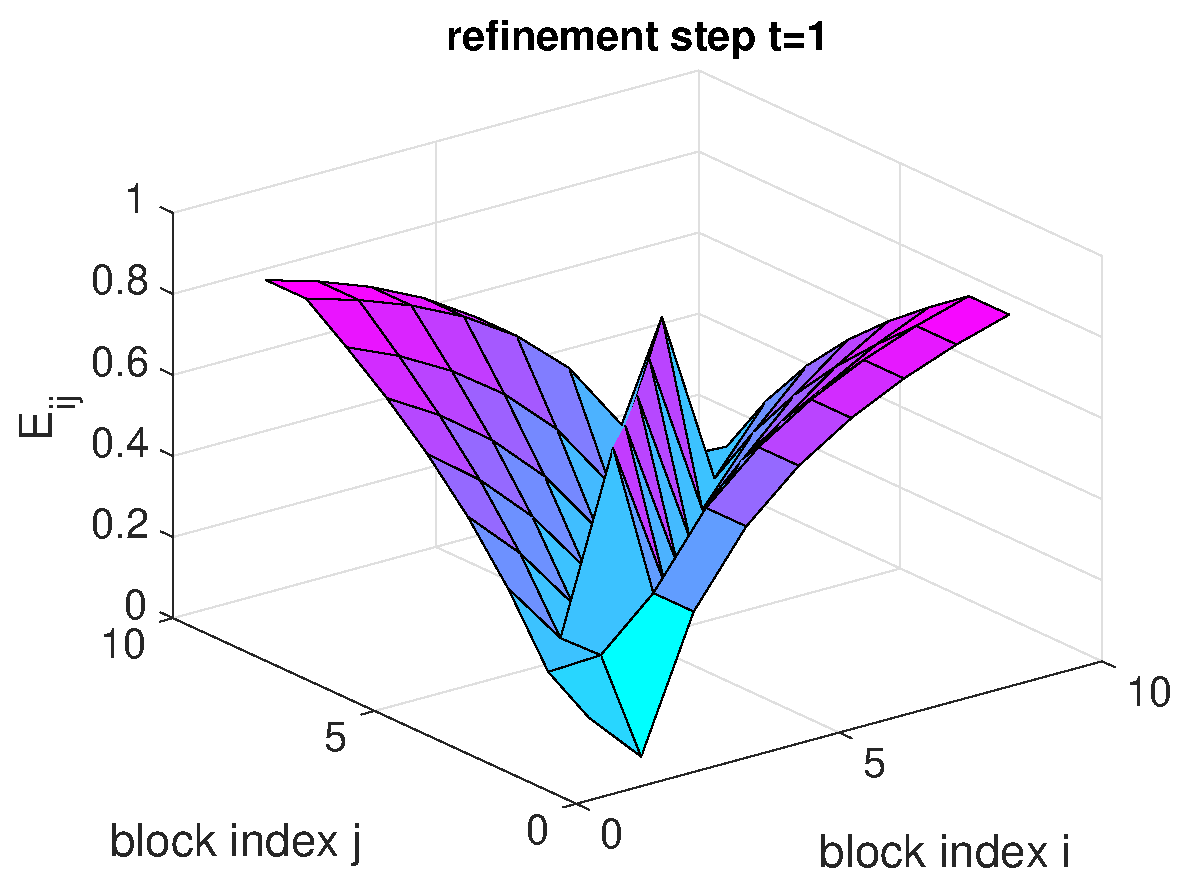
\includegraphics[width=0.475\linewidth]{figures/9times9_Z3_Error_t1.eps}
% % 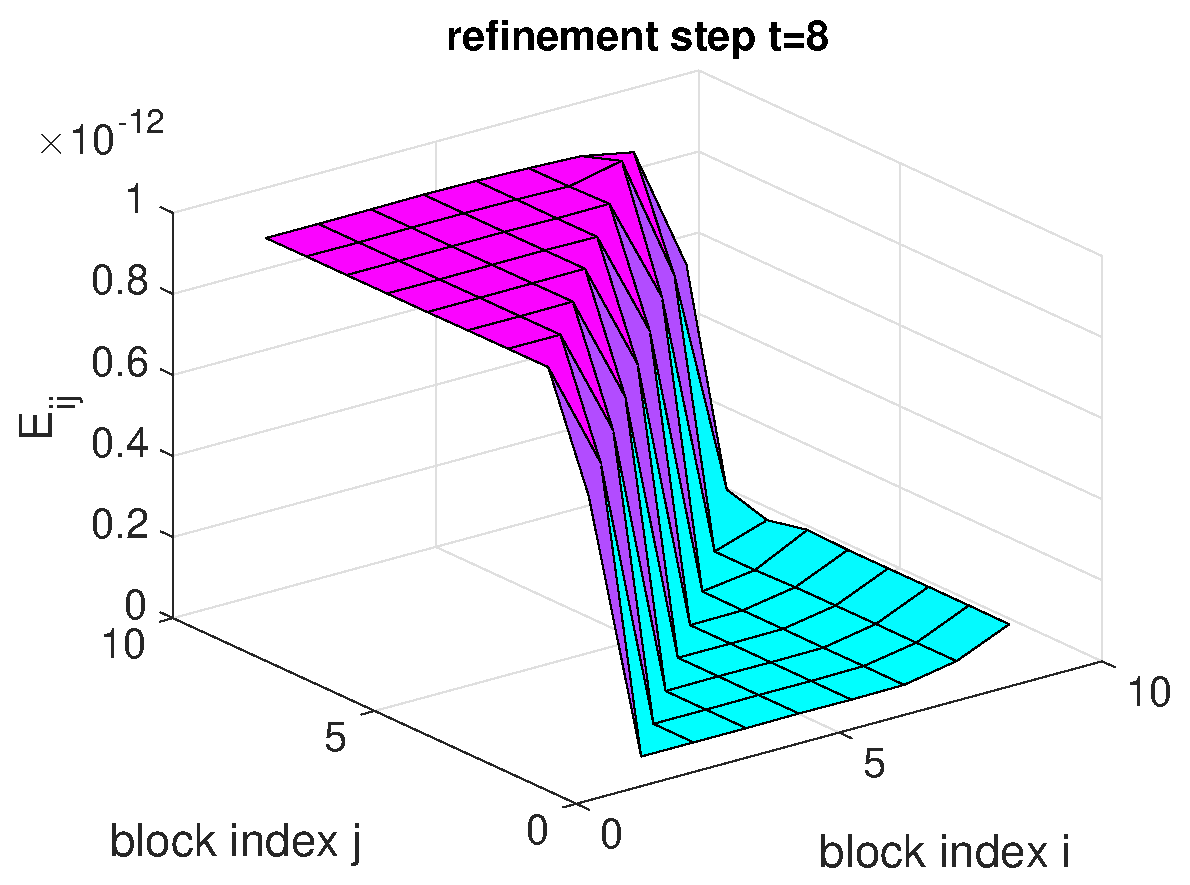
\includegraphics[width=0.475\linewidth]{figures/9times9_Z3_Error_t8.eps}\\[1ex]
% % 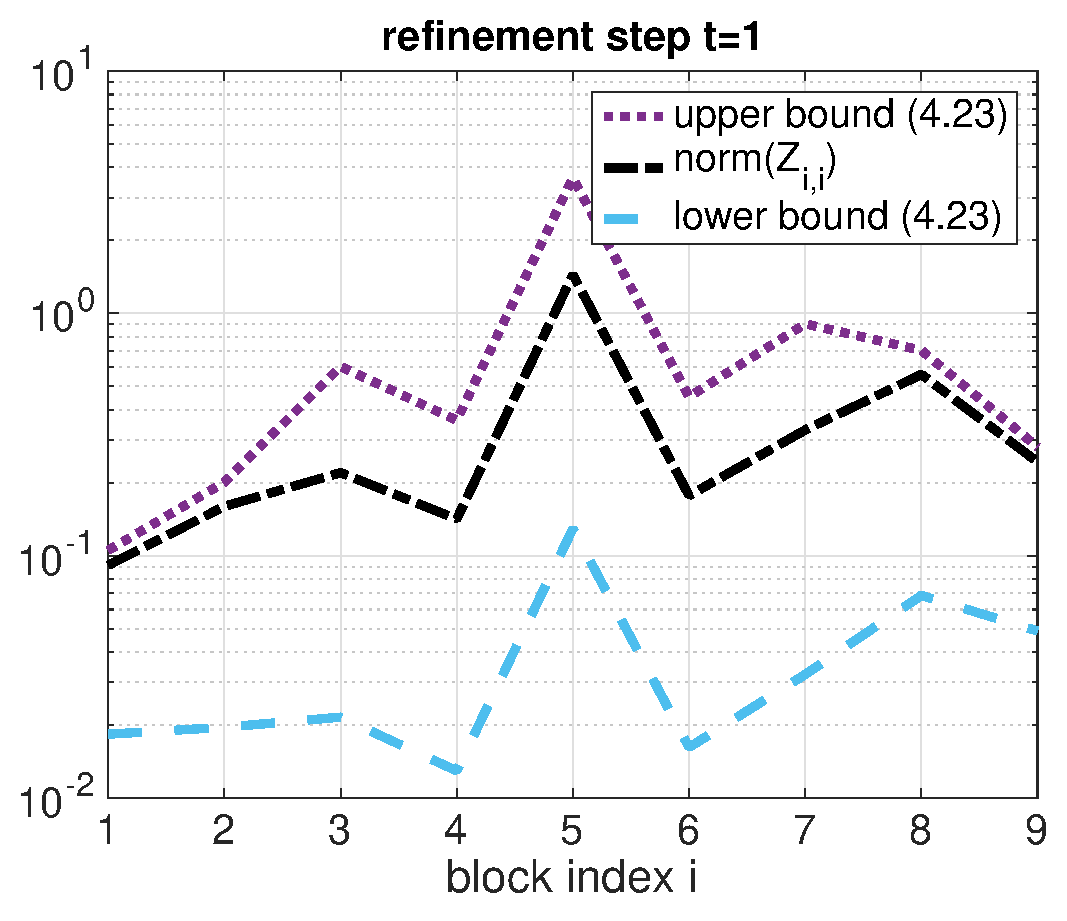
\includegraphics[width=0.475\linewidth]{figures/9times9_Z3_Bounds_t1.eps}
% % 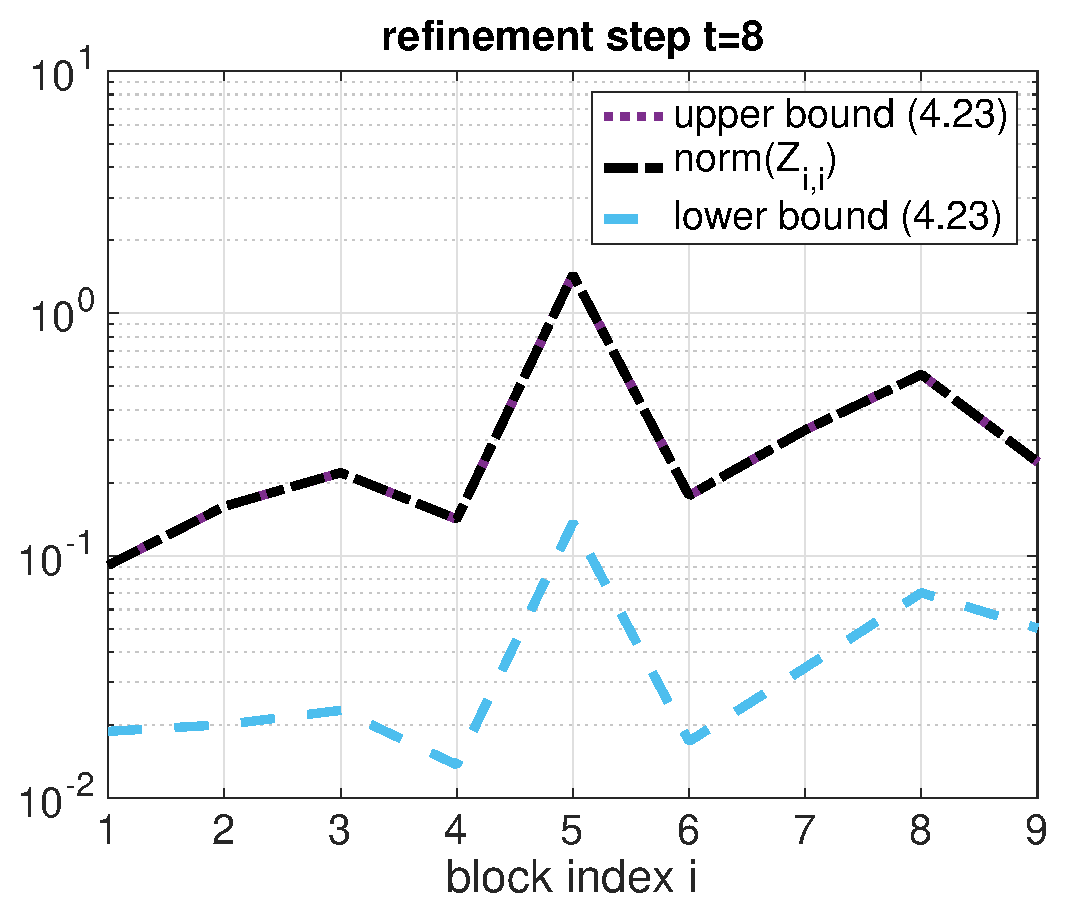
\includegraphics[width=0.475\linewidth]{figures/9times9_Z3_Bounds_t8.eps}
% 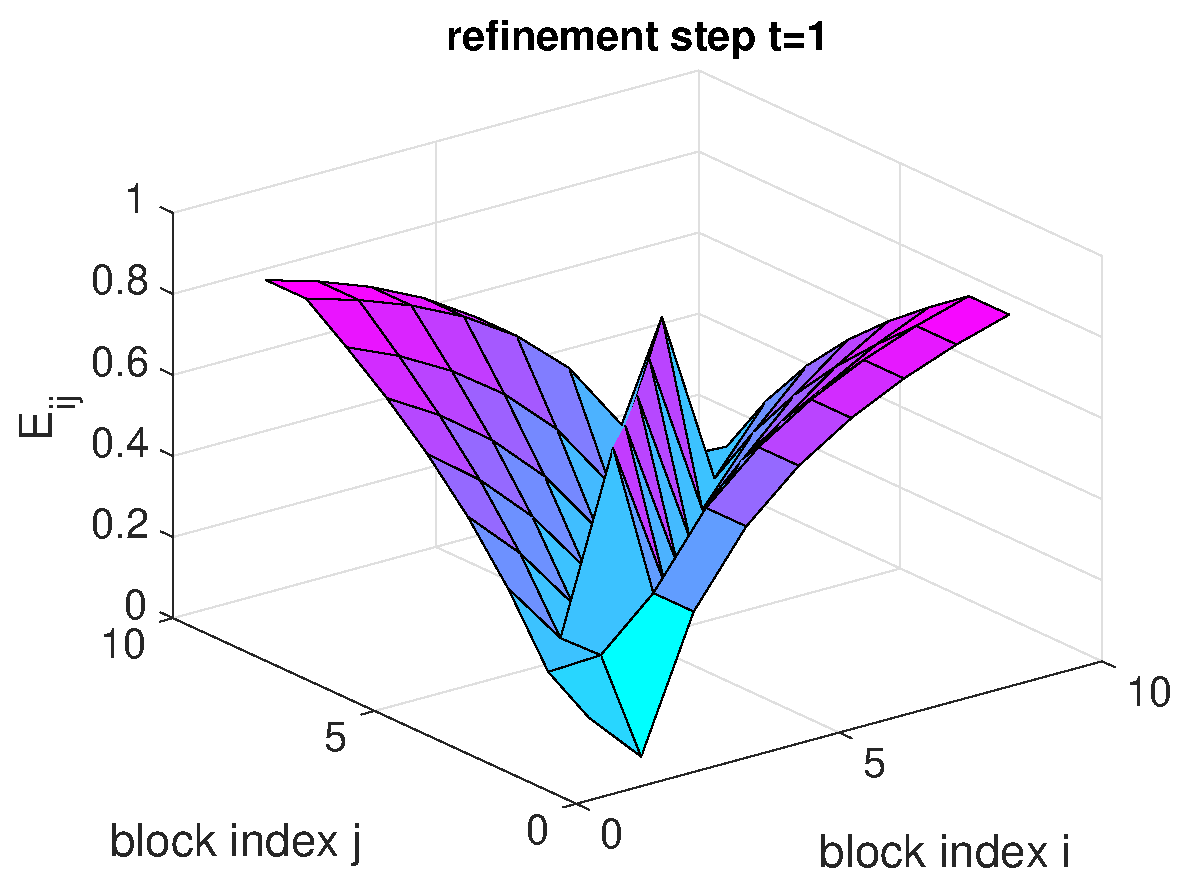
\includegraphics[scale=0.18]{figures/9times9_Z3_Error_t1.eps}
% 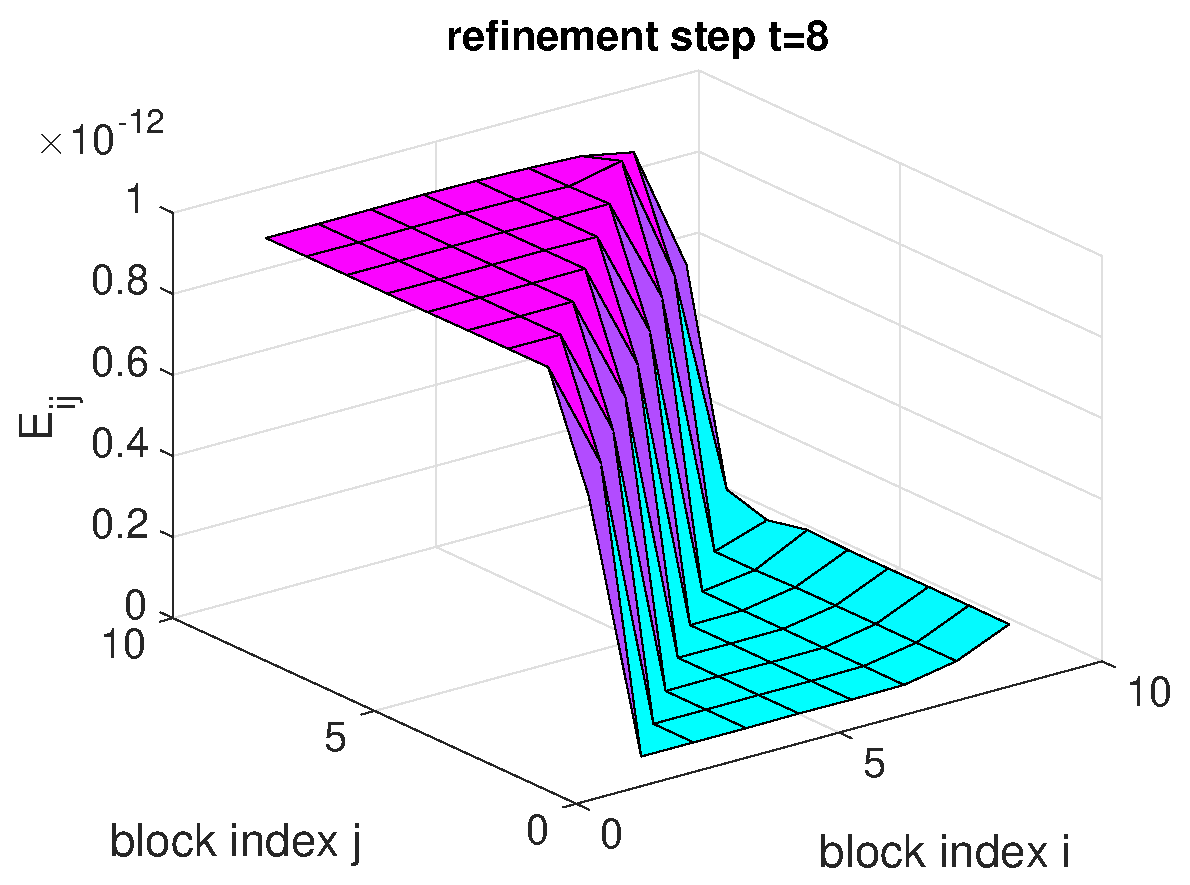
\includegraphics[scale=0.18]{figures/9times9_Z3_Error_t8.eps}\\[1ex]
% 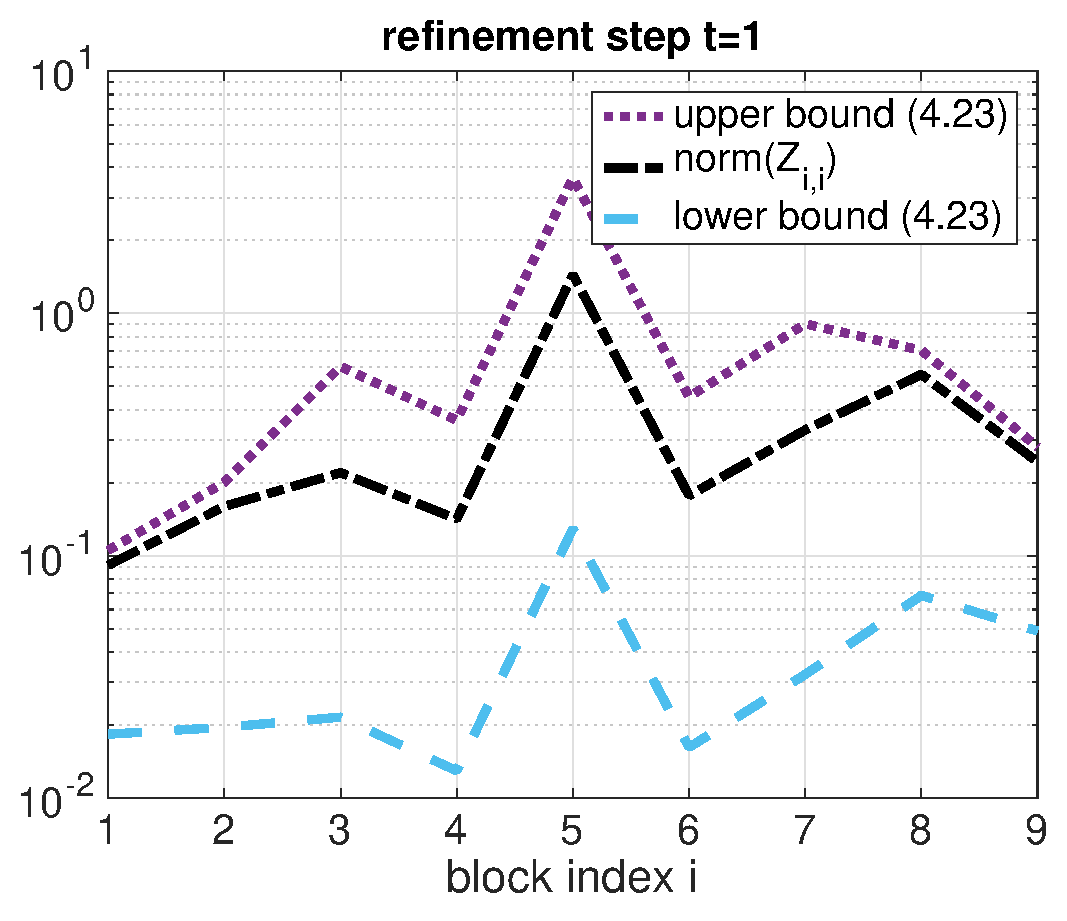
\includegraphics[scale=0.18]{figures/9times9_Z3_Bounds_t1.eps}
% 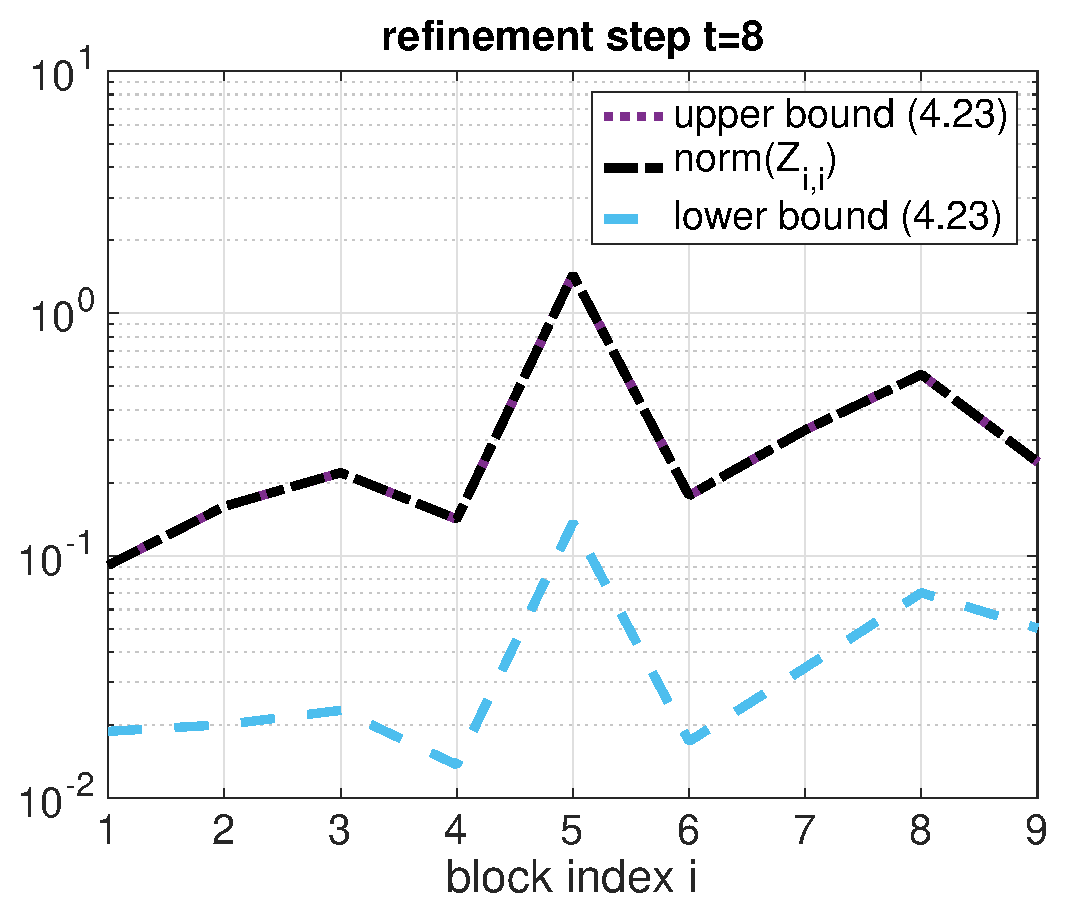
\includegraphics[scale=0.18]{figures/9times9_Z3_Bounds_t8.eps}
% \caption{Relative errors $\E^{\text{u}}_{ij}$ (top row), and upper and lower bounds on $\|\Z_{ii}\|_2$ (bottom row) for the matrix $\A$ of Example~\ref{ex:BDiDo:nonsym2}.}
% \label{fig:BDiDo:ex:nonsym2}
% \end{figure}
%
\vspace*{1em}
\begin{figure}[h!]
\hspace{-1cm}
\centering
\hspace*{2em}
\begin{minipage}[t]{0.48\linewidth}
\centering
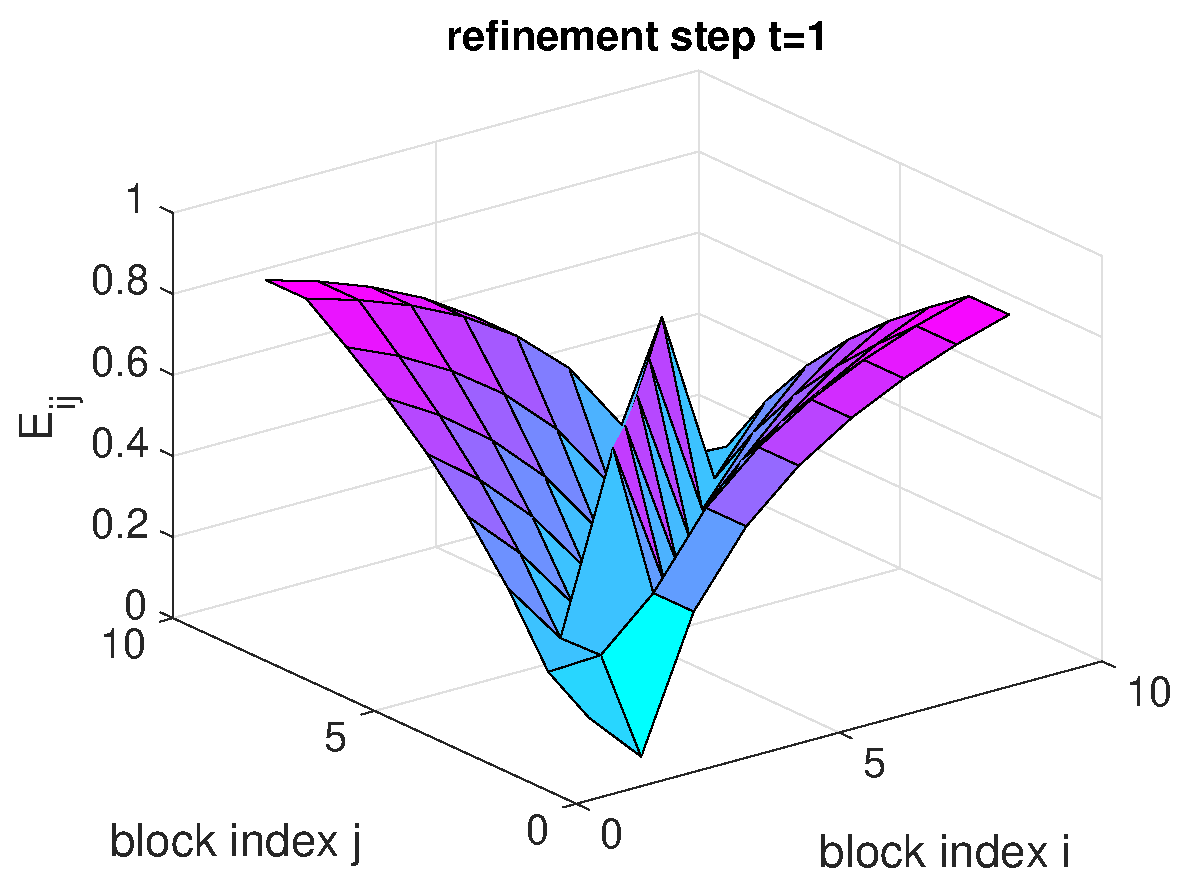
\includegraphics[width=0.99\linewidth]{figures/9times9_Z3_Error_t1.eps}
\end{minipage}
%
\begin{minipage}[t]{0.48\linewidth}
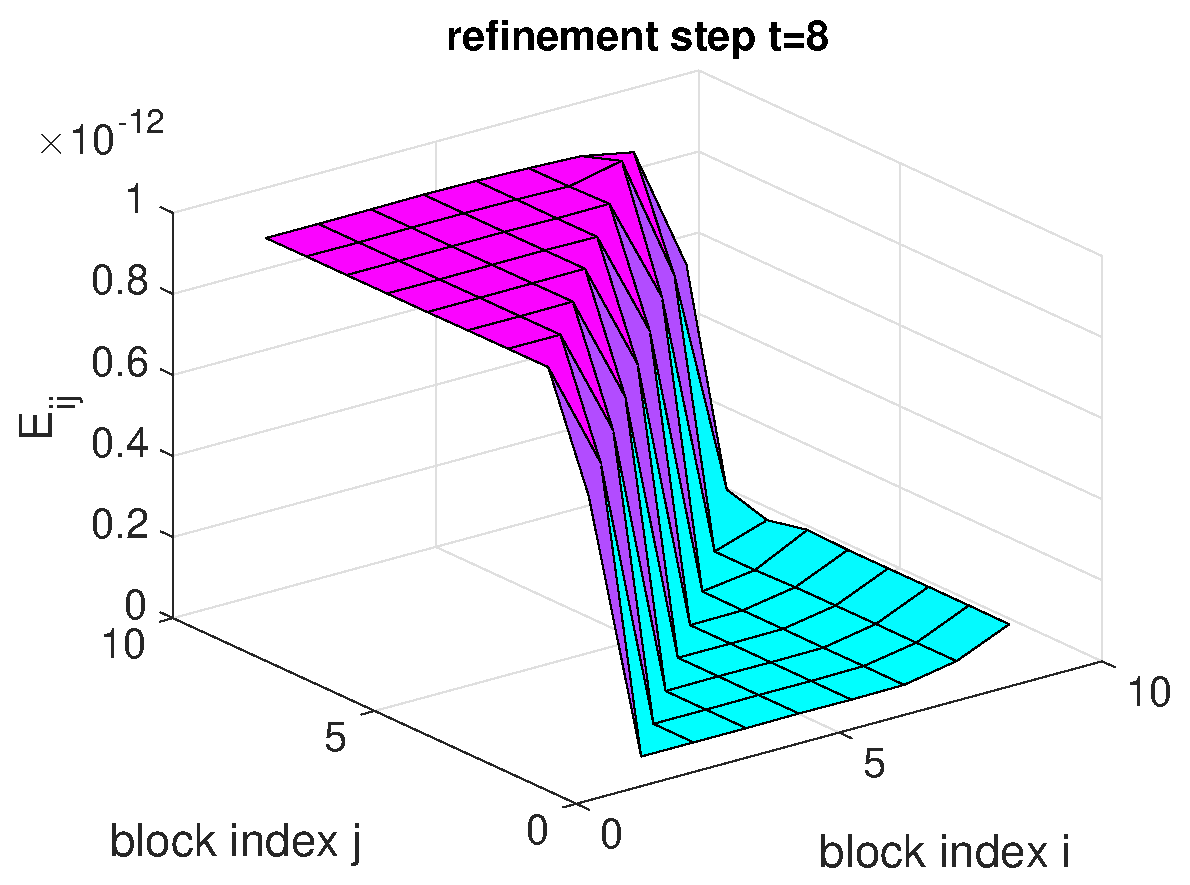
\includegraphics[width=0.99\linewidth]{figures/9times9_Z3_Error_t8.eps}
\end{minipage}
\\\vspace{3em}
\begin{minipage}[t]{0.48\linewidth}
\centering
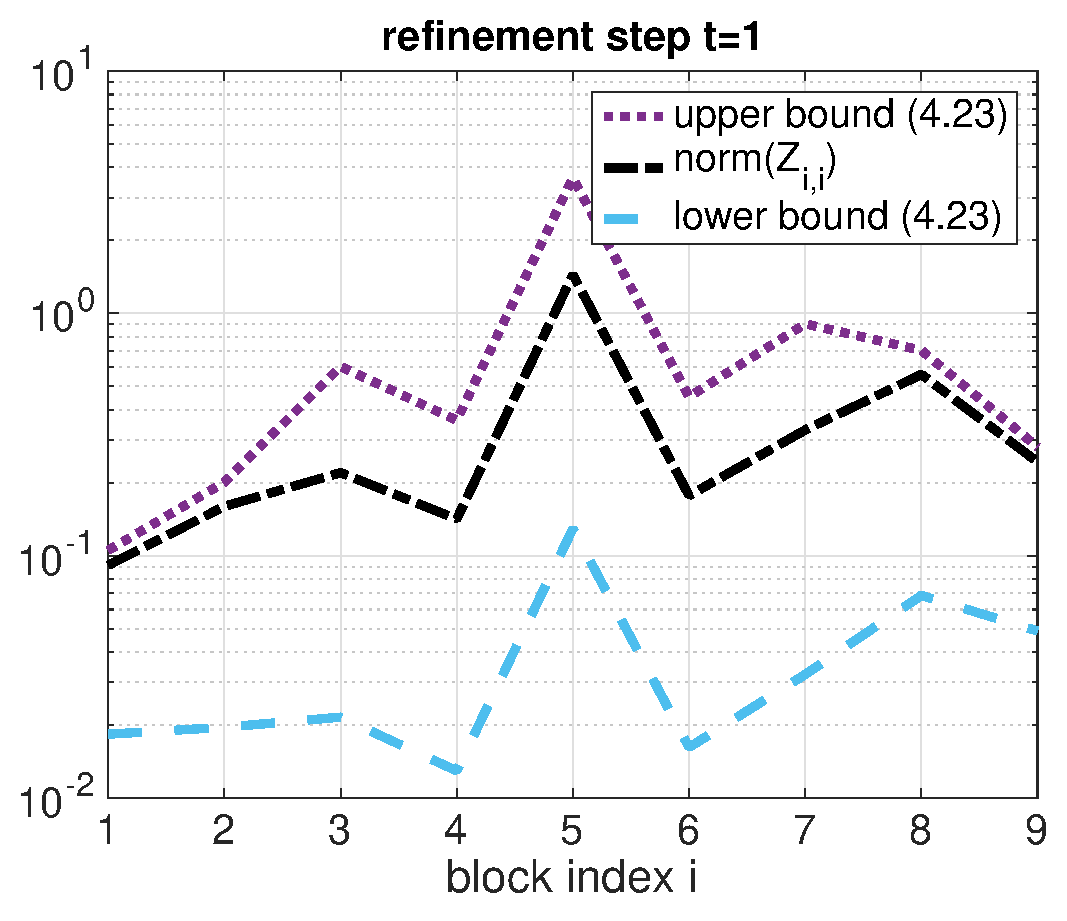
\includegraphics[width=0.99\linewidth]{figures/9times9_Z3_Bounds_t1.eps}
\end{minipage}
%
\begin{minipage}[t]{0.48\linewidth}
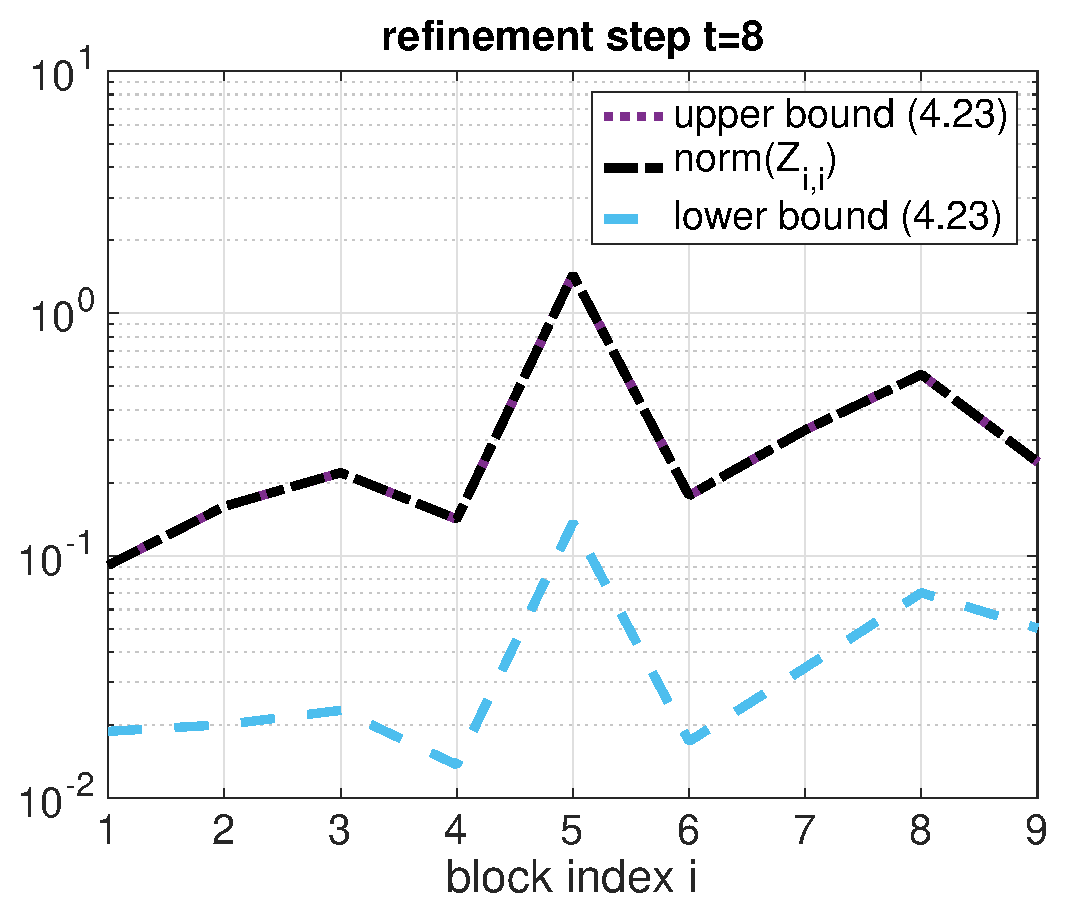
\includegraphics[width=0.99\linewidth]{figures/9times9_Z3_Bounds_t8.eps}
\end{minipage}
\caption{Relative errors $\E^{\text{u}}_{ij}$ (top row), and upper and lower bounds on $\|\Z_{ii}\|_2$ (bottom row) for the matrix $\A$ of Example~\ref{ex:BDiDo:nonsym2}.}
\label{fig:BDiDo:ex:nonsym2}
\end{figure}
}\end{example}

\newpage

\begin{example}\label{ex:BDiDo:nonsym3}{\textrm
Finally, we consider the nonsymmetric block tridiagonal matrix
\begin{equation*}
\A=\\(\R\otimes \I)\tridiag(\tridiag(-0.01,-2,1),\tridiag(-2,10,-2),\tridiag(-0.01,-2,1)),
\end{equation*}
with $\A\in\mathbb{R}^{81\times 81}$, and where $\R\in\mathbb{R}^{9\times 9}$
is a random diagonal matrix constructed as in
\textnormal{Example~\ref{ex:BDiDo:nonsym2}}.
In this case $\A$ takes the form \eqref{eq:BDiDo:blocktridiag} with $\A_i$,
$\B_i$ and $\C_i$ random tridiagonal Toeplitz matrices with integer entries
for all $i$. For this matrix we have $\kappa_2(\A)=58.478$, and
$\|\Z\A-\I\|_2=2.7962\times 10^{-10}$. The relative errors in the bounds
are shown in \textnormal{Figure~\ref{fig:BDiDo:ex:nonsym3}} and the following
table:
%
\begin{table}[h!]\scriptsize\centering
\begin{tabular}{c c c c c c c c c}
\hline
 t & 1 & 2 & 3 & 4 & 5 & 6 & 7 & 8 \\
 $\max_{ij}\E^{u}_{ij}$ &  $0.84477$ & $0.63381$ & $0.39537$ & $0.20898$ & $0.09595$ & $0.03780$ &  $0.01109$ & $7.142\times 10^{-13}$\\
 $\max_{i}\E^{l}_{i}$ &  $0.91039$ & $0.90877$ & $0.90765$ & $0.90529$ & $0.90529$ & $0.90529$ &  $0.90529$ & $0.90529$\\
  \hline
\end{tabular}
%\caption{Values of the maximum relative errors for the matrix $A$ of Example 2.4 and  different values of $t$.}
%\label{tab:errorA4}
\end{table}
%
%\newpage
% \begin{figure}[h!]
% \centering
% 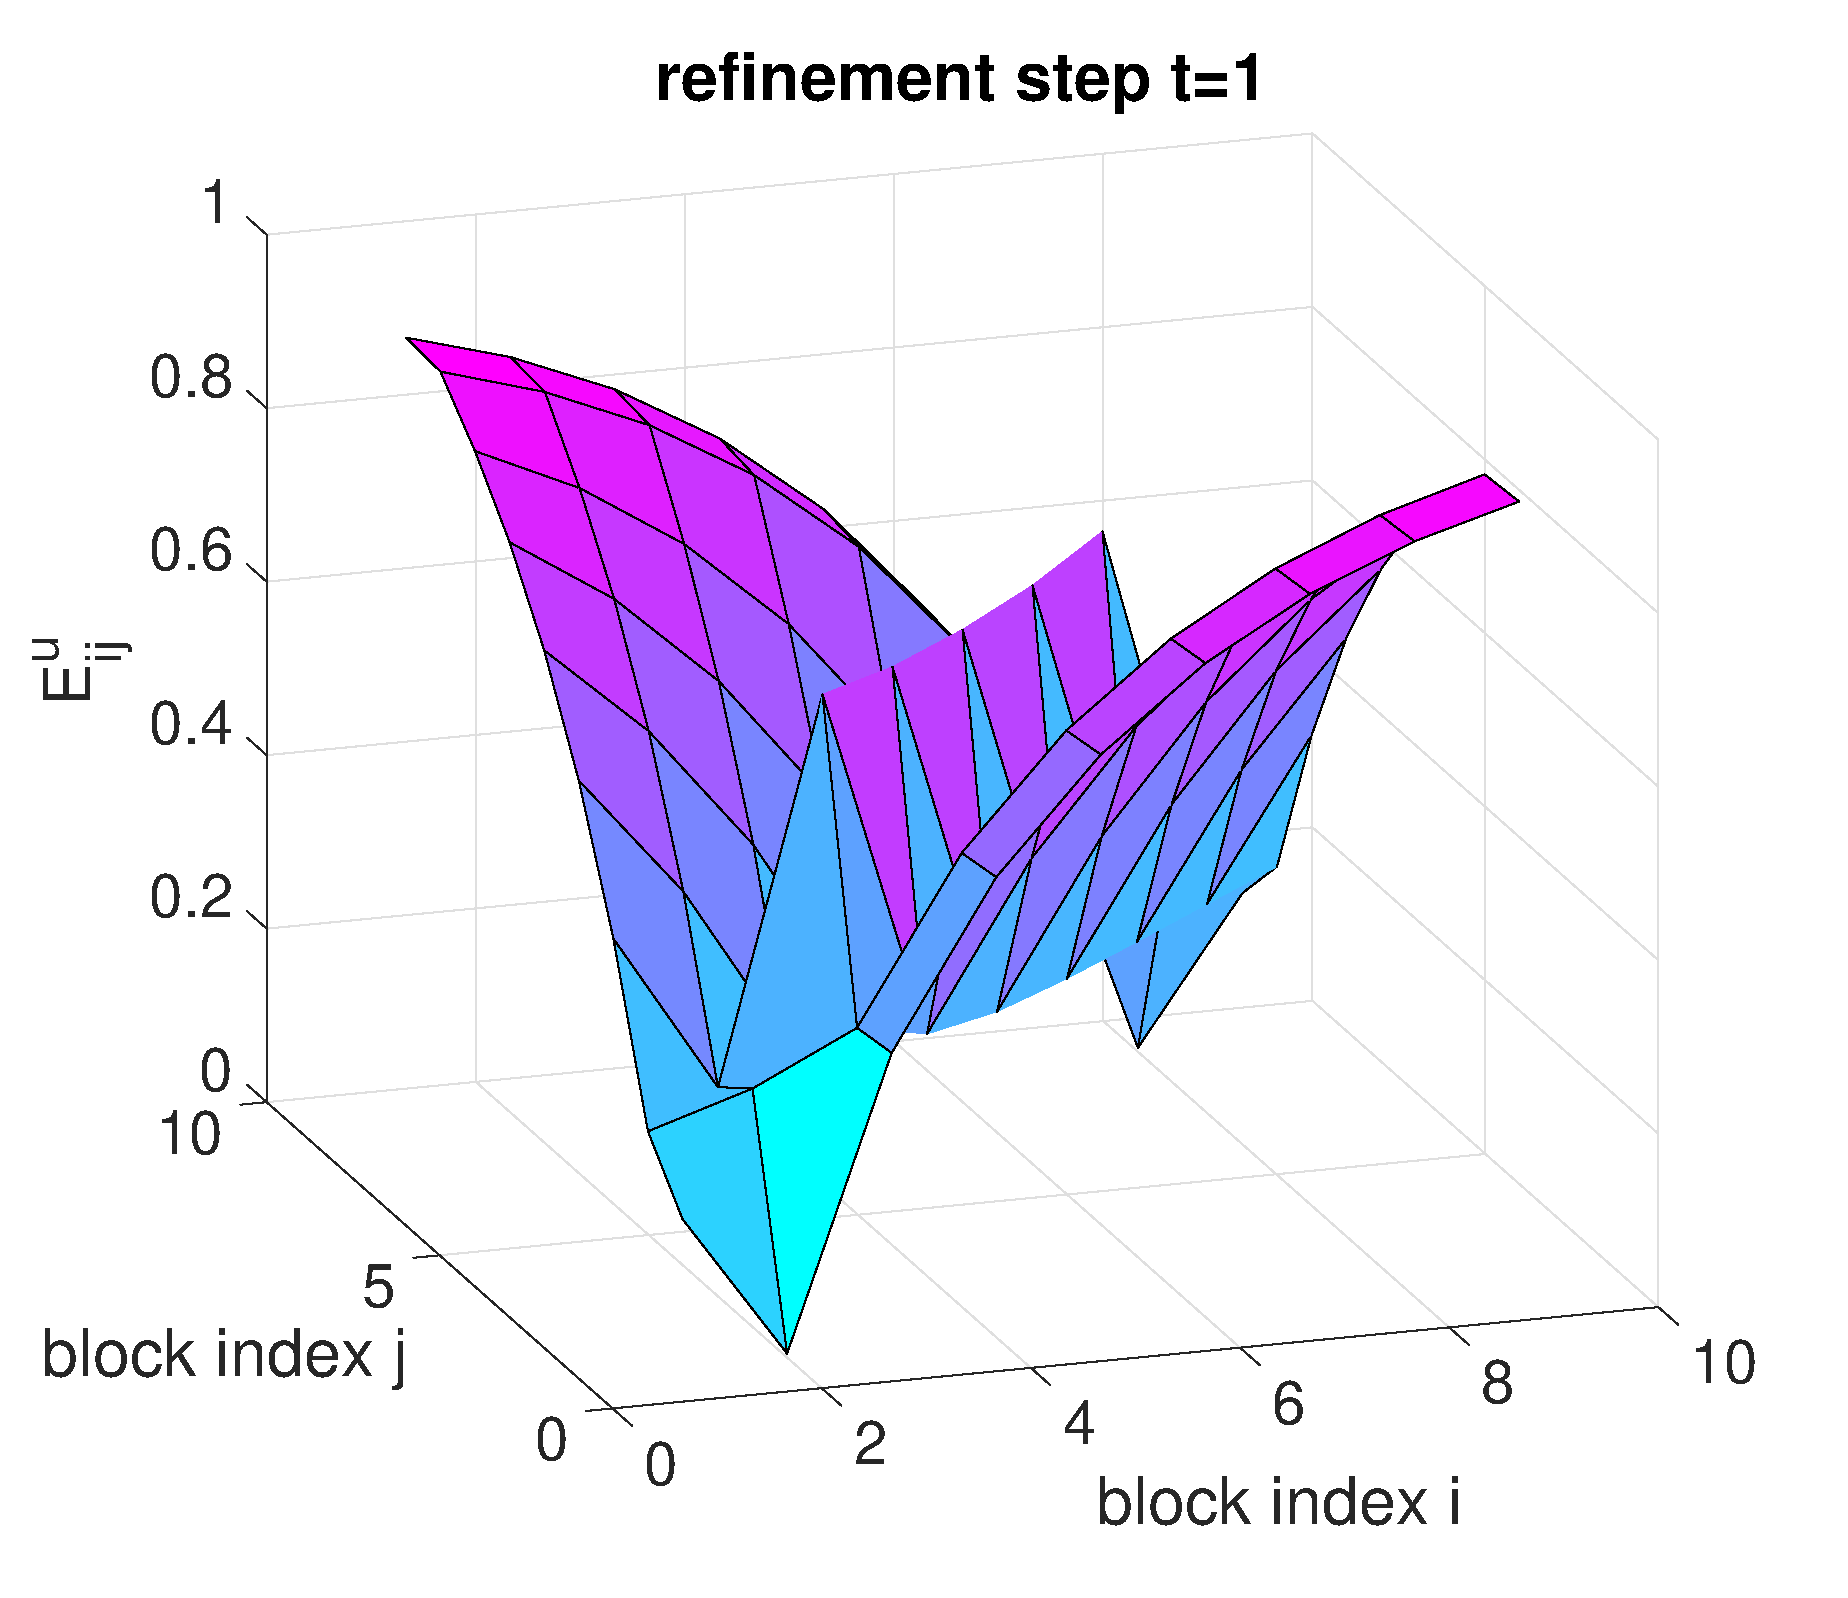
\includegraphics[width=0.475\linewidth]{figures/9times9_Z4_Error_t1b.eps}
% 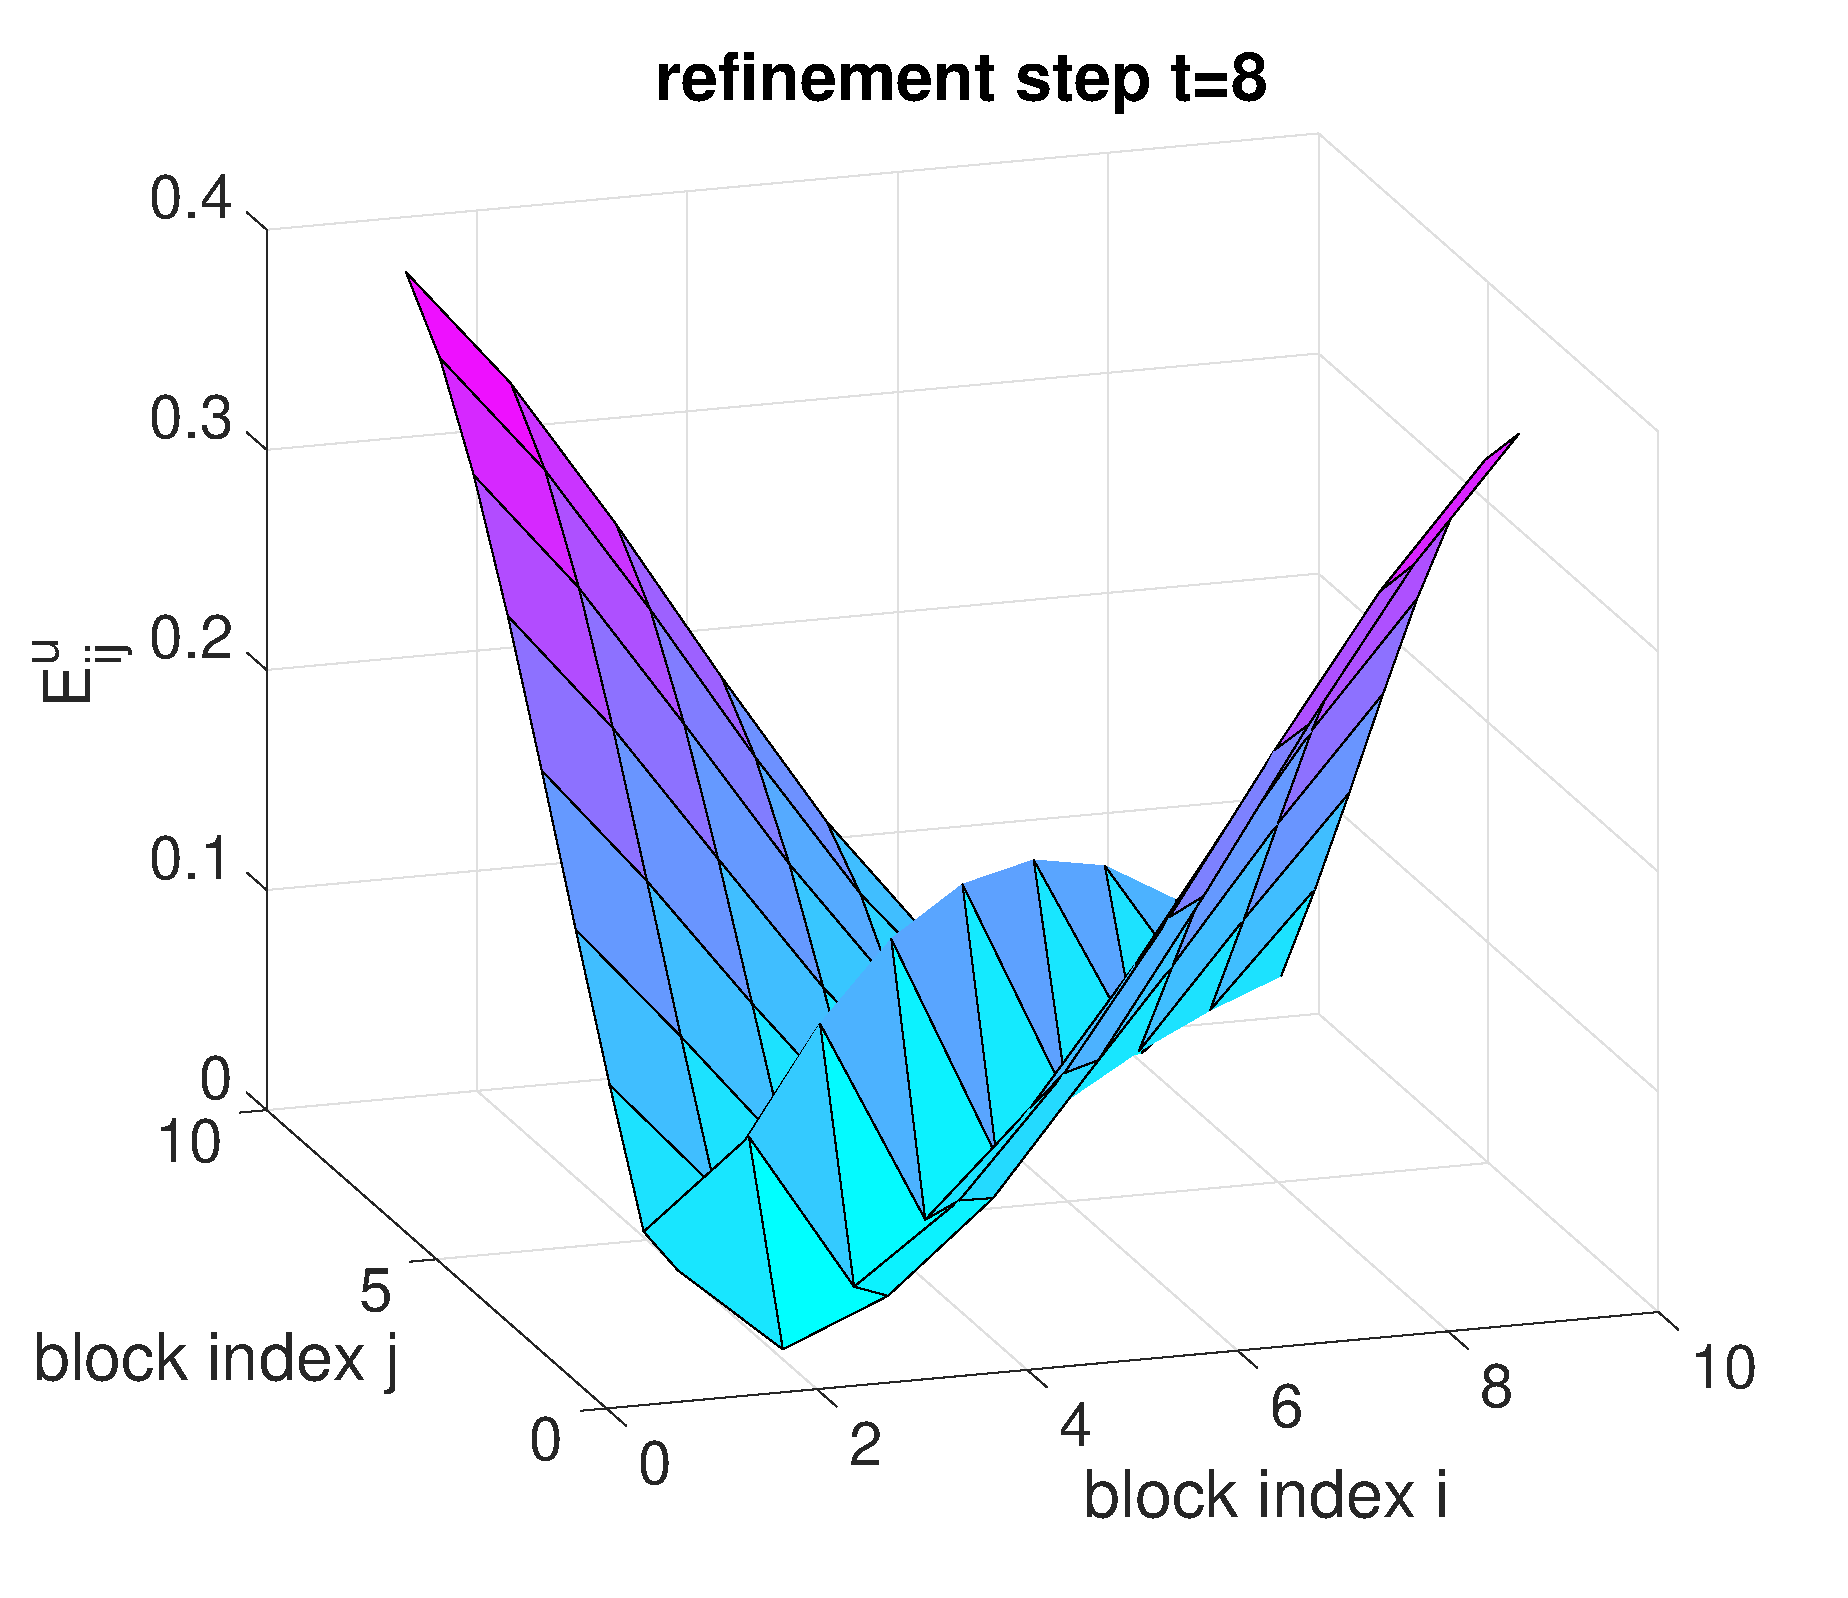
\includegraphics[width=0.475\linewidth]{figures/9times9_Z4_Error_t8b.eps}\\[1ex]
% 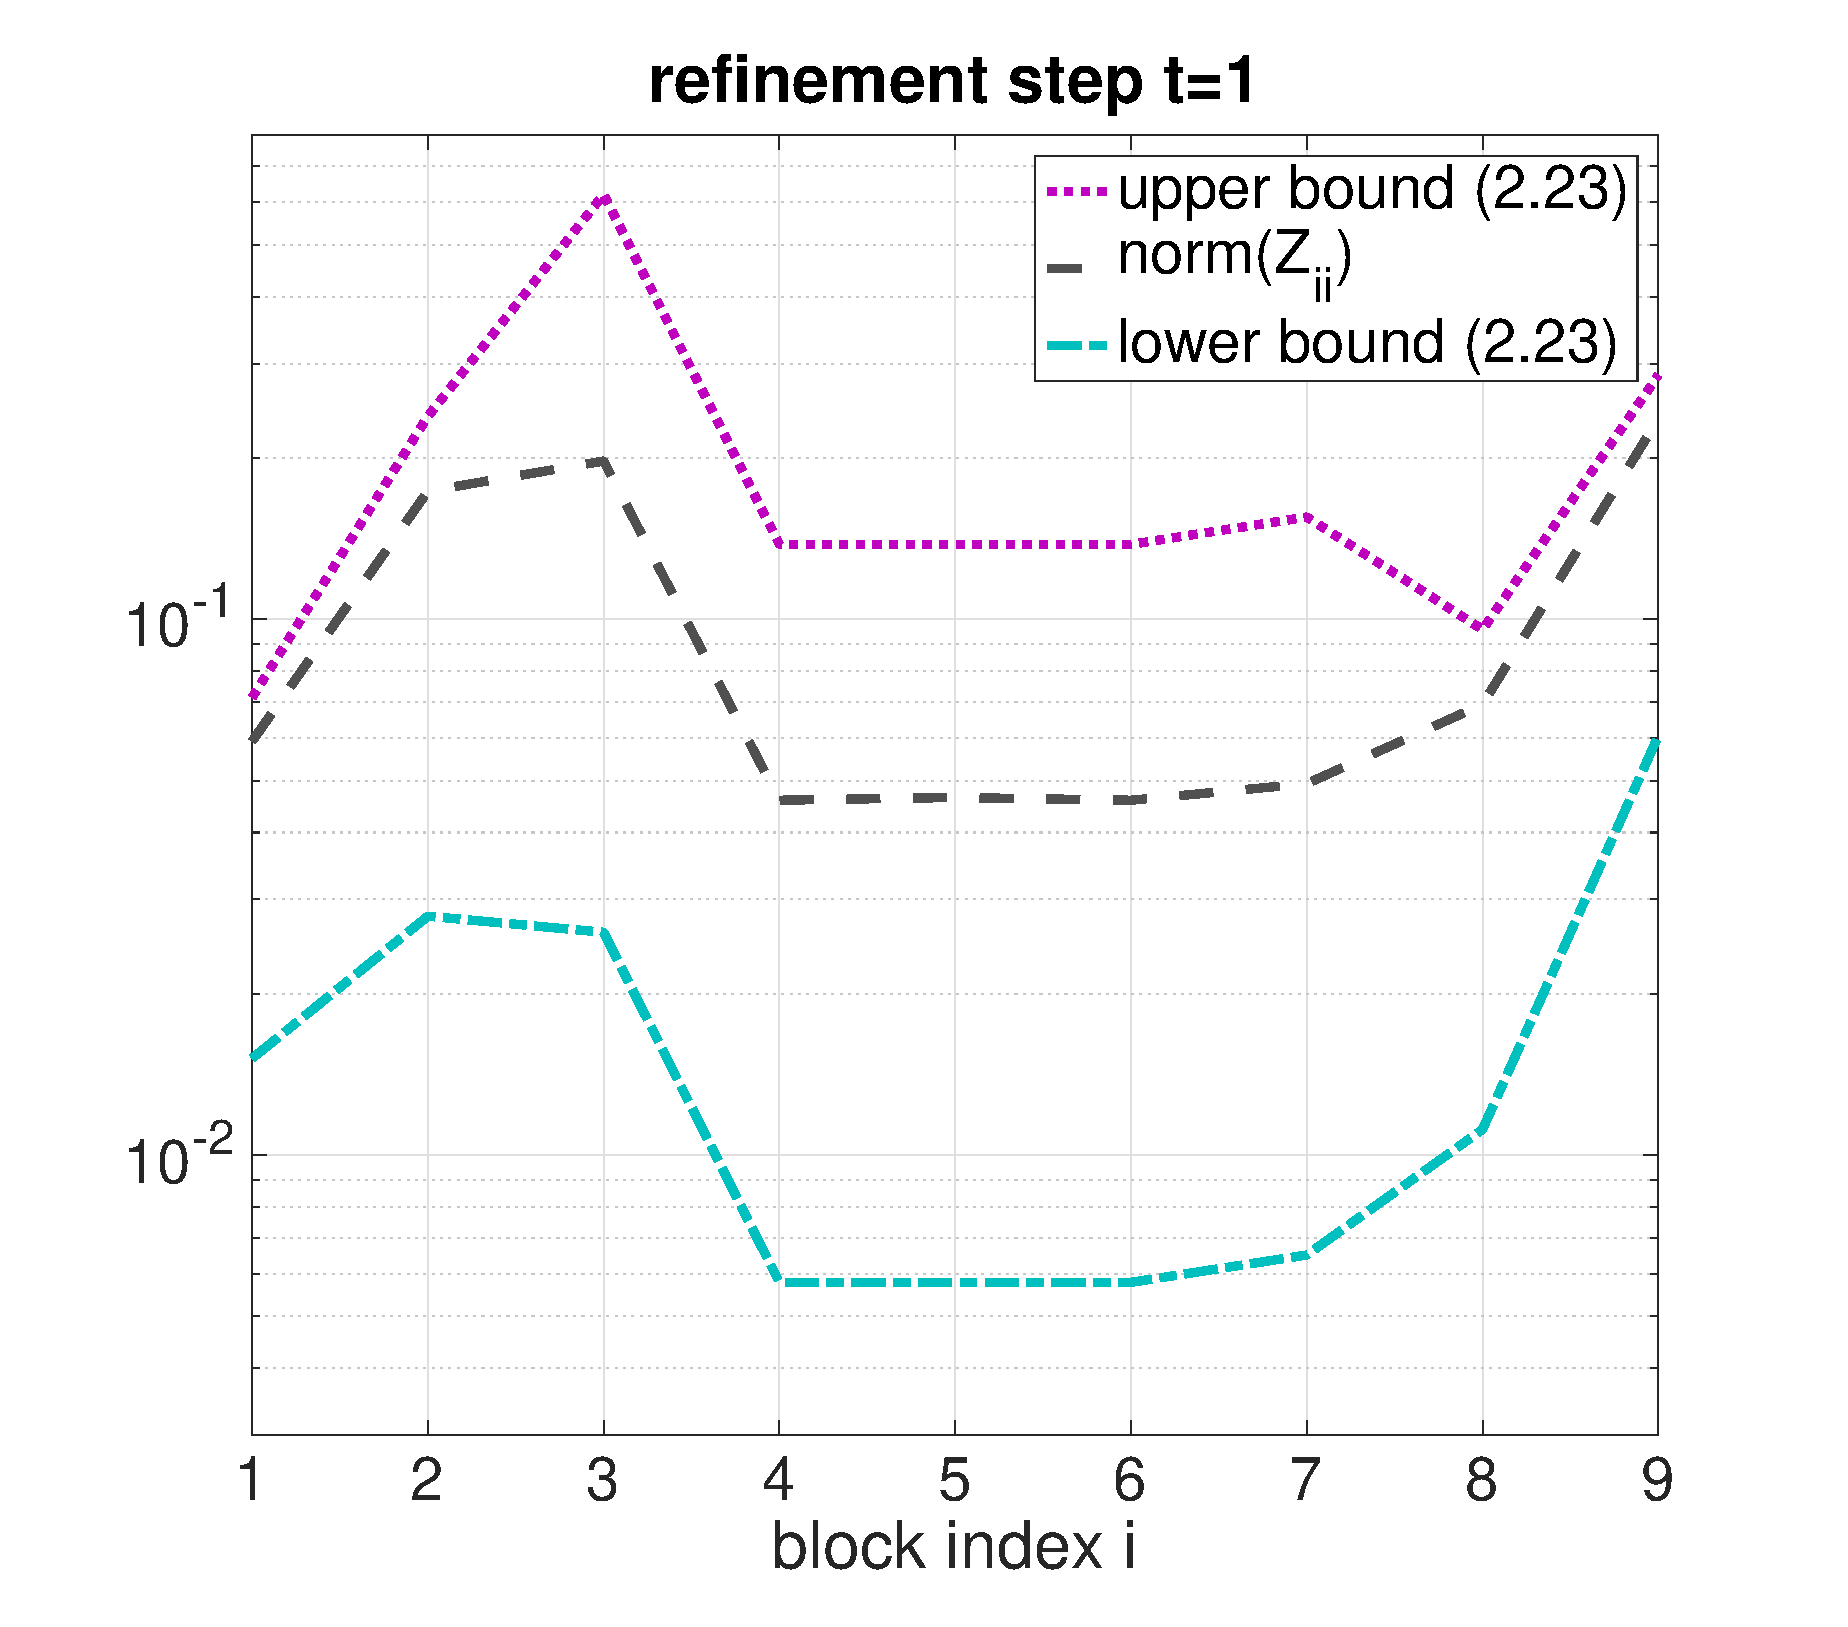
\includegraphics[width=0.475\linewidth]{figures/9times9_Z4_Bounds_t1b.eps}
% 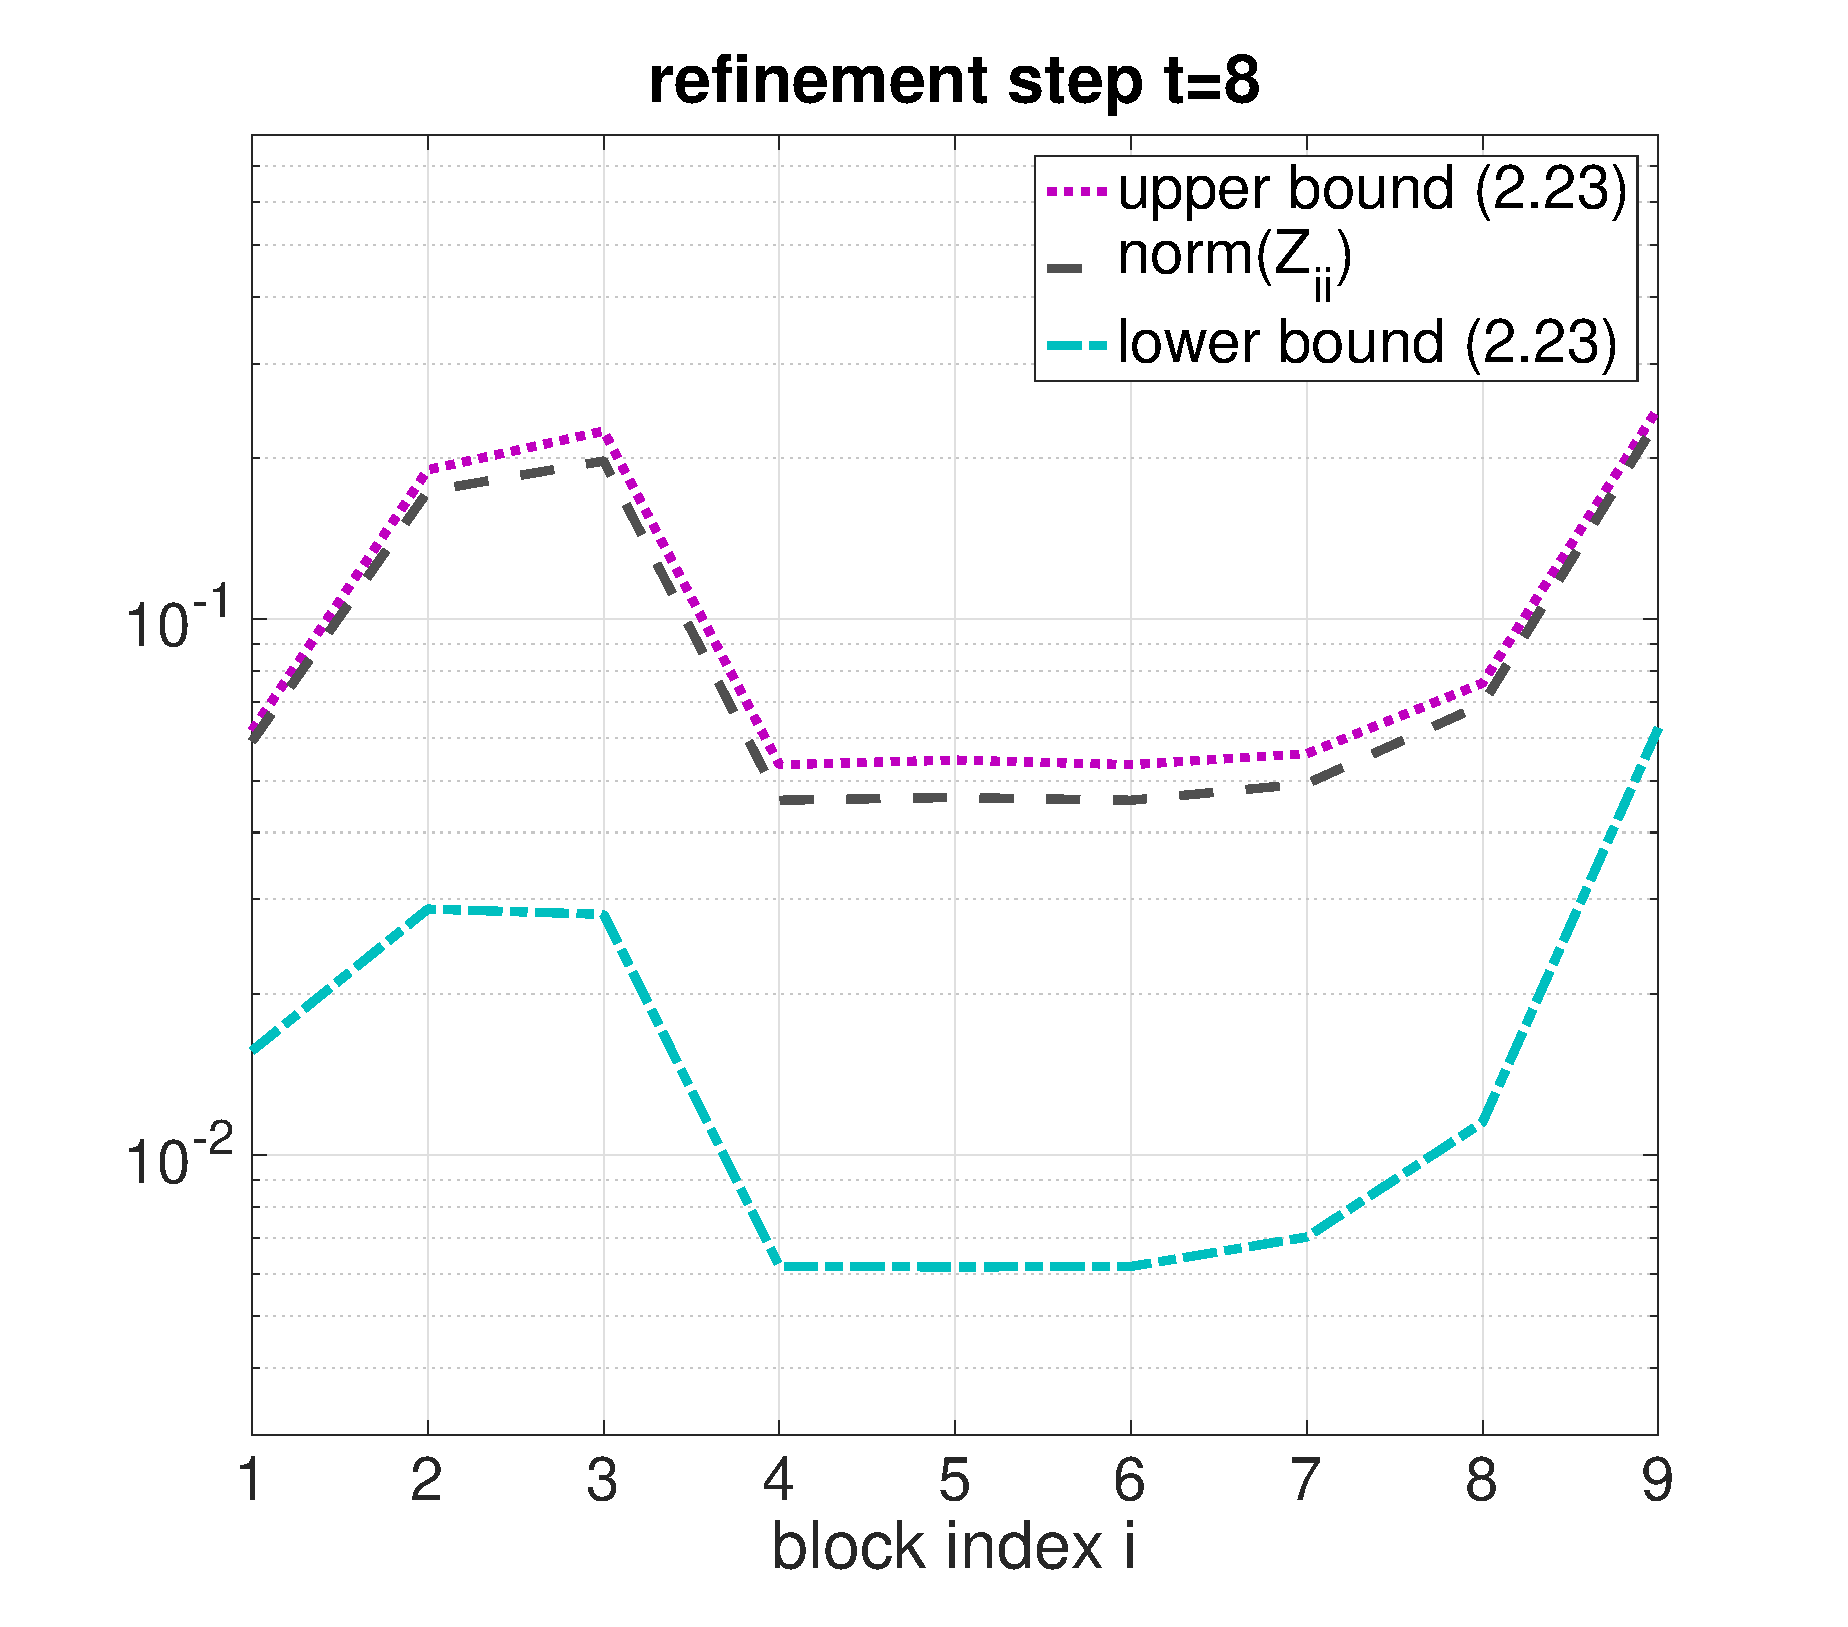
\includegraphics[width=0.475\linewidth]{figures/9times9_Z4_Bounds_t8b.eps}
% \caption{Relative errors $\E^{\text{u}}_{ij}$ (top row), and upper and lower bounds on $\|\Z_{ii}\|_2$ (bottom row) for the matrix $\A$ of Example~\ref{ex:BDiDo:nonsym3}.}
% \label{fig:BDiDo:ex:nonsym3}
% \end{figure}
\vspace*{2em}
\begin{figure}[h!]
%\vspace{-1.1em}
\hspace{-1cm}
\centering
\hspace*{2em}
\begin{minipage}[t]{0.48\linewidth}
\centering
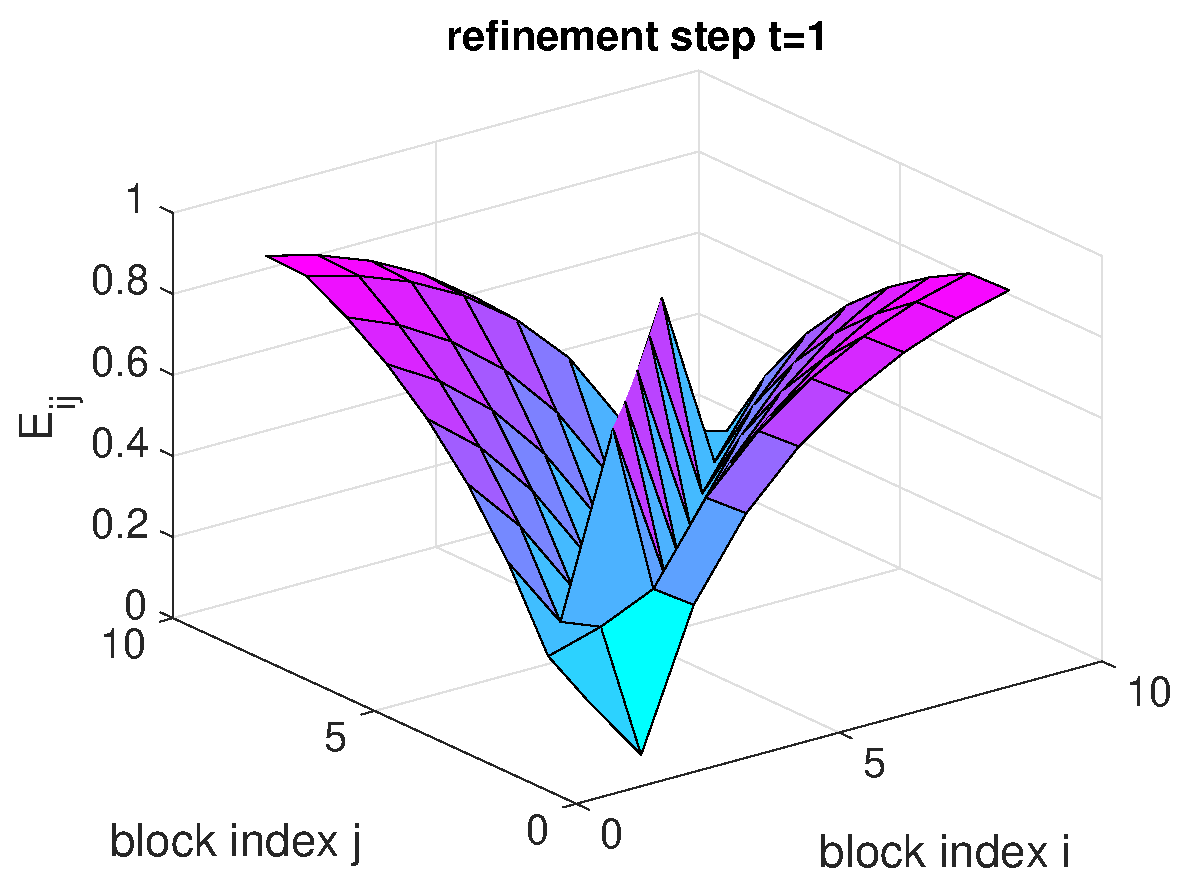
\includegraphics[width=0.99\linewidth]{figures/9times9_Z4_Error_t1.eps}
\end{minipage}
%
\begin{minipage}[t]{0.48\linewidth}
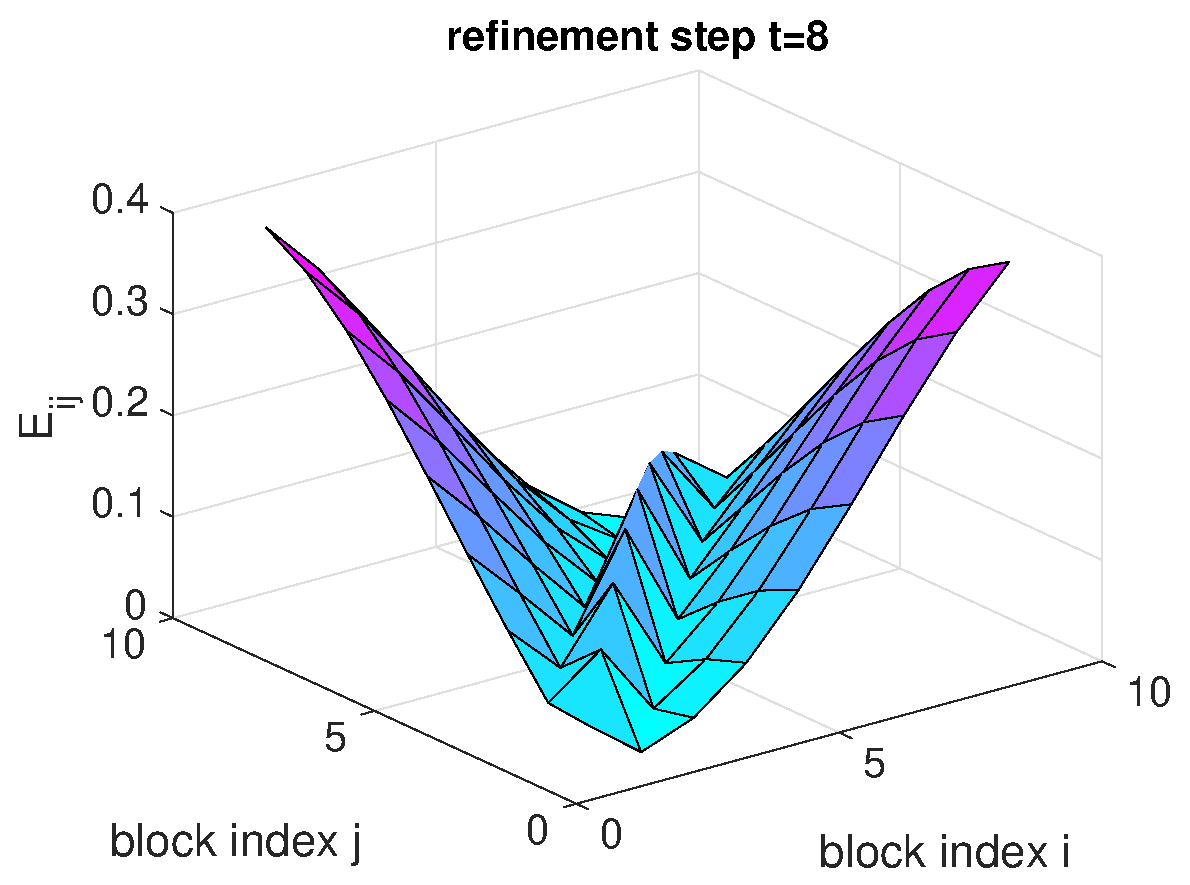
\includegraphics[width=0.99\linewidth]{figures/9times9_Z4_Error_t8.eps}
\end{minipage}
\\\vspace{4em}
\begin{minipage}[t]{0.48\linewidth}
\centering
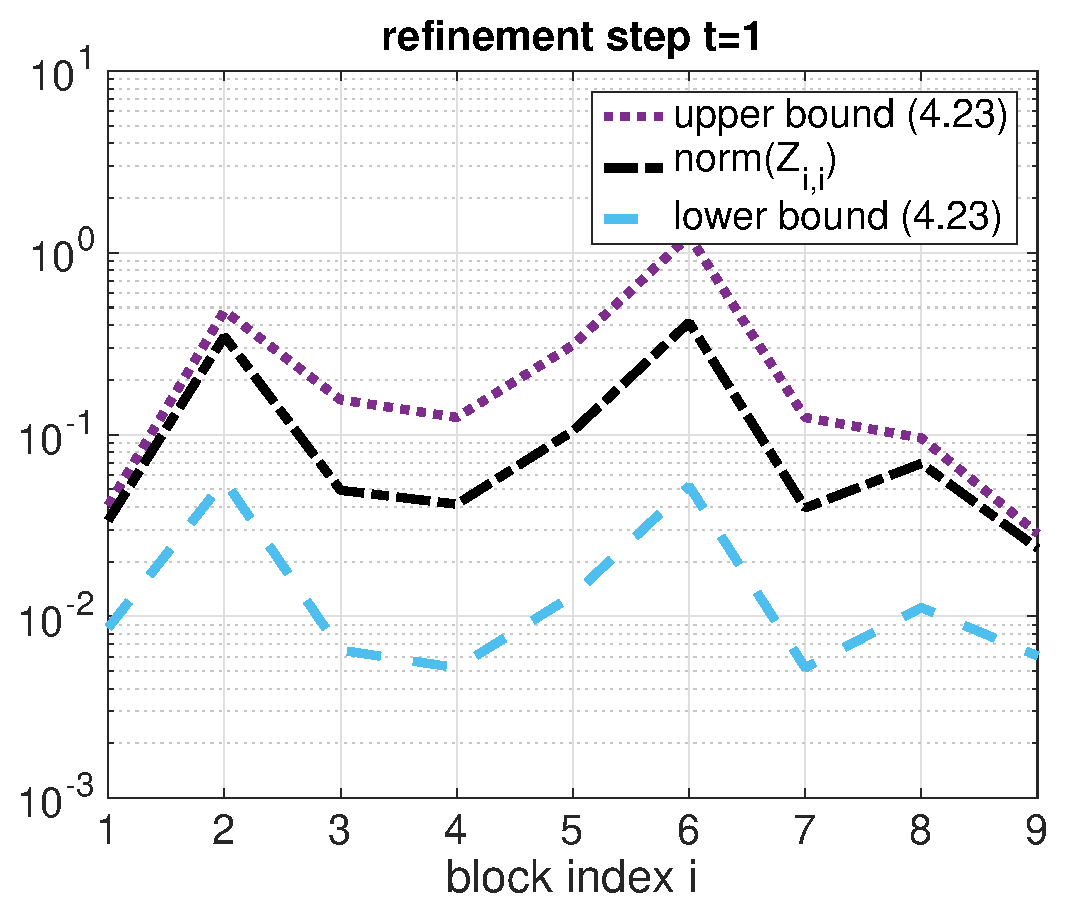
\includegraphics[width=0.99\linewidth]{figures/9times9_Z4_Bounds_t1.eps}
\end{minipage}
%
\begin{minipage}[t]{0.48\linewidth}
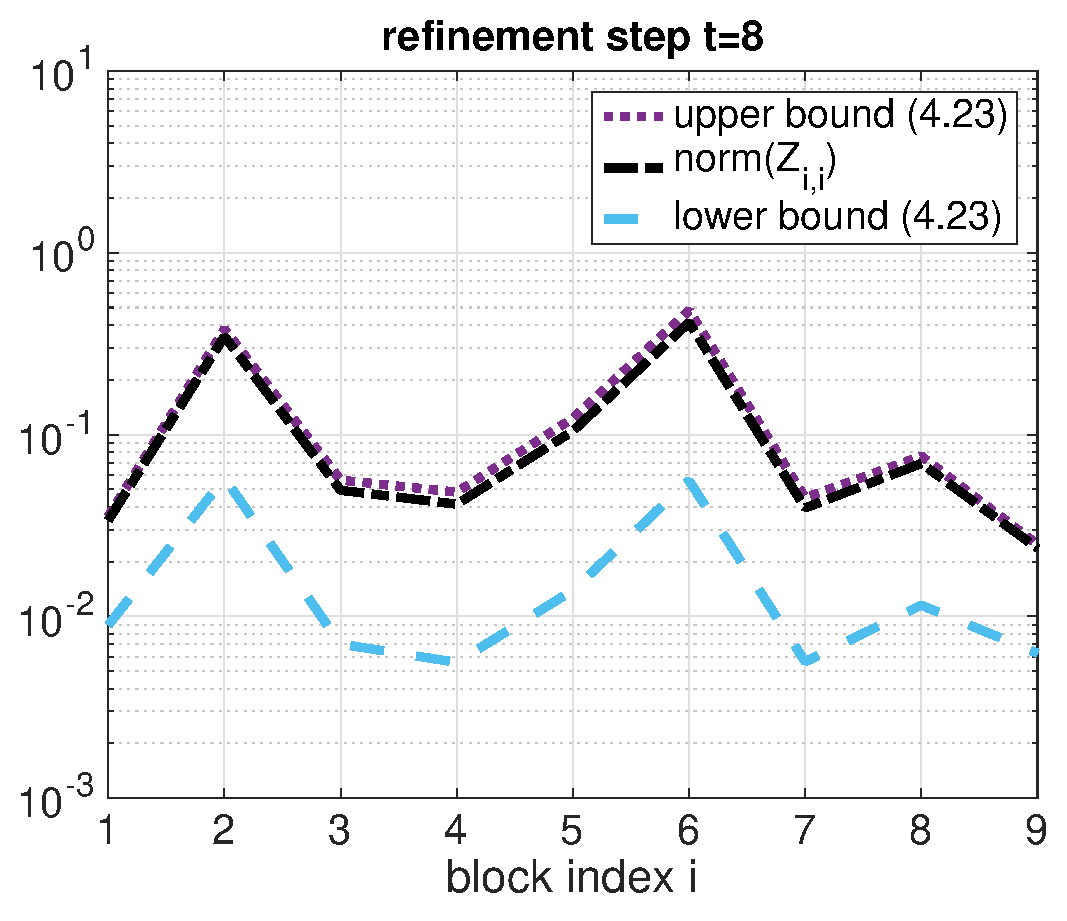
\includegraphics[width=0.99\linewidth]{figures/9times9_Z4_Bounds_t8.eps}
\end{minipage}
\caption{Relative errors $\E^{\text{u}}_{ij}$ (top row), and upper and lower bounds on $\|\Z_{ii}\|_2$ (bottom row) for the matrix $\A$ of Example~\ref{ex:BDiDo:nonsym3}.}
\label{fig:BDiDo:ex:nonsym3}
\end{figure}
}\end{example}

\newpage

% \subsection{Eigenvalue Inclusion Sets}
% \label{BDiDo:numerics:sets}
% %
We continue by providing a set of numerical illustrations of of the newly
proposed eigenvalue inclusion sets, $G_i^{\text{new}}$, which are a consequence
of Corollary~\ref{cor:BDiDo:inclusion}. We consider different matrices
$\A=[\A_{ij}]$, and we compute the boundaries of the sets $G_i^{\text{new}}$ and
$G_i^{\text{FV}}$ for all $i\leq n$, i.e., the curves for $z\in {\mathbb C}$
where
\begin{equation*}
\sum_{\atopfrac{j=1}{j\neq i}}^{n}\| (\A_{ii}-z \I)^{-1} \A_{ij} \|=1,\text{ and }
%\quad i,j\in\{1,2\},\quad i\neq j,\\
\sum_{\atopfrac{j=1}{j\neq i}}^{n}\| (\A_{ii}-z \I)^{-1}\|\| \A_{ij} \|=1,
\quad i,j\in\{1,\ldots,n\},\quad i\neq j,
\end{equation*}
%
respectively.

\begin{example}\label{ex:BDiDo:inclusion}{\textrm
We first consider the symmetric matrix
\begin{equation}\label{eq:BDiDo:ELNmatrix1}
\A=
\left[ \begin{array}{rr|rr}
4	& -2	& -1 & 1	\\
-2	&	4	&  0 & -1	\\ \hline
-1	& 0	&	4	&-2	\\
1	& -1	& -2	& 4
\end{array} \right]
=
\left[ \begin{array}{c|c}
\A_{11}	& \A_{12}	\\ \hline
\A_{21}	& \A_{22}
\end{array} \right],
\end{equation}
which has the eigenvalues $1.4586$, $2.3820$, $4.6180$, and $7.5414$
(computed in \textnormal{\texttt{MATLAB}} and rounded to five significant
digits). \textnormal{Figure~\ref{fig:BDiDo:ex:inclusion1}}
shows the boundaries of the corresponding sets $G_i^{\text{new}}$ and
$G_i^{\text{FV}}$ for $i=1,2$, i.e., the curves for $z\in {\mathbb C}$ where
%
%\begin{eqnarray*}
%&& \| (A_{ii}-z I)^{-1} A_{ij} \|=1,\quad \| A_{ij} (A_{ii}-z I)^{-1}  \|=1,
%\quad i,j\in\{1,2\},\quad i\neq j,\\
%&&\| (A_{ii}-z I)^{-1}\|\| A_{ij} \|=1,
%\quad i,j\in\{1,2\},\quad i\neq j,
%\end{eqnarray*}
%
\begin{equation*}
\| (\A_{ii}-z \I)^{-1} \A_{ij} \|=1,\text{ and }
%\quad i,j\in\{1,2\},\quad i\neq j,\\
\| (\A_{ii}-z \I)^{-1}\|\| \A_{ij} \|=1,
\quad i,j\in\{1,2\},\quad i\neq j,
\end{equation*}
%
respectively. Clearly, the sets $G_i^{\text{new}}$ give tighter inclusion
regions for the eigenvalues than the sets $G_i^{\text{FV}}$ as well as the
usual Gershgorin circles for the matrix $\A$, which are given by the two
circles centered at $z=4$ of radius~3 and~4.

\begin{figure}[h!]
\centering
\vspace*{-0.4cm}
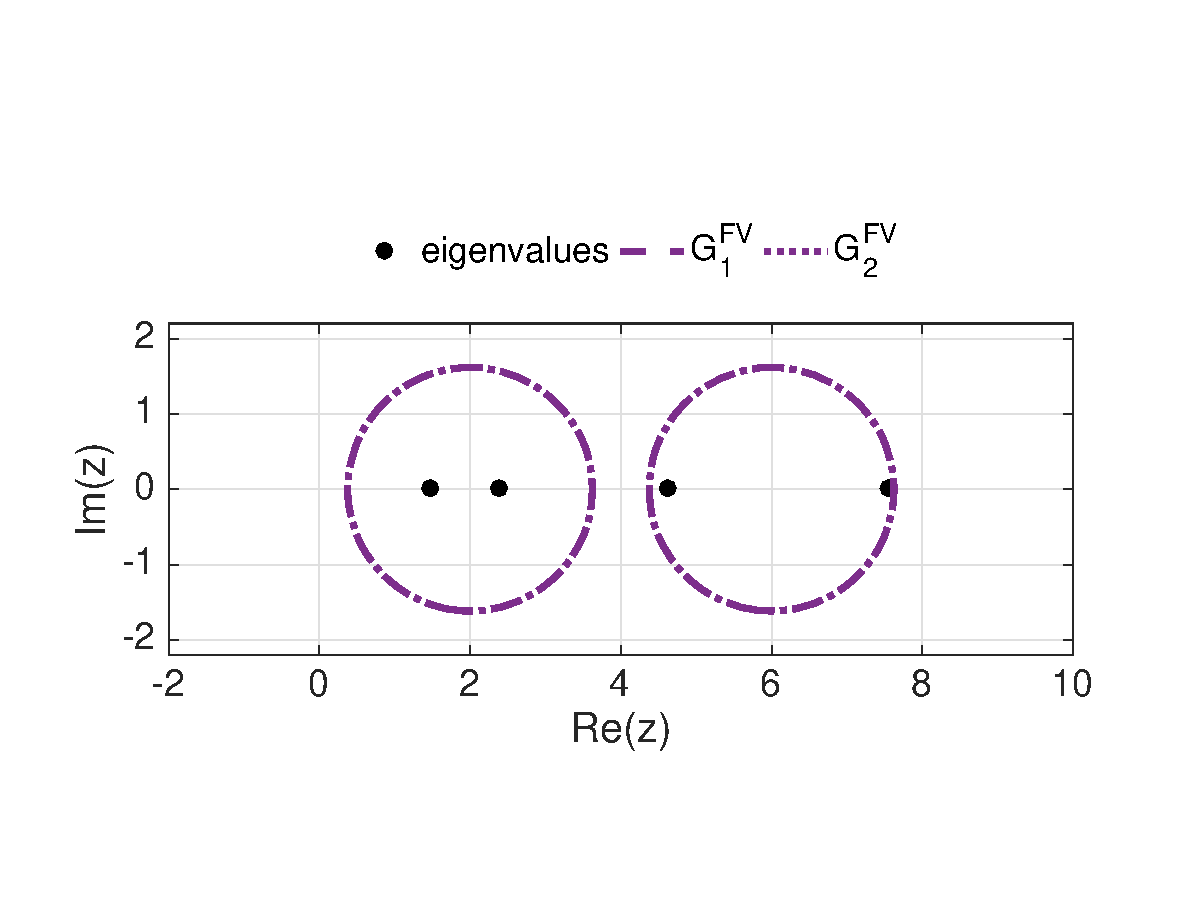
\includegraphics[width=0.49\linewidth]{figures/Example415_a1}
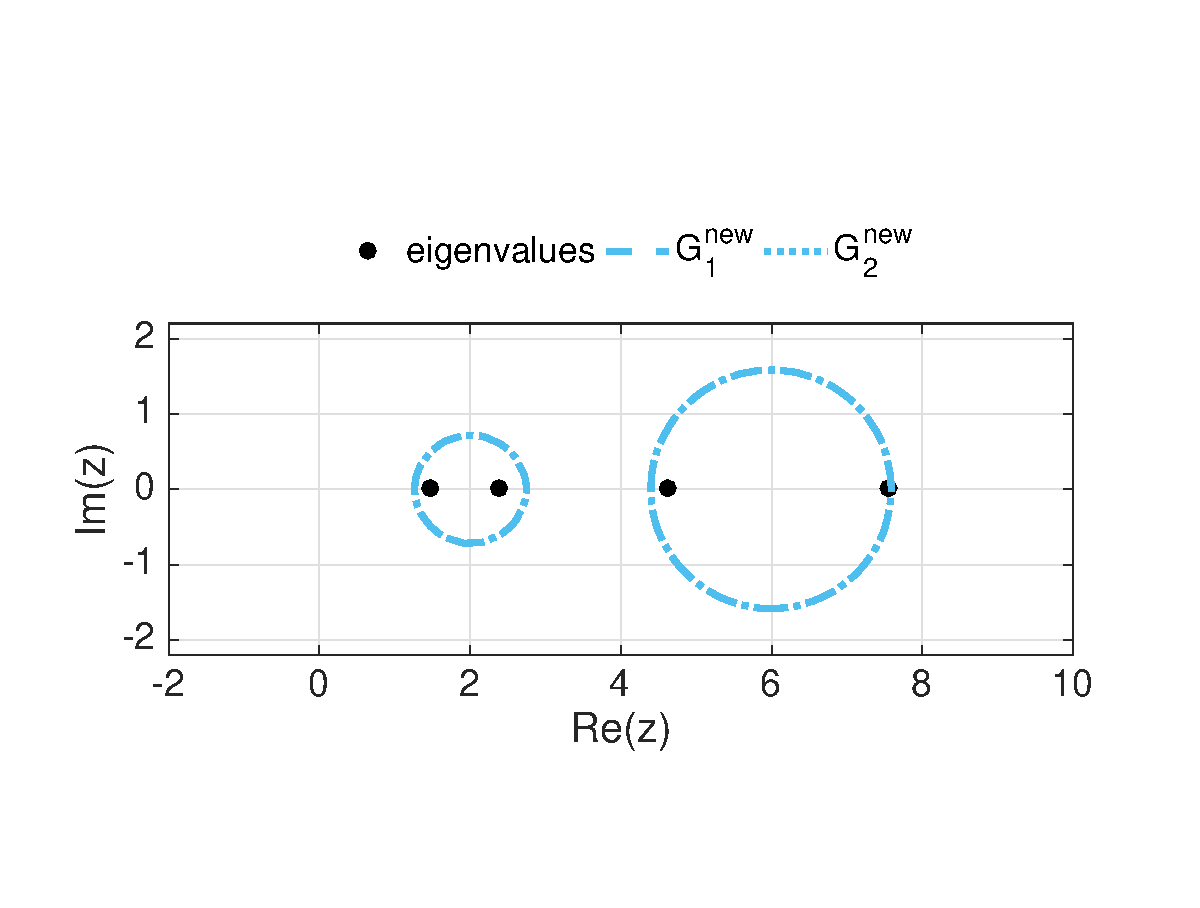
\includegraphics[width=0.49\linewidth]{figures/Example415_a2}
\vspace*{-0.5cm}
\caption{Eigenvalue inclusion regions obtained from the sets
$G_i^{\text{new}}$ and $G_i^{\text{FV}}$ for the matrix \eqref{eq:BDiDo:ELNmatrix1} of Example~\ref{ex:BDiDo:inclusion}.}
\label{fig:BDiDo:ex:inclusion1}
\end{figure}

We next consider the nonsymmetric matrix
\begin{equation}\label{eq:BDiDo:ELNmatrix2}
\A=
\left[ \begin{array}{rr|rr}
4	& -2	& -0.5 & 0.5	\\
-2	&	5	&  -1.4 & -0.5	\\ \hline
-0.5	& 0	&	4	&-2	\\
0.5	& -0.5	& -2	& 4
\end{array} \right]
=
\left[ \begin{array}{c|c}
\A_{11}	& \A_{12}	\\ \hline
\A_{21}	& \A_{22}
\end{array} \right],
\end{equation}
which has the eigenvalues $1.6851$, $2.5959$, $6.2263$, and $6.4927$. As shown
in \textnormal{Figure~\ref{fig:BDiDo:ex:inclusion2}}, the sets
$G_i^{\text{new}}$ again give tighter inclusion regions than the sets
$G_i^{\text{FV}}$ as well as the usual Gershgorin circles.
%
\begin{figure}[tbph]
\centering
\vspace*{-0.4cm}
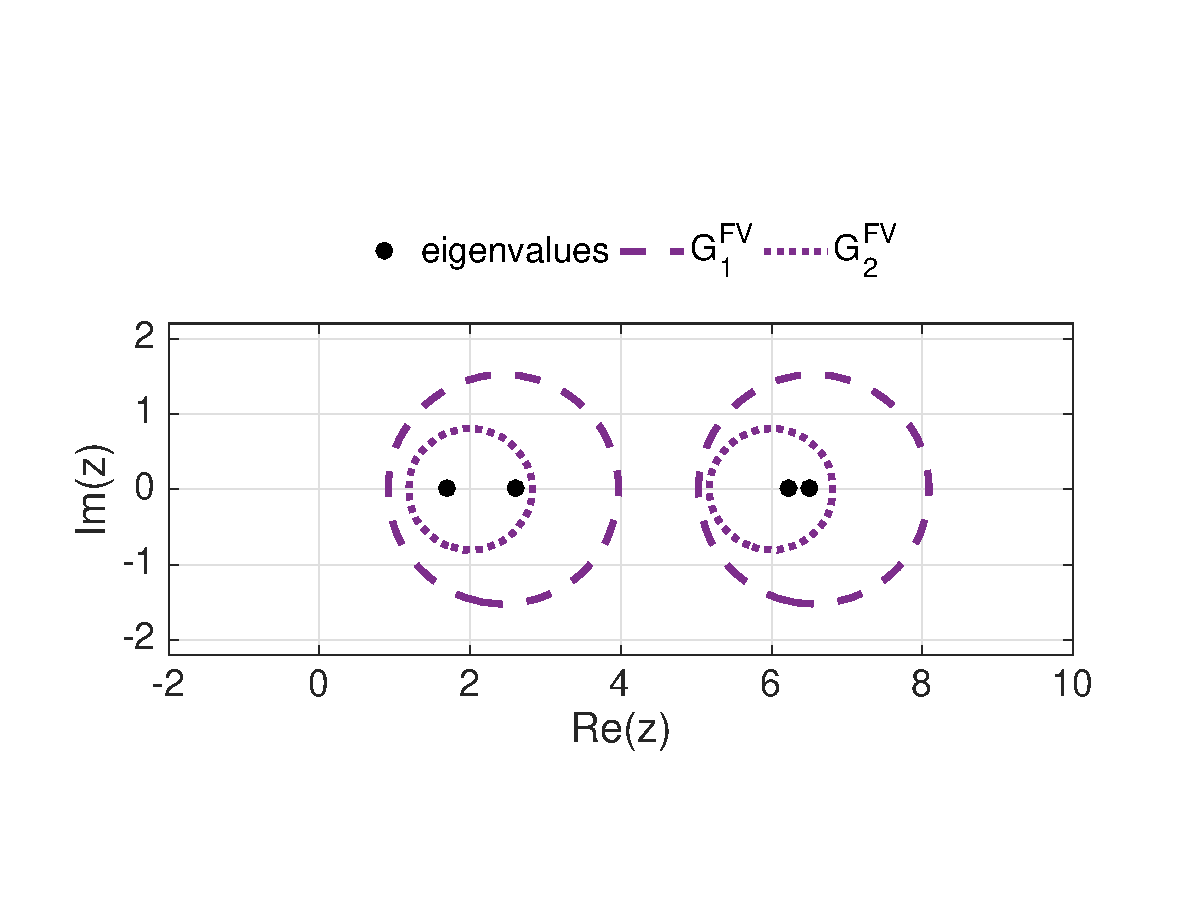
\includegraphics[width=0.49\linewidth]{figures/Example415_b1}
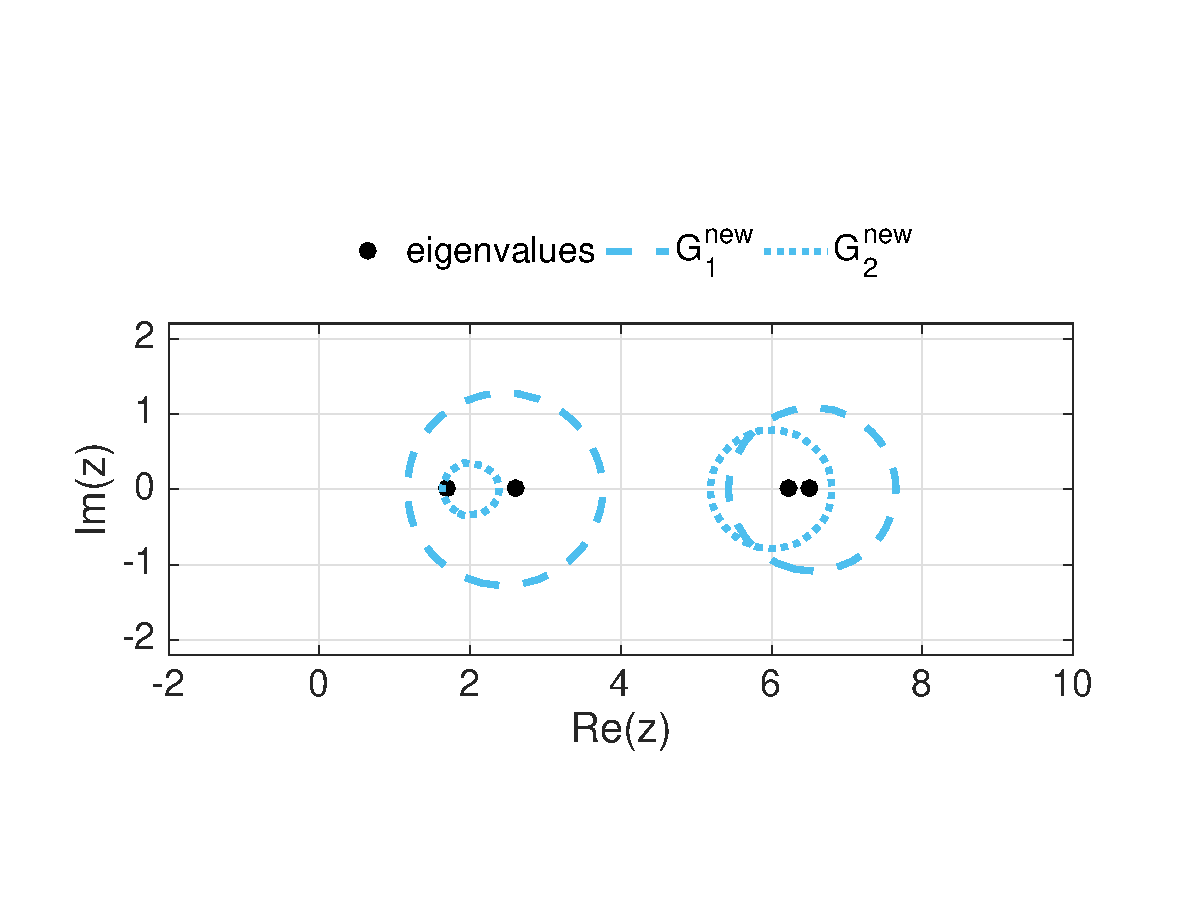
\includegraphics[width=0.49\linewidth]{figures/Example415_b2}
\vspace*{-0.5cm}
\caption{Eigenvalue inclusion regions obtained from the sets
$G_i^{\text{new}}$ and $G_i^{\text{FV}}$ for the matrix \eqref{eq:BDiDo:ELNmatrix2} of Example~\ref{ex:BDiDo:inclusion}.}
\label{fig:BDiDo:ex:inclusion2}
\end{figure}
}\end{example}

% In the next example, we show the inclusion sets for larger matrices.

% \begin{example}\label{ex:BDiDo:inclusion2}{\textrm
% Consider the symmetric block tridiagonal matrix $\A$ given by
% \[
% \A~=\I_9\otimes~\T_1+\T_2\otimes \I_5 \;\;\in\;\;\mathbb{R}^{45\times 45},
% \]
% where $\T_1=\textnormal{tridiag}(-2,2,-2) \in {\mathbb R}^{9\times 9}$ and
% $\T_2=\textnormal{tridiag}(-0.5,2,-0.5)\in {\mathbb R}^{5\times 5}$.
% Thus, $\A$ is of the form \eqref{eq:BDiDo:blocktridiag} with constant
% tridiagonal Toeplitz matrices $\A_i=\textnormal{tridiag}(-2,4,-2)\in {\mathbb R}^{9\times 9}$ and constant diagonal matrices $\B_i=\C_i=\textnormal{diag}(-0.5)\in {\mathbb R}^{9\times 9}$ for all $i$; its structure is
% shown in the left part of \textnormal{Figure~\ref{fig:BDiDo:ex:inclusion2_b}}.
% % and has the eigenvalues\td{\textbf{add:}eigenvalues of this matrix.}
% %(computed in \texttt{MATLAB} and rounded to five significant digits).
% %
%
% The boundaries of the corresponding sets $G_i^{\text{new}}$ and $G_i^{FV}$ for
% $i=1,\ldots,9$ are shown on the left side of
% \textnormal{Figure~\ref{fig:BDiDo:ex:inclusion2}}. The sets $G_i^{\text{new}}$
% give the same inclusion regions for the
% eigenvalues than the sets $G_i^{\text{FV}}$ since the off-diagonal blocks are
% diagonal (both inclusion regions are tighter than the usual
% Gershgorin circles), nevertheless if we now make a small perturbation to the
% off-diagonal blocks, mainly we make the upper right corner of each block in the
% first block row and the lower left entry of each block in the first block
% column equal to $0.5$ - see the right side of \textnormal{Figure~\ref{fig:BDiDo:ex:inclusion2_b}}, the sets are no longer
% equal; even though the matrix is still symmetric - see the right side of
% \textnormal{Figure~\ref{fig:BDiDo:ex:inclusion2}}.
% %
% \begin{figure}[h!]
% \vspace*{-1em}
% \centering
% 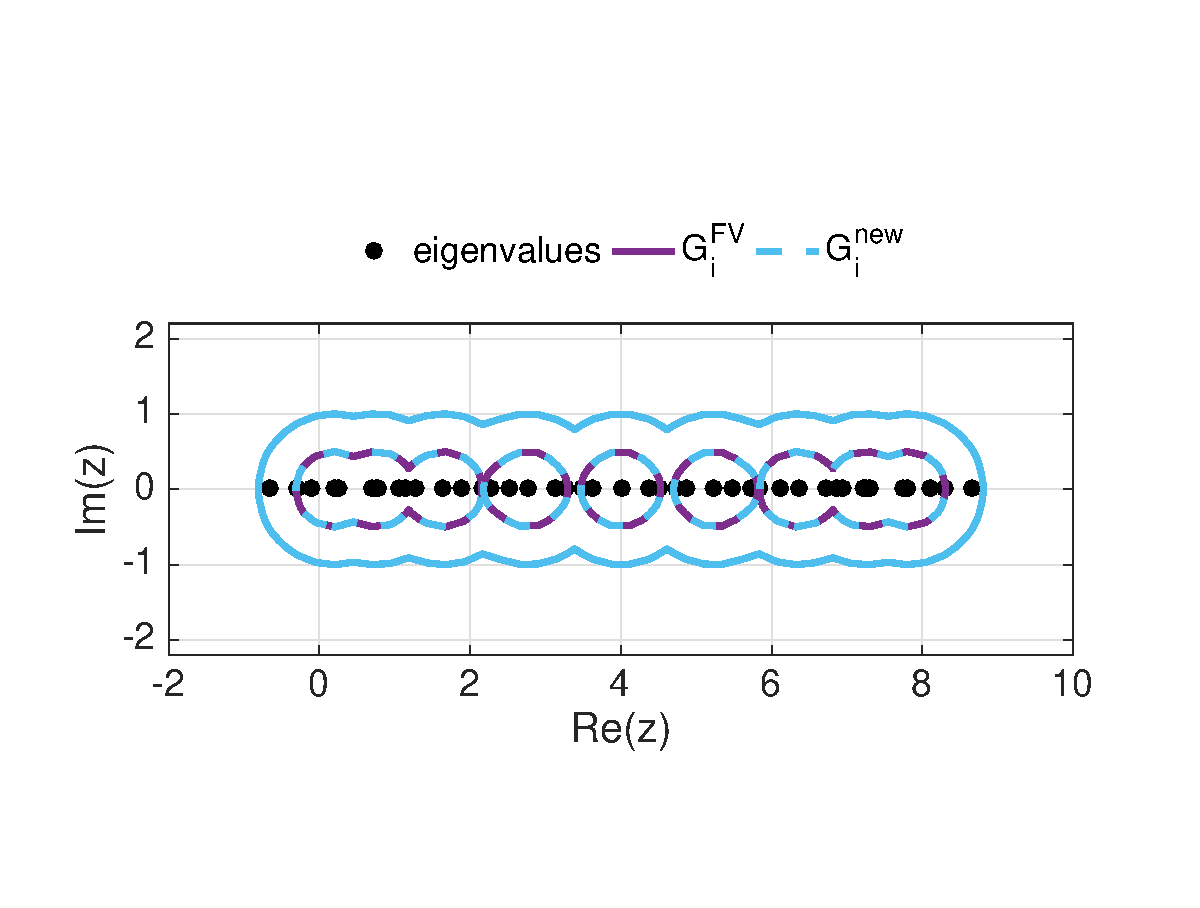
\includegraphics[width=0.49\linewidth]{figures/Example417_b1}
% 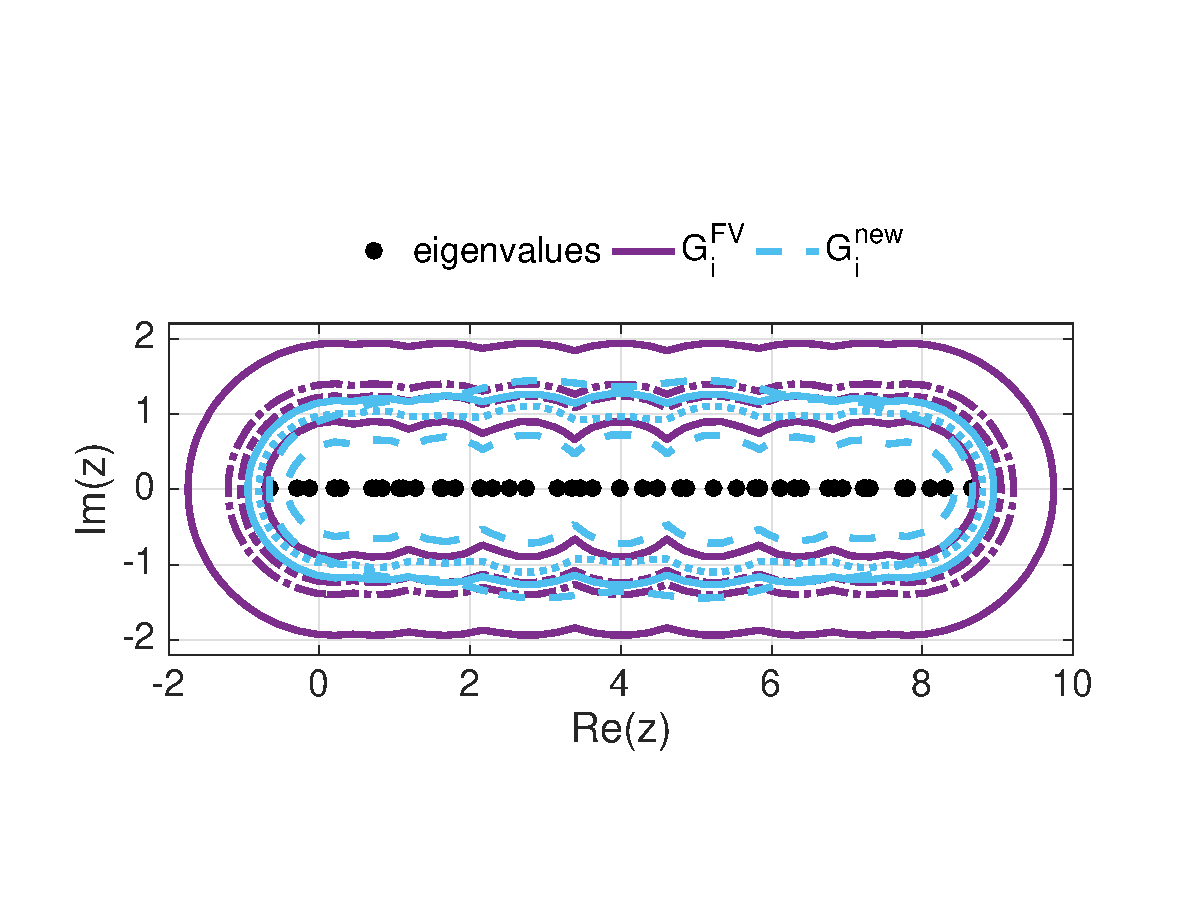
\includegraphics[width=0.49\linewidth]{figures/Example417_a1}
% \vspace{-1em}
% \caption{Eigenvalue inclusion regions obtained from the sets
% $G_i^{\text{new}}$ and $G_i^{\text{FV}}$ of Example~\ref{ex:BDiDo:inclusion2}.}
% \label{fig:BDiDo:ex:inclusion2}
% \end{figure}
% %
% \begin{figure}[h!]
% \centering
% 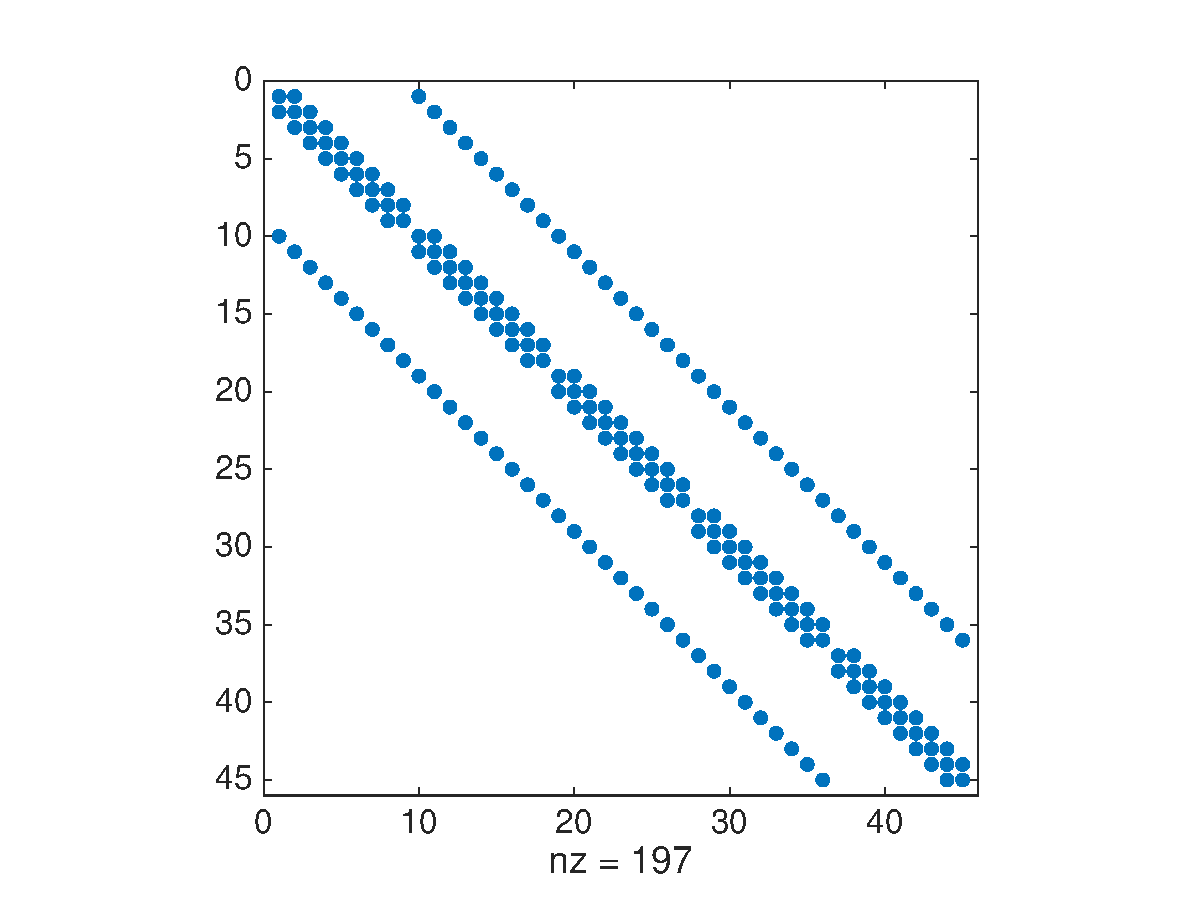
\includegraphics[width=0.4\linewidth]{figures/Example417_b2}
% 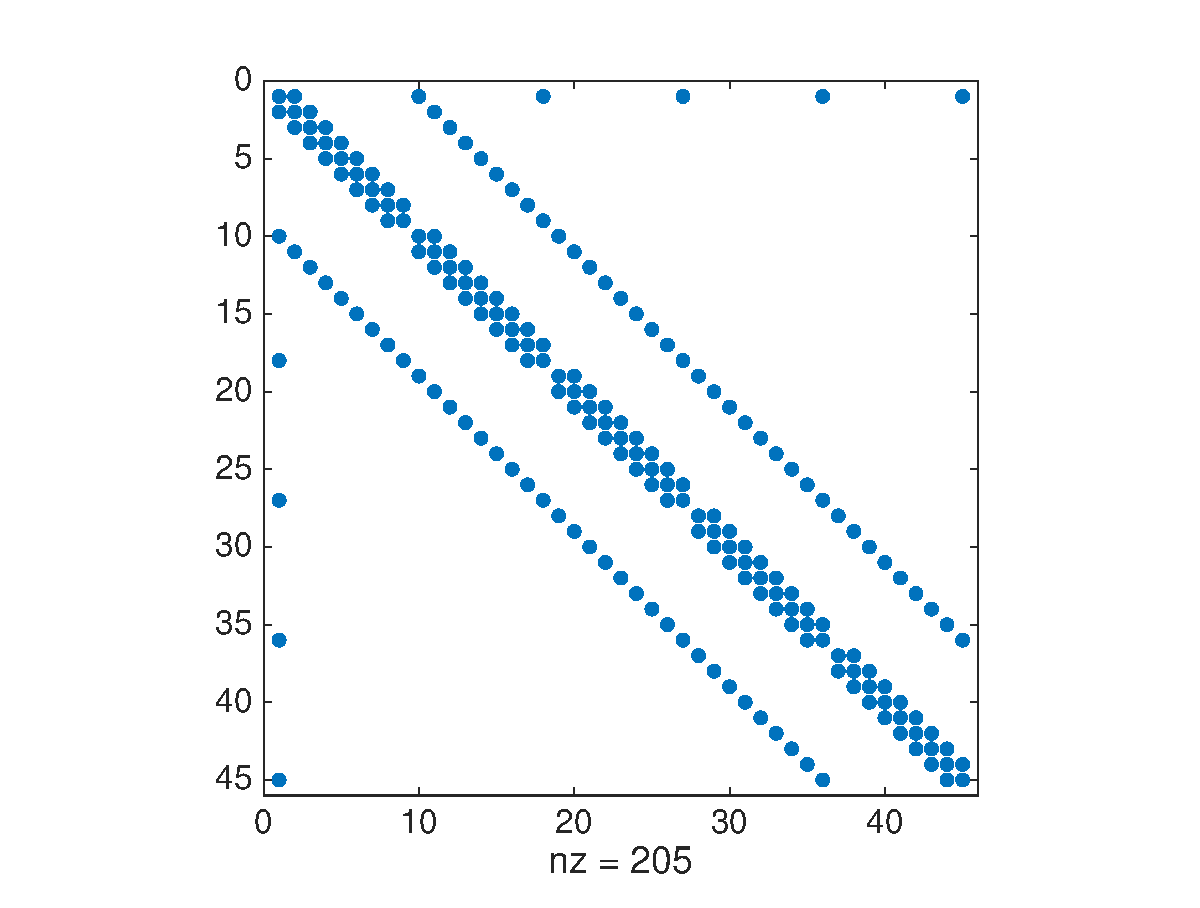
\includegraphics[width=0.4\linewidth]{figures/Example417_a2}
% \caption{Sparsity pattern of the matrices of Example~\ref{ex:BDiDo:inclusion2}.}
% \label{fig:BDiDo:ex:inclusion2_b}
% \end{figure}
% %
% }\end{example}

% \begin{example}\label{ex:BDiDo:inclusion3}{\textrm
% Consider the  nonsymmetric block tridiagonal matrix $\A$ as in Example~\ref{ex:BDiDo:symm}, i.e.,
% \[\A~=(\R\otimes \I)(\T\otimes \I+ \I\otimes~\T) \;\;\in\;\;\mathbb{R}^{81\times 81},\]
% where $\T=\textrm{tridiag}(-1,2,-1) \in {\mathbb R}^{9\times 9}$ and
% $\R\in\mathbb{R}^{9\times 9}$ is a random diagonal matrix with nonzero integer
% entries between $0$ and $10$ and constructed in \texttt{MATLAB} with the command
% \texttt{\R = diag(ceil(10*rand(9,1)))}. Thus, $\A$ is of the form
% \eqref{eq:BDiDo:blocktridiag} with random tridiagonal Toeplitz matrices
% $\A_i$, and random constant diagonal matrices $\B_i$ and $\C_i$ for all $i$ and
% has the eigenvalues\td{\textbf{add:}eigenvalues of this matrix.}
% (computed in \texttt{MATLAB} and rounded to five significant digits).
% %
% The boundaries of the corresponding sets $G_i^{\text{new}}$ and $G_i^{FV}$ for
% $i=1,\ldots,9$ are shown on Figure~\ref{fig:BDiDo:ex:inclusion3}.
% %
% \begin{figure}[h!]
% \centering
% \includegraphics[width=0.49\linewidth]{figures/Example416a}
% \includegraphics[width=0.49\linewidth]{figures/Example416b}
% \caption{Eigenvalue inclusion regions obtained from the sets
% $G_i^{\text{new}}$ and $G_i^{\text{FV}}$ of Example~\ref{ex:BDiDo:inclusion3} for two different ramdom matrices $\R$.}
% \label{fig:BDiDo:ex:inclusion2}
% \end{figure}
% %
% The sets $G_i^{\text{new}}$ give the same inclusion regions for the
% eigenvalues than the sets $G_i^{\text{FV}}$ since the off diagonal blocks are still diagonal, nevertheless both inclusion regions are tighter than the usual Gershgorin circles.
% }\end{example}
%
We now present an example of the inclusion sets for the eigenvalues of a  matrix
\begin{equation}\label{eq:BDiDo:ConvDiffMat}
\A=\left[
  \begin{array}{ccc}
             \matAHhat       & \e_{m}\otimes\matBH   &    0            \\
    \e_{m}^{\Tr}\otimes\matC  &   \matA      & \e_{1}^{\Tr}\otimes\matB \\
                   0         & \e_{1}\otimes\matCh &        \matAhhat  \\
  \end{array}
\right]\;\in\;{\mathbb R}^{N(2m+1)\times N(2m+1)},
\end{equation}
obtained, for example, from a Shishkin mesh discretization of the 2D convection-diffusion problems of type \eqref{eq:2D:2Dbvp} studied in Chapter~\ref{ch:2D}.

% \newpage
\begin{example}\label{ex:BDiDo:inclusionconvdiff1}{\textrm
Consider the  nonsymmetric block tridiagonal matrix
\begin{equation}\label{eq:BDiDo:ConvDiffMat1}
\A=\left[
  \begin{array}{ccc}
 \matA  & \matB  &      0     \\
     \matC  &   \matA &  \matB     \\
      0     & \matC  &  \matA  \\
  \end{array}
\right]\;\in\;{\mathbb R}^{15 \times 15},
\end{equation}
where $\matA=\mathrm{tridiag}(-36,108,-36)\in\mathbb{R}^{5\times5}$, $\matB=\mathrm{diag}(-16)\in\mathbb{R}^{5\times5}$ and
$\matC=\mathrm{diag}(-20)~\in~\mathbb{R}^{5\times5}$, i.e., we have a matrix of type \eqref{eq:BDiDo:ConvDiffMat} with $N=5$, $m=1$ and $\matAHhat=\matAhhat=\matA$, $\matBH=\matB$, and  $\matCh=\matC$. \textnormal{Figure~\ref{fig:BDiDo:ex:inclusion3}}
shows the $15$ eigenvalues computed in \textnormal{\texttt{MATLAB}} and rounded to five significant digits as well as the boundaries of the corresponding sets $G_i^{\text{new}}$, and $G_i^{\text{FV}}$ for $i=1,2,3$.
%
\begin{figure}[tbph]
\centering
\vspace*{-0.4cm}
\includegraphics[width=0.49\linewidth]{figures/Example416_b1}
\includegraphics[width=0.49\linewidth]{figures/Example416_b2}
% \vspace*{-0.5cm}
\caption{Eigenvalue inclusion regions obtained from the sets
$G_i^{\text{new}}$ and $G_i^{\text{FV}}$ for the matrix \eqref{eq:BDiDo:ConvDiffMat1} of Example~\ref{ex:BDiDo:inclusionconvdiff1}.}
\label{fig:BDiDo:ex:inclusion3}
\end{figure}

The figure shows that  sets $G_i^{\text{new}}$ give the same inclusion regions
for the eigenvalues than the sets $G_i^{\text{FV}}$ (both inclusion regions are tighter than the usual Gershgorin circles); this is to be expected since the off-diagonal blocks are multiples of the identity matrix and the sets $G_i^{\text{new}}$ reduce to the sets $G_i^{\text{FV}}$. However, by changing the structure of the
off-diagonal blocks (we make the upper right corner of each upper off-diagonal block and the lower left entry of each lower off-diagonal block equal to~$10$), the eigenvalues do not shift much, nevertheless, the sets are no longer equal and once again the new sets $G_i^{\text{new}}$ present much tighter inclusion regions than the sets $G_i^{\text{FV}}$ - see the right side of \textnormal{Figure~\ref{fig:BDiDo:ex:inclusion3}}
}\end{example}

\begin{example}\label{ex:BDiDo:inclusionconvdiff2}{\textrm
Consider the  nonsymmetric block tridiagonal matrix \eqref{eq:BDiDo:ConvDiffMat1} from \textnormal{Example~\ref{ex:BDiDo:inclusionconvdiff1}}
where $\matA=\mathrm{tridiag}(-36,108,-36)\in\mathbb{R}^{5\times5}$, but now we choose the off-diagonal blocks $\matB$ and $\matC$ as $5\times5$ diagonal matrices with random positive integer entries between $0$ and $9$ using the \textnormal{\texttt{MATLAB}} command \textnormal{\texttt{diag(floor(10*rand(5,1)))}}. \textnormal{Figure~\ref{fig:BDiDo:ex:inclusion4}} once again
shows the $15$ eigenvalues as well as the boundaries of the corresponding sets $G_i^{\text{new}}$, and $G_i^{\text{FV}}$ for $i=1,2,3$.
%
\begin{figure}[tbph]
\centering
\vspace*{-0.5cm}
\includegraphics[width=0.9\linewidth]{figures/Example417}
\vspace*{-0.7cm}
\caption{Eigenvalue inclusion regions obtained from the sets
$G_i^{\text{new}}$ and $G_i^{\text{FV}}$ for the matrix \eqref{eq:BDiDo:ConvDiffMat1} of Example~\ref{ex:BDiDo:inclusionconvdiff2}.}
\label{fig:BDiDo:ex:inclusion4}
\end{figure}

\textnormal{Figure~\ref{fig:BDiDo:ex:inclusion4}} once again shows that sets $G_i^{\text{new}}$ present much tighter incusion regions than the sets $G_i^{\text{FV}}$.
In the context of convection diffusion equations, a coefficient matrix with the structure given by this example might correspond to having variable coefficients in equation~\eqref{eq:2D:2Dbvp} instead of constant ones, like it is the case for the matrix in Example~\ref{ex:BDiDo:inclusionconvdiff1}.
}\end{example}



\begin{example}\label{ex:BDiDo:inclusionconvdiff3}{\textrm
Consider the  nonsymmetric block tridiagonal matrix arising from the Shishkin mesh discretization of the convection-diffusion model problem \eqref{eq:2D:2Dbvp} with $\epsilon=10^{-4}$, using $16$ intervals in the $x$-direction and $8$ intervals in the $y$-direction (see next chapter) yielding a matrix of type \eqref{eq:BDiDo:ConvDiffMat} with $N=15$ and $m=7$. \textnormal{Figure~\ref{fig:BDiDo:ex:inclusion5}} shows the eigenvalues of the matrix as well as the boundaries of the corresponding sets $G_i^{\text{new}}$, and $G_i^{\text{FV}}$ for $i=1,\ldots,105$.
%
\begin{figure}[tbph]
\centering
\vspace*{-0.5cm}
\includegraphics[width=0.6\linewidth]{figures/Example418}
\vspace*{-0.2cm}
\caption{Eigenvalue inclusion regions obtained from the sets
$G_i^{\text{new}}$ and $G_i^{\text{FV}}$ for the matrix \eqref{eq:BDiDo:ConvDiffMat1} of Example~\ref{ex:BDiDo:inclusionconvdiff3}.}
\label{fig:BDiDo:ex:inclusion5}
\end{figure}
%
Just like it is the case for \textnormal{Example~\ref{ex:BDiDo:inclusionconvdiff1}}, the sets $G_i^{\text{new}}$ present the same inclusion regions than the sets $G_i^{\text{FV}}$. As we have discussed before, this is due to the constant-coefficient nature of the problem. Even though the eigenvalues appear clustered together in 4 tight clusters, the difference in magnitude between the eigenvalues, caused by the convection-domitated characteristic of the problem, makes the inclusion regions cover a much larger part of the complex plane than expected (notice the scale in \textnormal{Figure~\ref{fig:BDiDo:ex:inclusion5}}). Moreover, the regions grow as the problem becomes more convection dominated, making the inclusion sets not very informative in the case of real world problems. It is important to note, however, that a different subdivision of the blocks of \eqref{eq:BDiDo:ConvDiffMat} might lead to tighter inclusion regions for these type of problems, a task that remains to be explored.
}\end{example}

% All experiments were computed on a 13-inch \texttt{Apple MacBook} computer model Mid 2010 with a 2,4 GHz Intel Core 2 Duo processor equipped with \texttt{MATLAB} version R2015b.
To complete this chapter, we present the definition of \emph{column} block diagonal dominance of matrices in the following Appendix.

\begin{subappendices}
\section{Column Block Diagonal Dominance of Matrices}
\label{App:BDiDo:ColBDiDo}
According to Definition~\ref{def:BDiDo:bdd} in Section~\ref{BDiDo:bounds}, the
property of \emph{column} block diagonal dominance of matrices is defined as
follows:
\begin{definition}\label{def:App:colbdd}
Consider a matrix of the form
%
\begin{equation}\label{eq:app:blockmatrix}
\A=[\A_{ij}]\quad
\mbox{with blocks $\A_{ij}\in\mathbb{C}^{m\times m}$ for $i,j=1,\dots,n$.}
\end{equation}
%
The matrix $\A$ is called \emph{column block diagonally dominant} (with respect
to the matrix norm $\|\cdot\|$) when the diagonal blocks $\A_{jj}$ are
nonsingular, and
%
\begin{equation}\label{eq:app:blocdiagdom1}
\sum_{\atopfrac{i=1}{i\neq j}}^{n} \|\A_{ij}\A_{jj}^{-1}\| \leq 1,
\quad \text{for $j=1,\dots,n$}.
\end{equation}
%
If strict inequality holds in \eqref{eq:app:blocdiagdom1} then $\A$ is called
\emph{column block strictly diagonally dominant} (with respect to the matrix
norm $\|\cdot\|$).
\end{definition}

Now, restricting our attention to block tridiagonal matrices of the form
\eqref{eq:BDiDo:blocktridiag} and following the notation of that chapter, in
order to obtain analogous bounds for the norms of the inverses of a column
block diagonally dominant matrix we fist need to set $\B_0~=~\C_n~=~0$, and
define the \emph{new} quantities
%
\begin{eqnarray*}
\tilde{\tau}_i   &\equiv& \frac{\|\C_i\A_i^{-1}\|}{1-\|\B_{i-1}\A_i^{-1}\|},
\quad \text{for $i=1,\ldots,n$}, \\
\tilde{\mu}_i &\equiv& \frac{\|\B_{i-1}\A_i^{-1}\|}{1-\|\C_{i}\A_i^{-1}\|},
\quad \text{for $i=1,\ldots,n$}.
\end{eqnarray*}
%
The column block diagonal dominance of $\A$ then implies that
$0~\leq ~\tilde{\tau}_i\leq~1$ and $0~\leq~\tilde{\mu}_i~\leq~1$.
Using these quantities we obtain the following result.
%
\begin{thm}
Let $A$  be as in \eqref{eq:BDiDo:blocktridiag} and suppose that
$\A_i^{-1}$ as well as $\B_i^{-1}$ and $\C_i^{-1}$ for $i=1,\ldots,n-1$ exist.
Suppose in addition that $\A$ is column block diagonally dominant, and that
%
\begin{equation}\label{eq:app:blktridom_b}
\|\C_1\A_1^{-1}\|<1 \quad \mbox{and} \quad \|\B_{n-1}\A_n^{-1}\|<1.
\end{equation}
%
Then $\A^{-1}=[\Z_{ij}]$ with
%
\begin{align}
\|\Z_{ij}\| & \leq  \|\Z_{ii}\| \prod_{k=i+1}^{j}\tilde{\mu}_k,
\quad\text{for all $i<j$}, \label{eq:app:offdiagbound1}\\
\|\Z_{ij}\| & \leq  \|\Z_{ii}\|\;\,\prod_{k=j}^{i-1}\tilde{\tau}_k,
\qquad\text{for all $i>j$},\label{eq:app:offdiagbound2}
\end{align}
%
with $\mu_k$ and $\tau_k$ given by \eqref{eq:BDiDo:mu} and \eqref{eq:BDiDo:tau}. Moreover, for $i=1,\dots,n$,
%
\begin{equation}\label{eq:app:diagbounds}
\frac{\|\I\|}
{\|\A_i\|+\tilde{\tau}_{i-1}\|\B_{i-1}\|+\tilde{\mu}_{i+1}\|\C_{i}\|}
\leq
\|\Z_{ii}\|
\leq
\frac{\|\I\|}
{\|\A_i^{-1}\|^{-1}-\tilde{\tau}_{i-1}\|\B_{i-1}\|-\tilde{\mu}_{i+1}\|\C_i\|},
\end{equation}
%
provided that the denominator of the upper bound is larger than zero,
and where we set $\B_0=\C_n=0$, and $\tilde{\tau}_0=\tilde{\mu}_{n+1}=0$.
\end{thm}

\begin{proof}
The proof of this theorem is completely analogous to the one of
Theorem~\ref{thm:BDiDo:blockbounds} for row block diagonally dominant matrices
when the necessary adaptations are made, i.e., by performing the following
changes:
%
\begin{itemize}

\item Formulate Lemma~\ref{lem:BDiDo:sequences} for the matrices $\X_i$ and
$\V_i$, showing that the sequence $\{\|\X_i\|\}_{i=1}^n$ is strictly increasing
while the sequence $\{\|\V_i\|\}_{i=1}^n$ is strictly decreasing.

\item Formulate Lemma~\ref{lem:BDiDo:nonsing} for the matrices
$\tilde{\L}_1=\tilde{\T}_1=\C_1\A_1^{-1}$, $\tilde{\T}_2=\I-\tilde{\T}_1\B_1\A_2^{-1}$,
$\tilde{\L}_i = \C_{i}\A_i^{-1}\tilde{\T}_i^{-1}$, and
$\tilde{\T}_i = \I-\tilde{\L}_{i-1}\B_{i-1}\A_i^{-1}$. Analogously for $\tilde{\M}_i$
and $\tilde{\W_i}$, etc.

\item Formulate Lemma~\ref{lem:BDiDo:recurrenceUY} for the matrices $\X_i$ and
$\V_i$, in particular showing that
$$
\X_i=-\X_{i+1}\tilde{\L}_i,\quad\mbox{and}\quad \V_i=-\V_{i-1}\tilde{\M}_i.
$$

\item In the proof of Theorem~\ref{thm:BDiDo:blockbounds} use the the
aforementioned results and use equation $\Z\A=\I$ instead of $\A\Z=\I$.
\end{itemize}
%
Following these changes and proceeding analogously to the proof
of Theorem~\ref{thm:BDiDo:blockbounds} yields the desired result.
\end{proof}

\end{subappendices}
\fi
